\chapter{\abbr{TOF} and \abbr{EC} Paddle Inefficiency Study Plots}\label{sec:app.tof_plots}

Shown below is are plots for the \abbr{TOF} and \abbr{EC} inefficiency studies. For completeness, all sectors are shown.

\section{\abbr{TOF} Inefficiency Study}
Sec.~\ref{sec:analysis.tof_fid} refers to this section for a complete view of the \abbr{TOF} study performed. All inefficiencies and cuts shown are for he $\pi^+$ and proton data. These inefficiencies and cuts are valid for the $\pi^-$ and all other negative charged tracks.
\begin{figure}[!ht]
  \centering
  \subfloat[][]{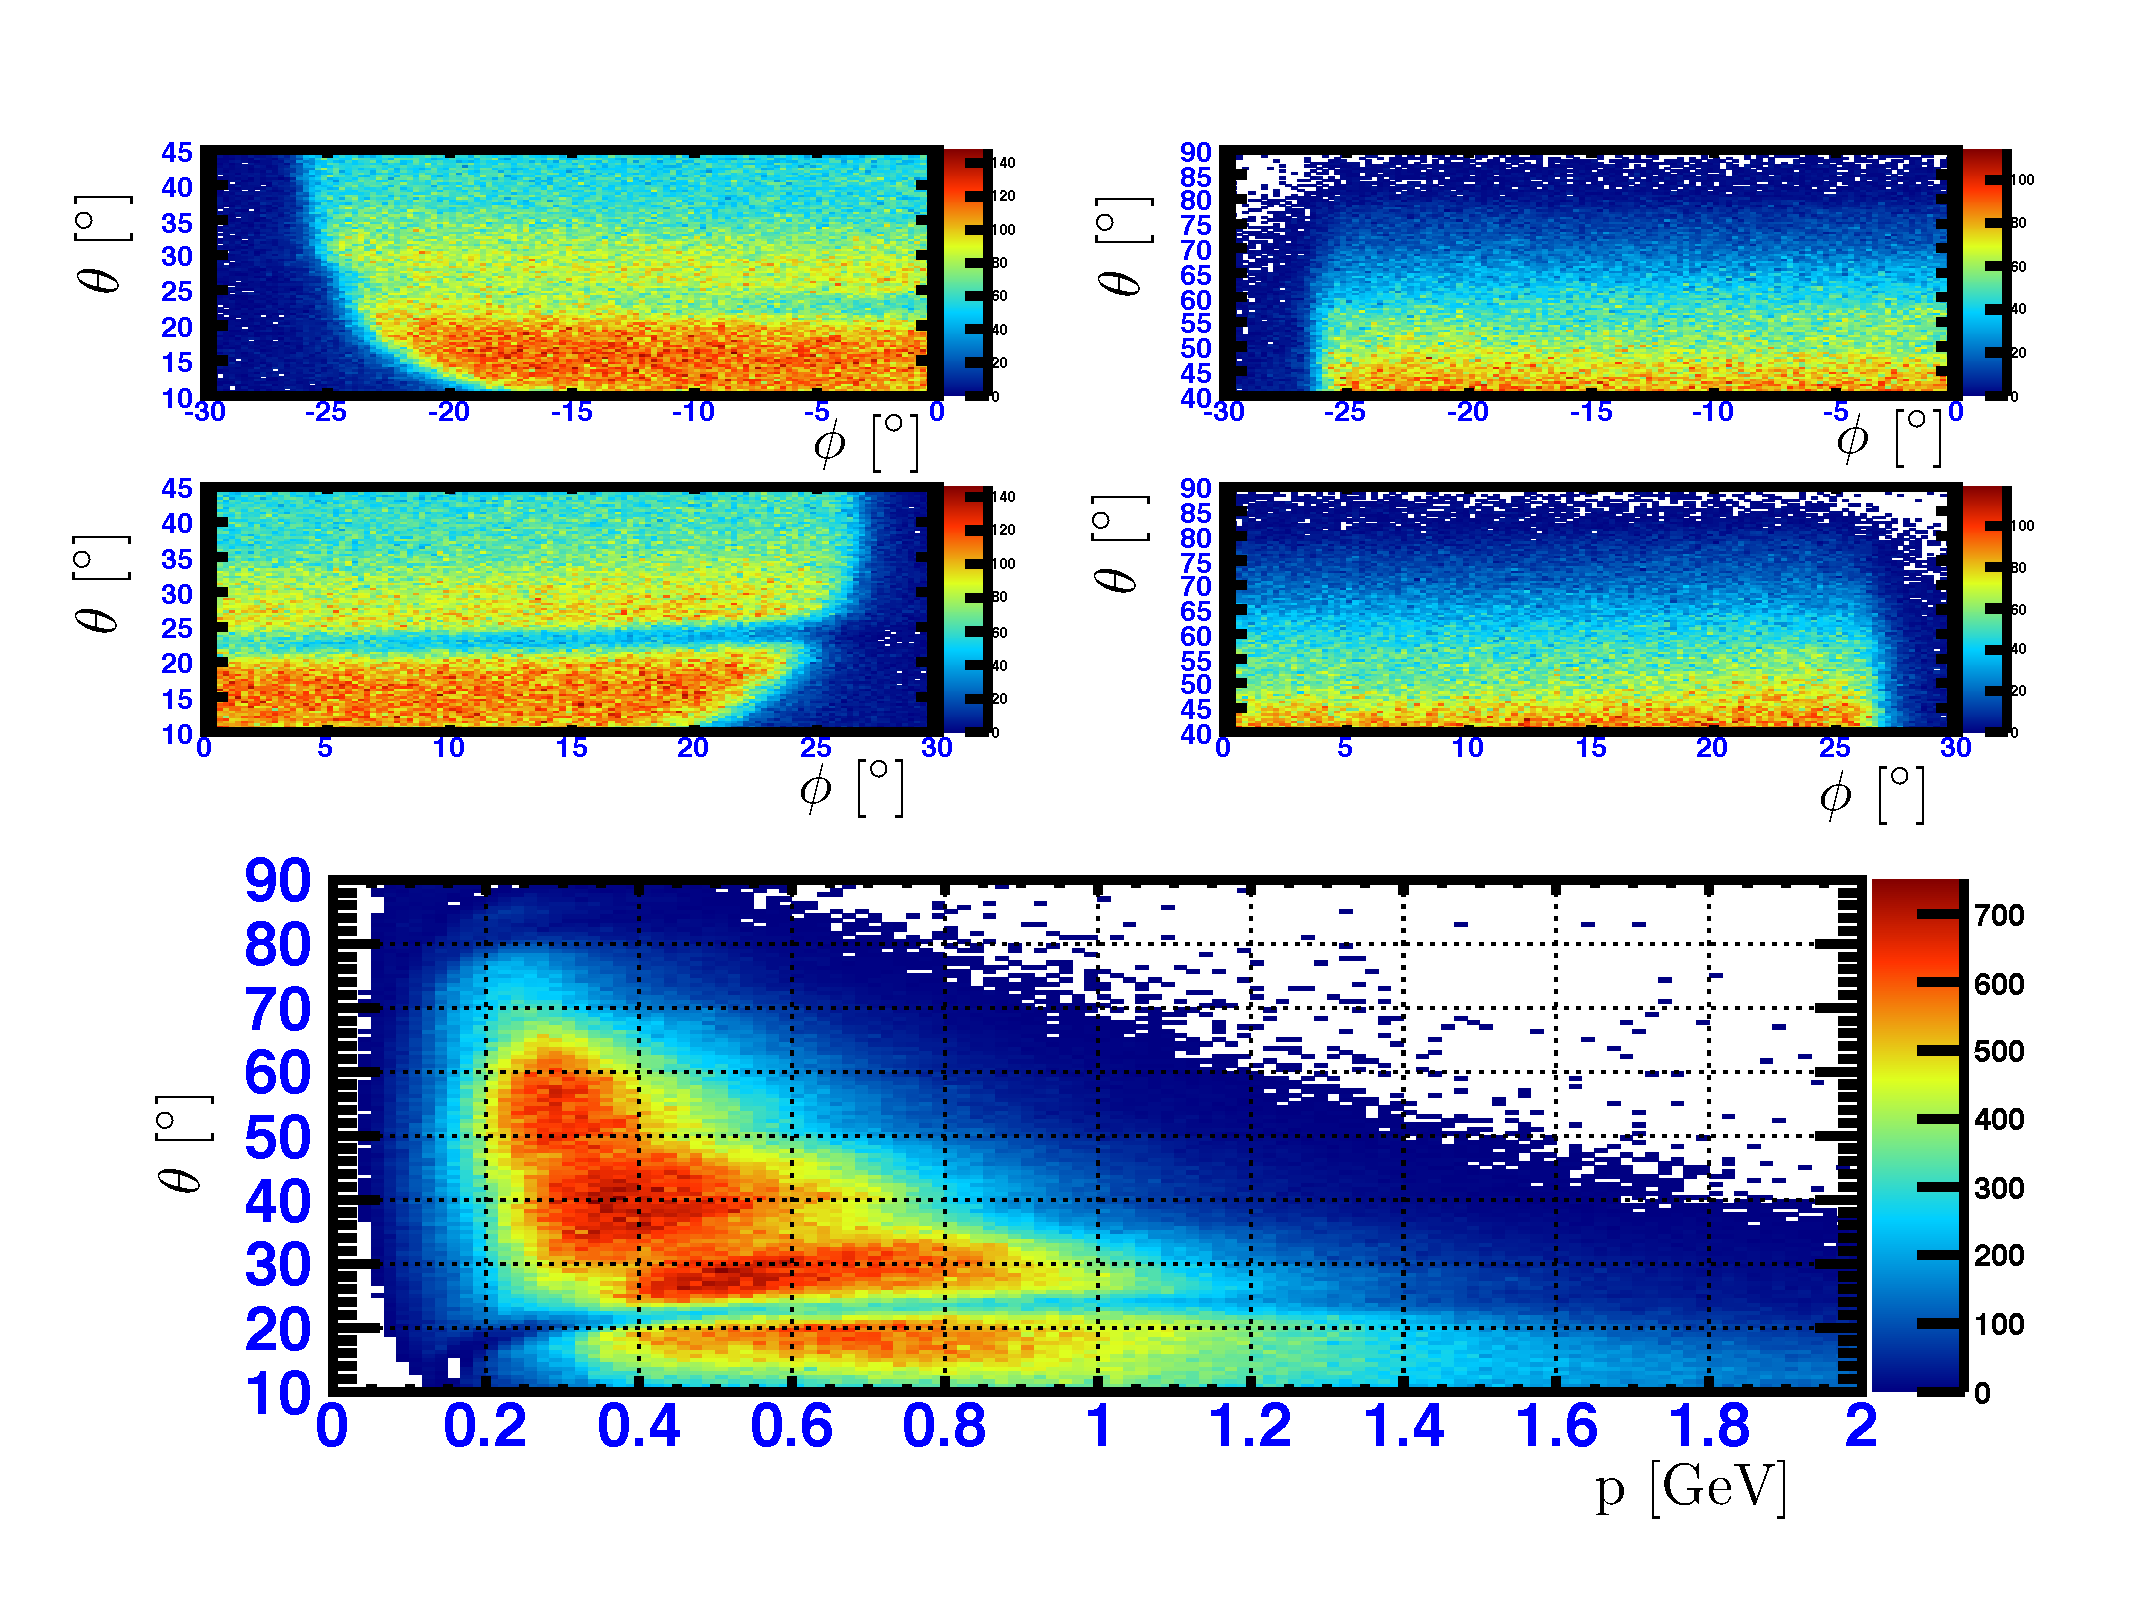
\includegraphics[width=\figwidth, height=3.5in,valign=c]{\grpath/analysis/FIDUCIAL_CUTS/TOF/RAW/pip_sec1.pdf}\label{fig:I}} \quad
  \\
  \subfloat[][]{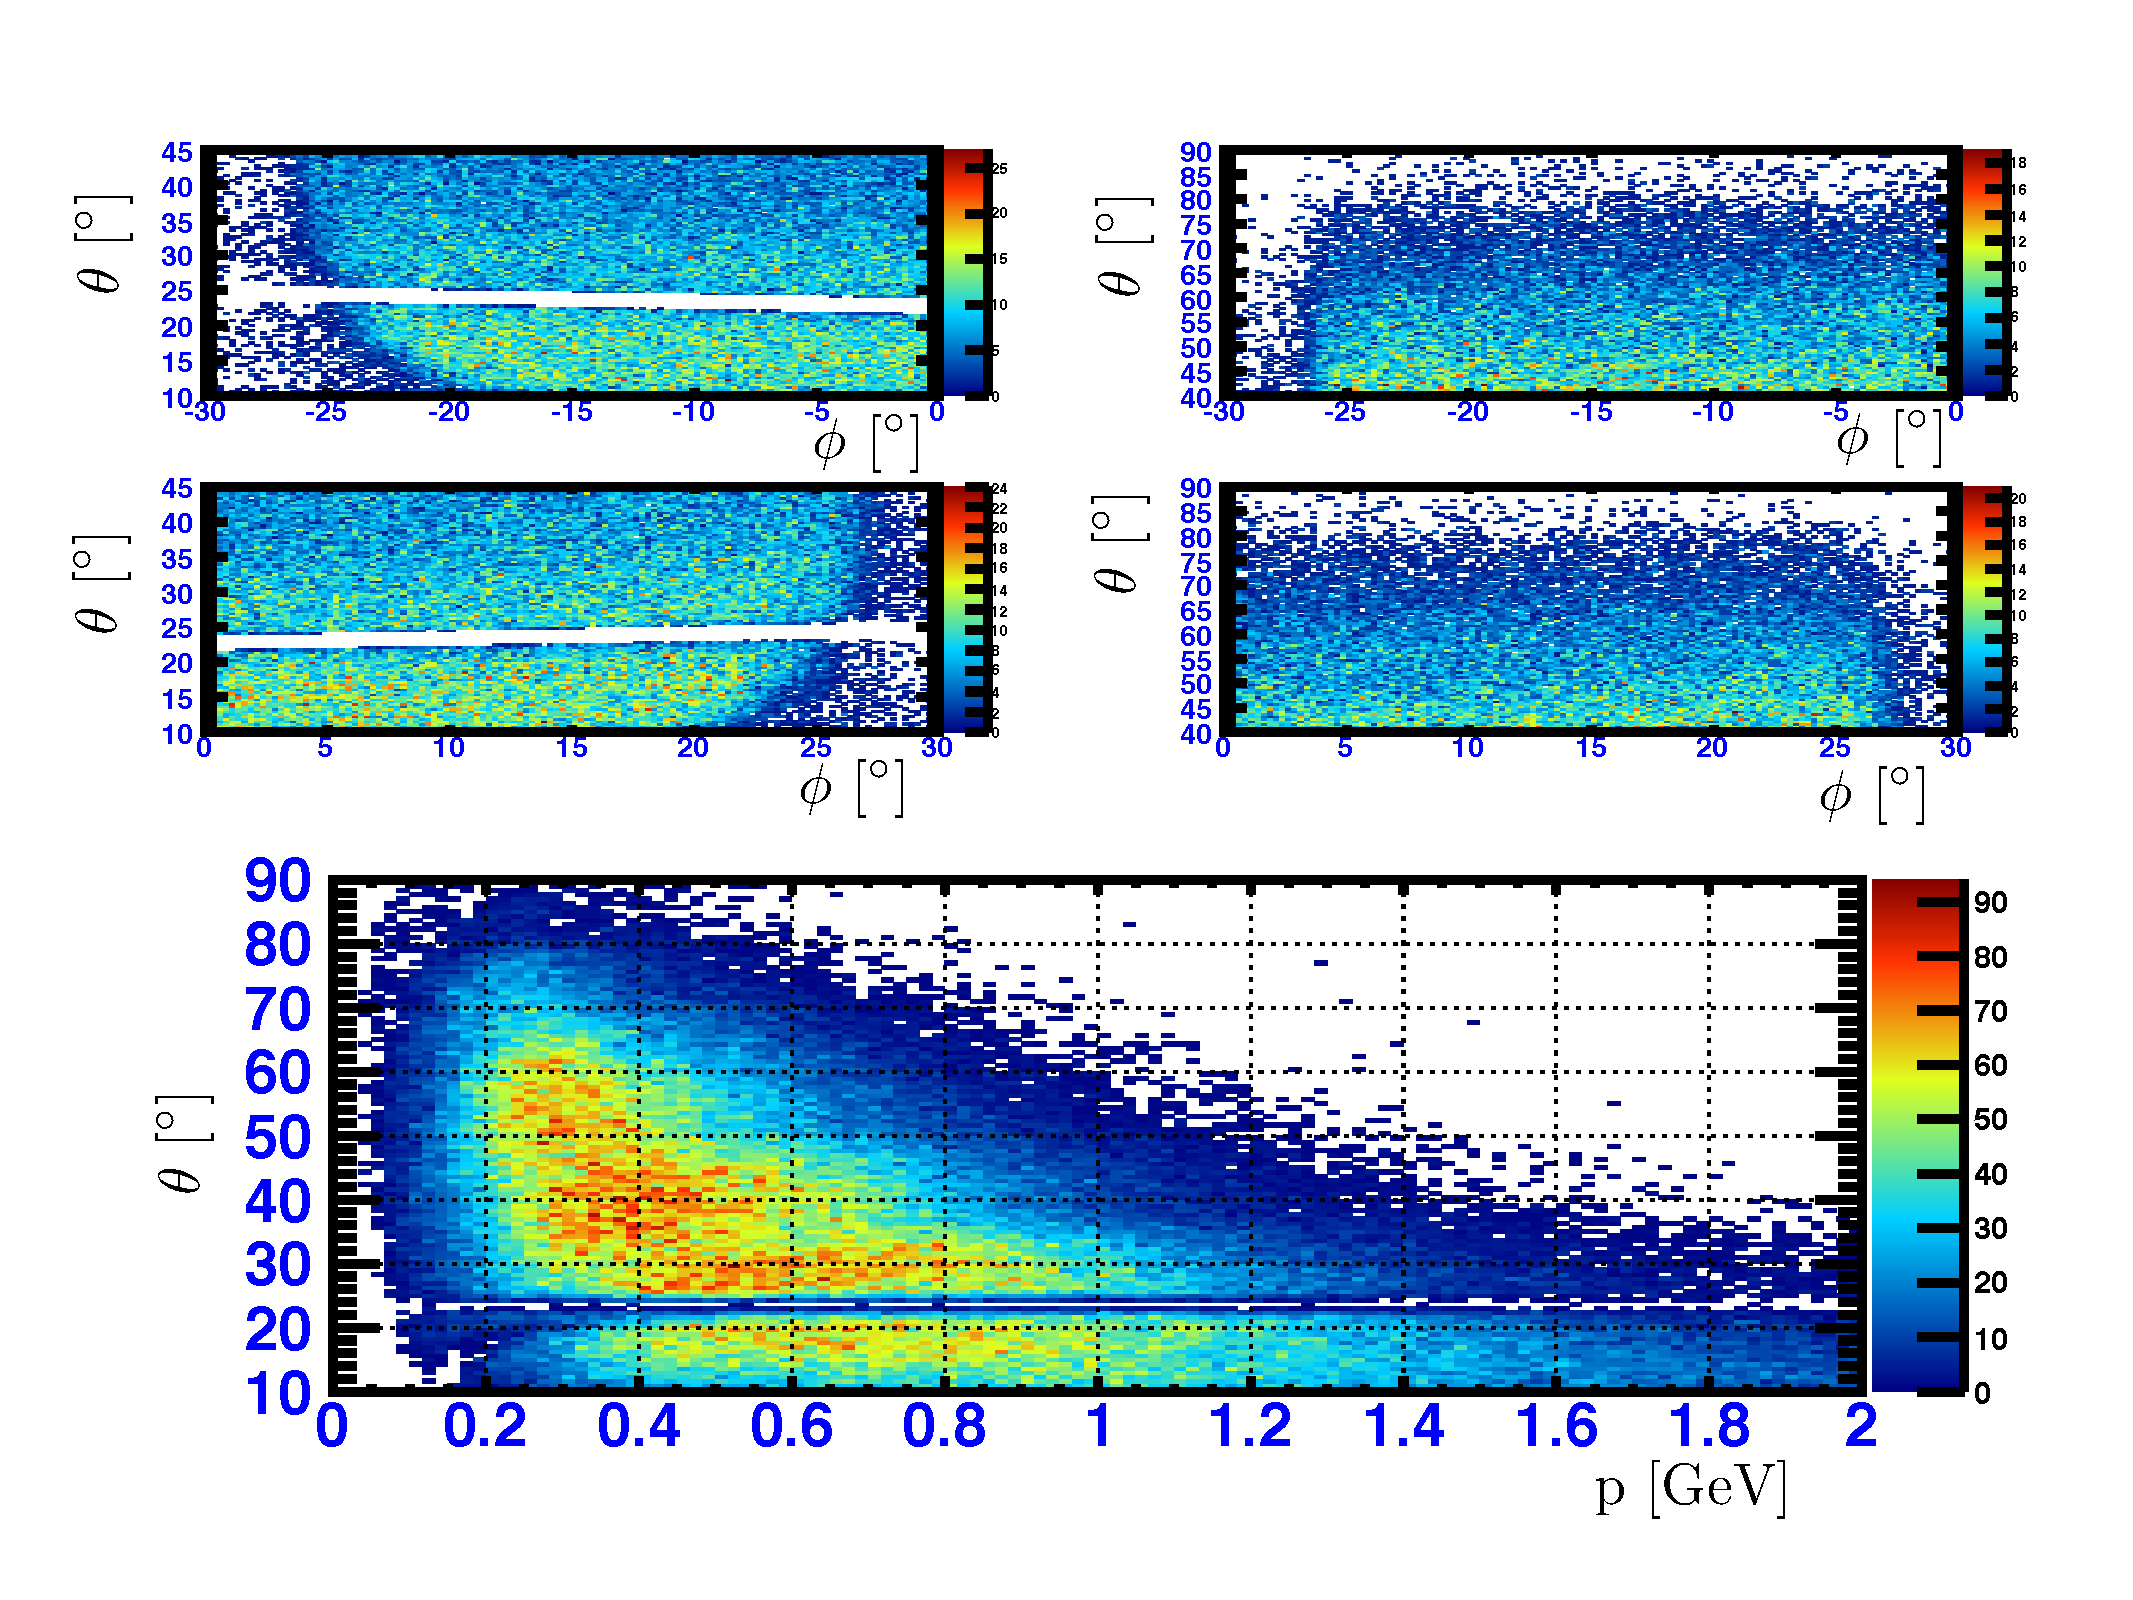
\includegraphics[width=\figwidth, height=3.5in,valign=c]{\grpath/analysis/FIDUCIAL_CUTS/TOF/KNOCK_OUT/pip_sec1_Knockout.pdf}\label{fig:II}} \\

      \caption {\abbr{TOF} inefficiency Plot for sector 1~(\ref{fig:I}). Inefficiency cut for $\pi^{+} \ $ and proton data ~(\ref{fig:II}). Notation same as in Fig.~\ref{fig:pos:tofcut_off}.}
        \label{fig:allI}
\end{figure}

\begin{figure}[!ht]
  \centering
  \subfloat[][]{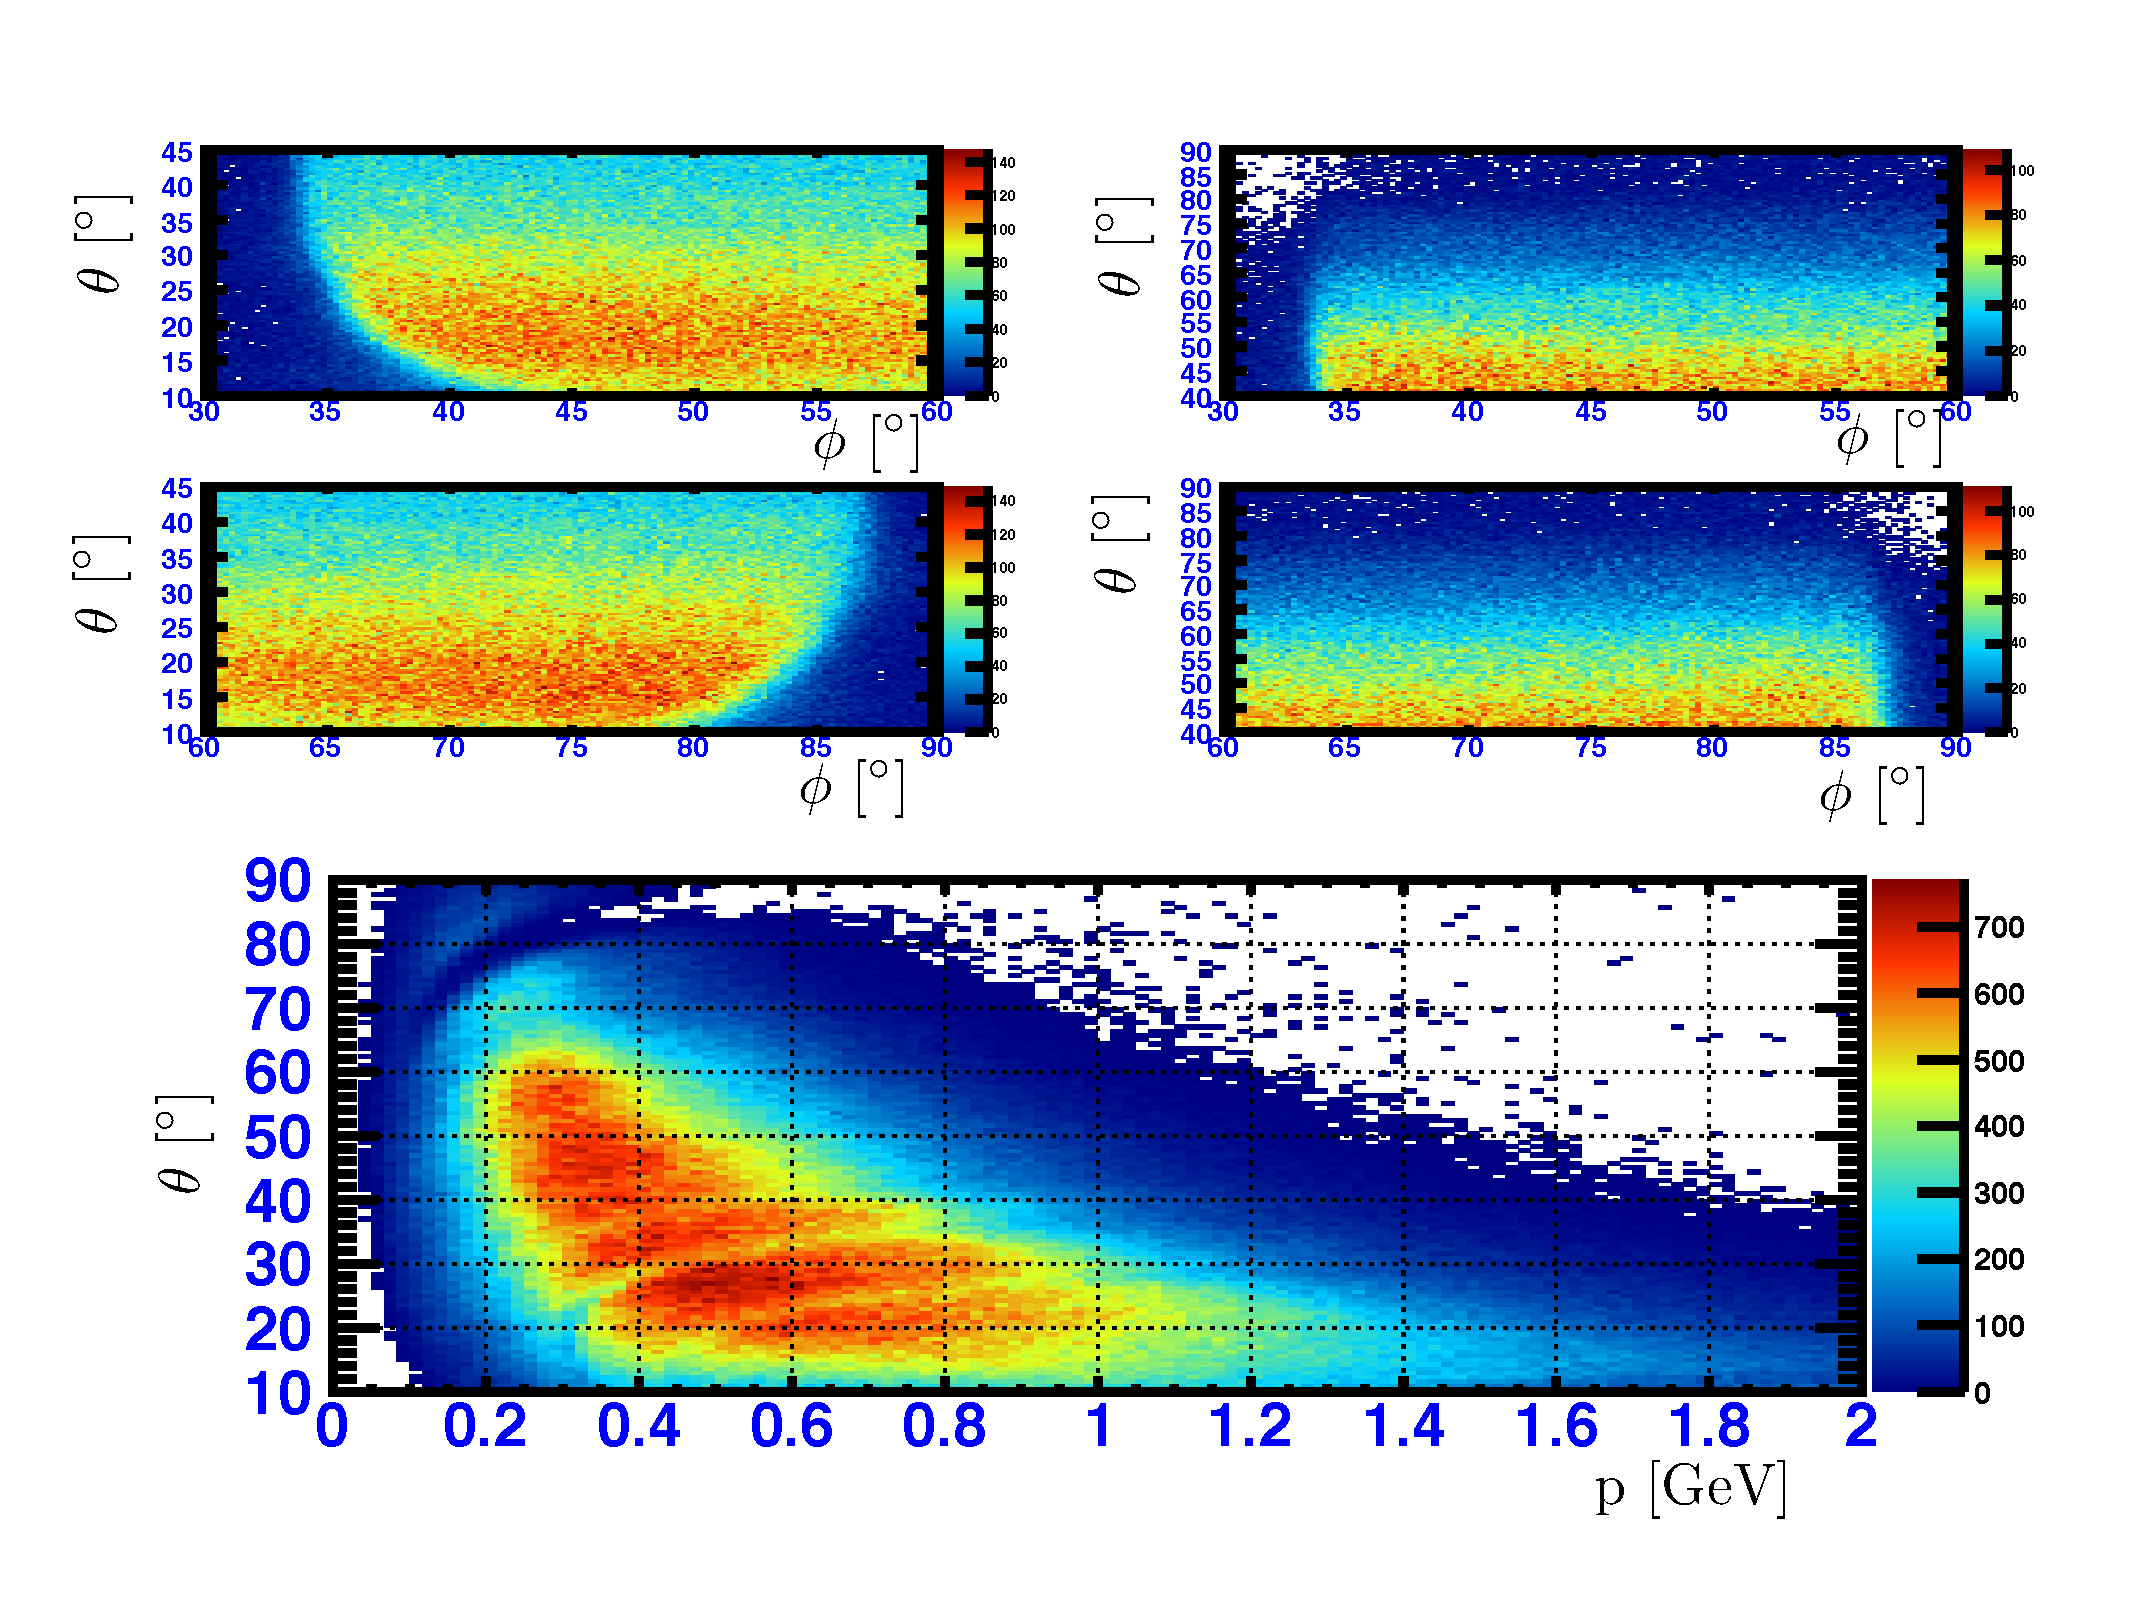
\includegraphics[width=\figwidth, height=3.5in,valign=c]{\grpath/analysis/FIDUCIAL_CUTS/TOF/RAW/pip_sec2.pdf}\label{fig:I_I}} \quad
  \\
  \subfloat[][]{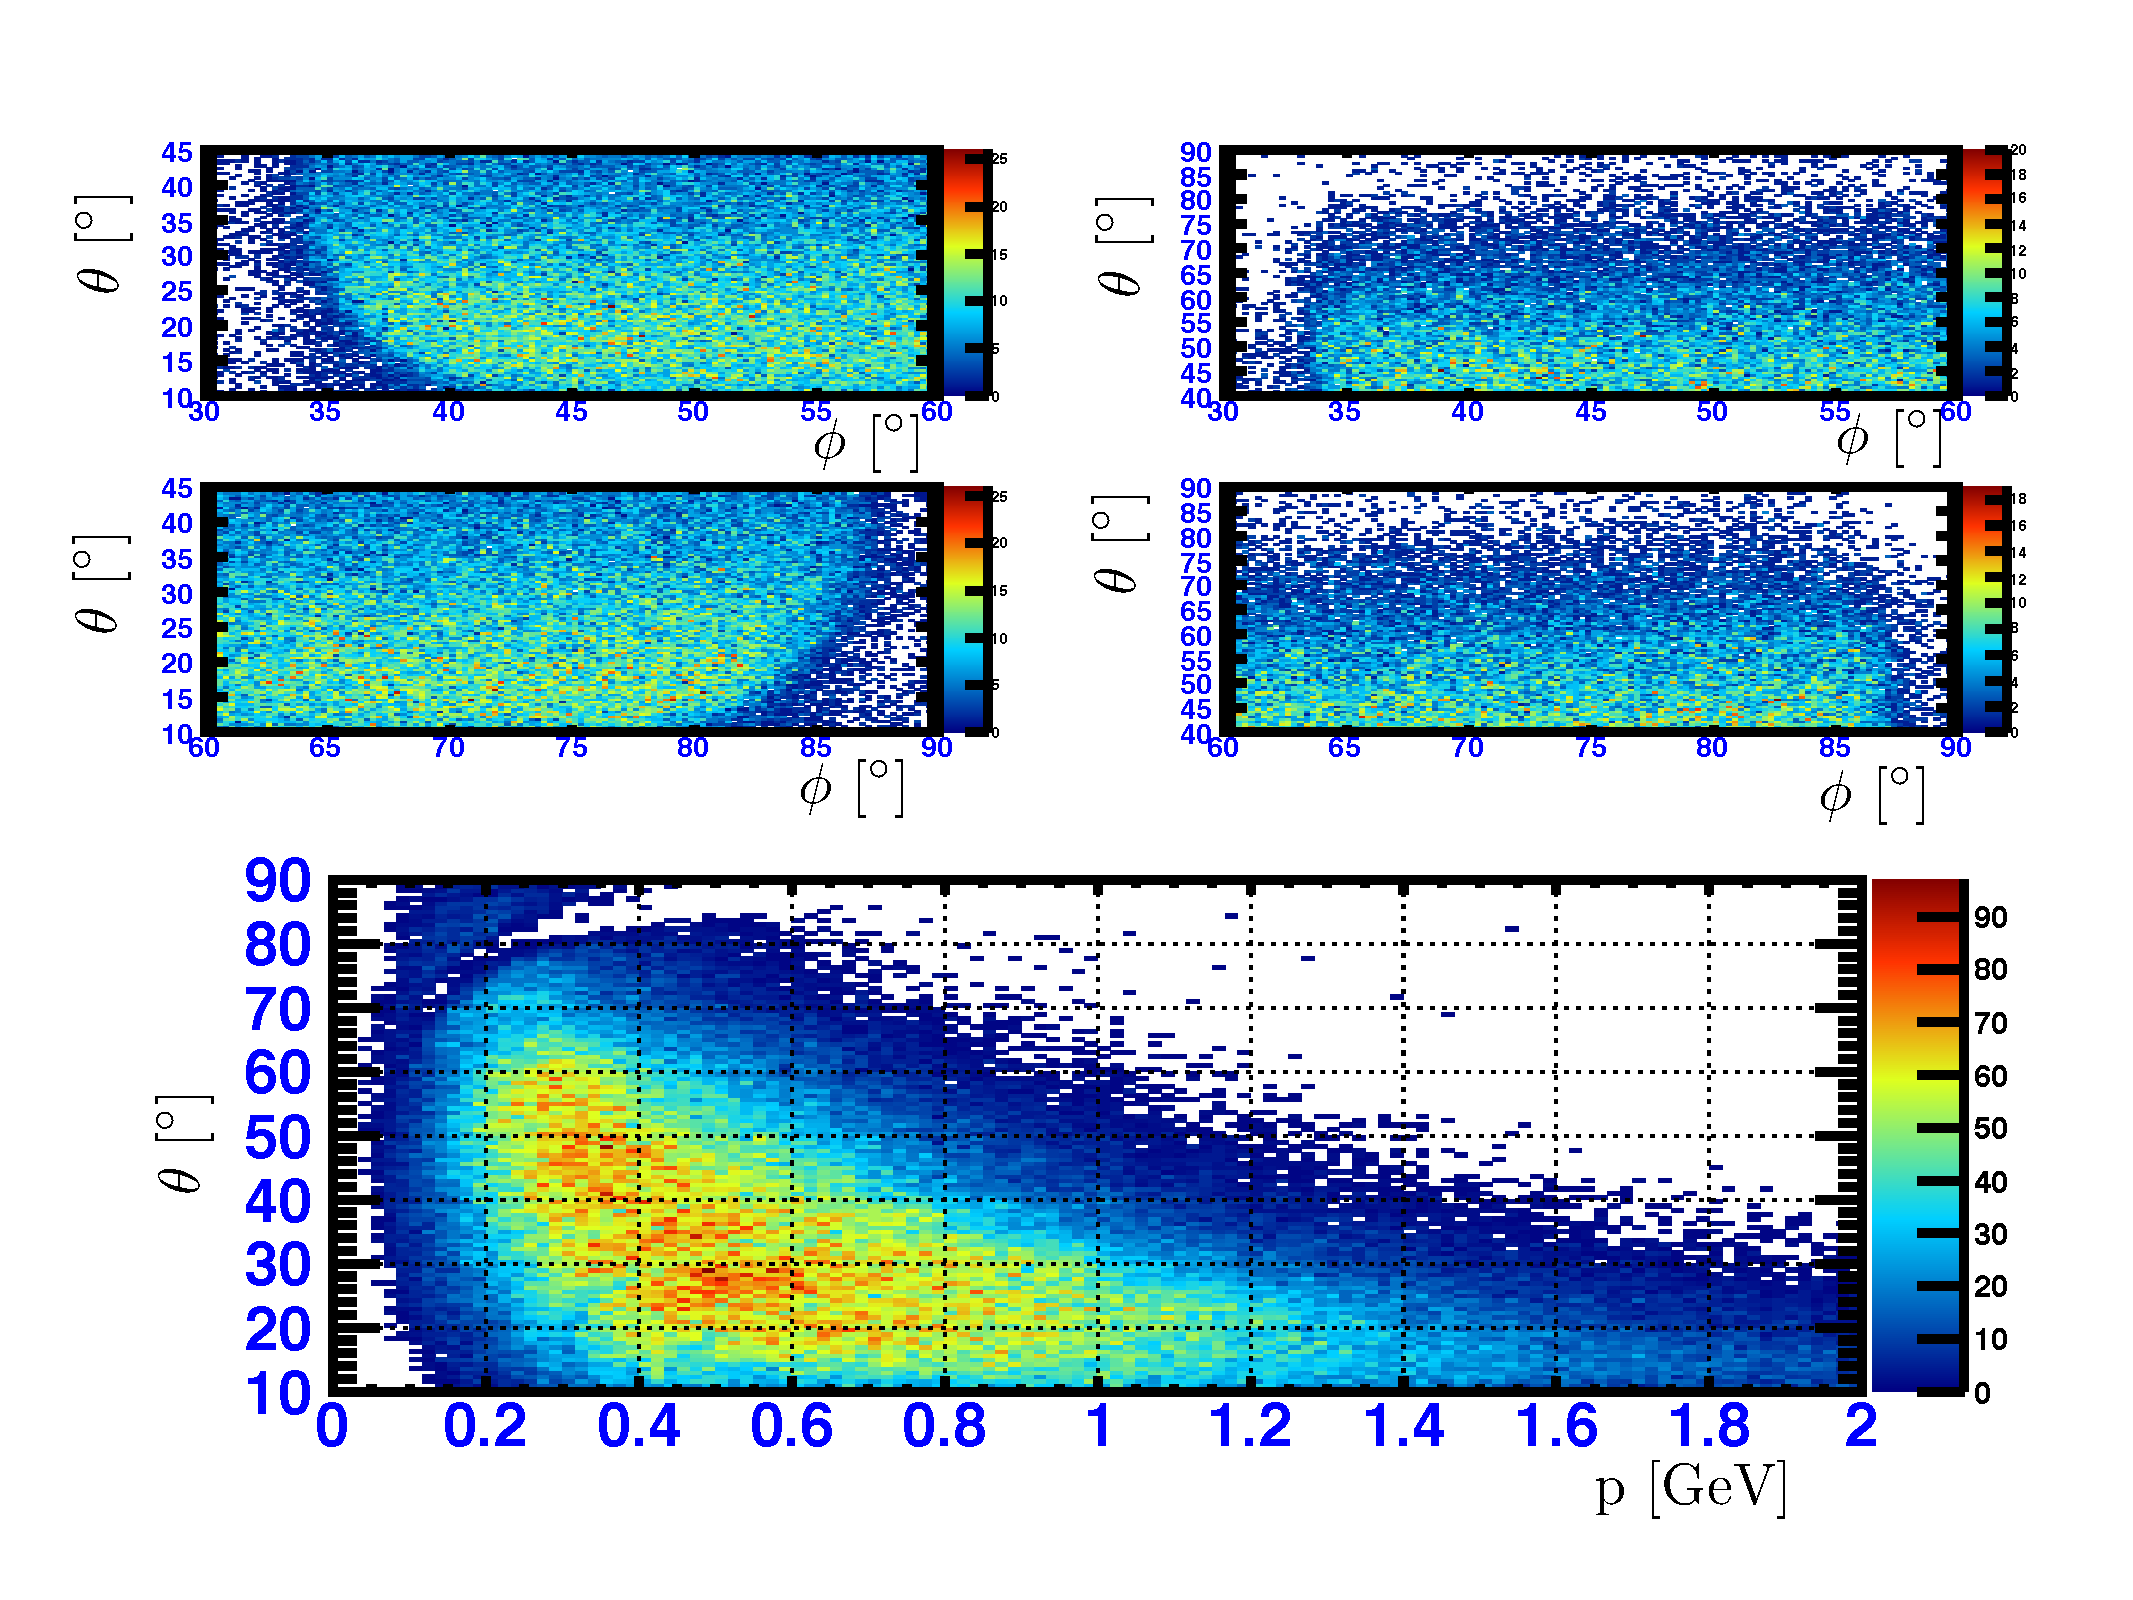
\includegraphics[width=\figwidth, height=3.5in,valign=c]{\grpath/analysis/FIDUCIAL_CUTS/TOF/KNOCK_OUT/pip_sec2_Knockout.pdf}\label{fig:II_I}} \\

      \caption {\abbr{TOF} inefficiency Plot for sector 2~(\ref{fig:I_I}). Inefficiency cut for $\pi^{+} \ $ and proton data ~(\ref{fig:II_I}). Notation same as in Fig.~\ref{fig:pos:tofcut_off}.}
        \label{fig:allI_I}
\end{figure}

\begin{figure}[!ht]
  \centering
  \subfloat[][]{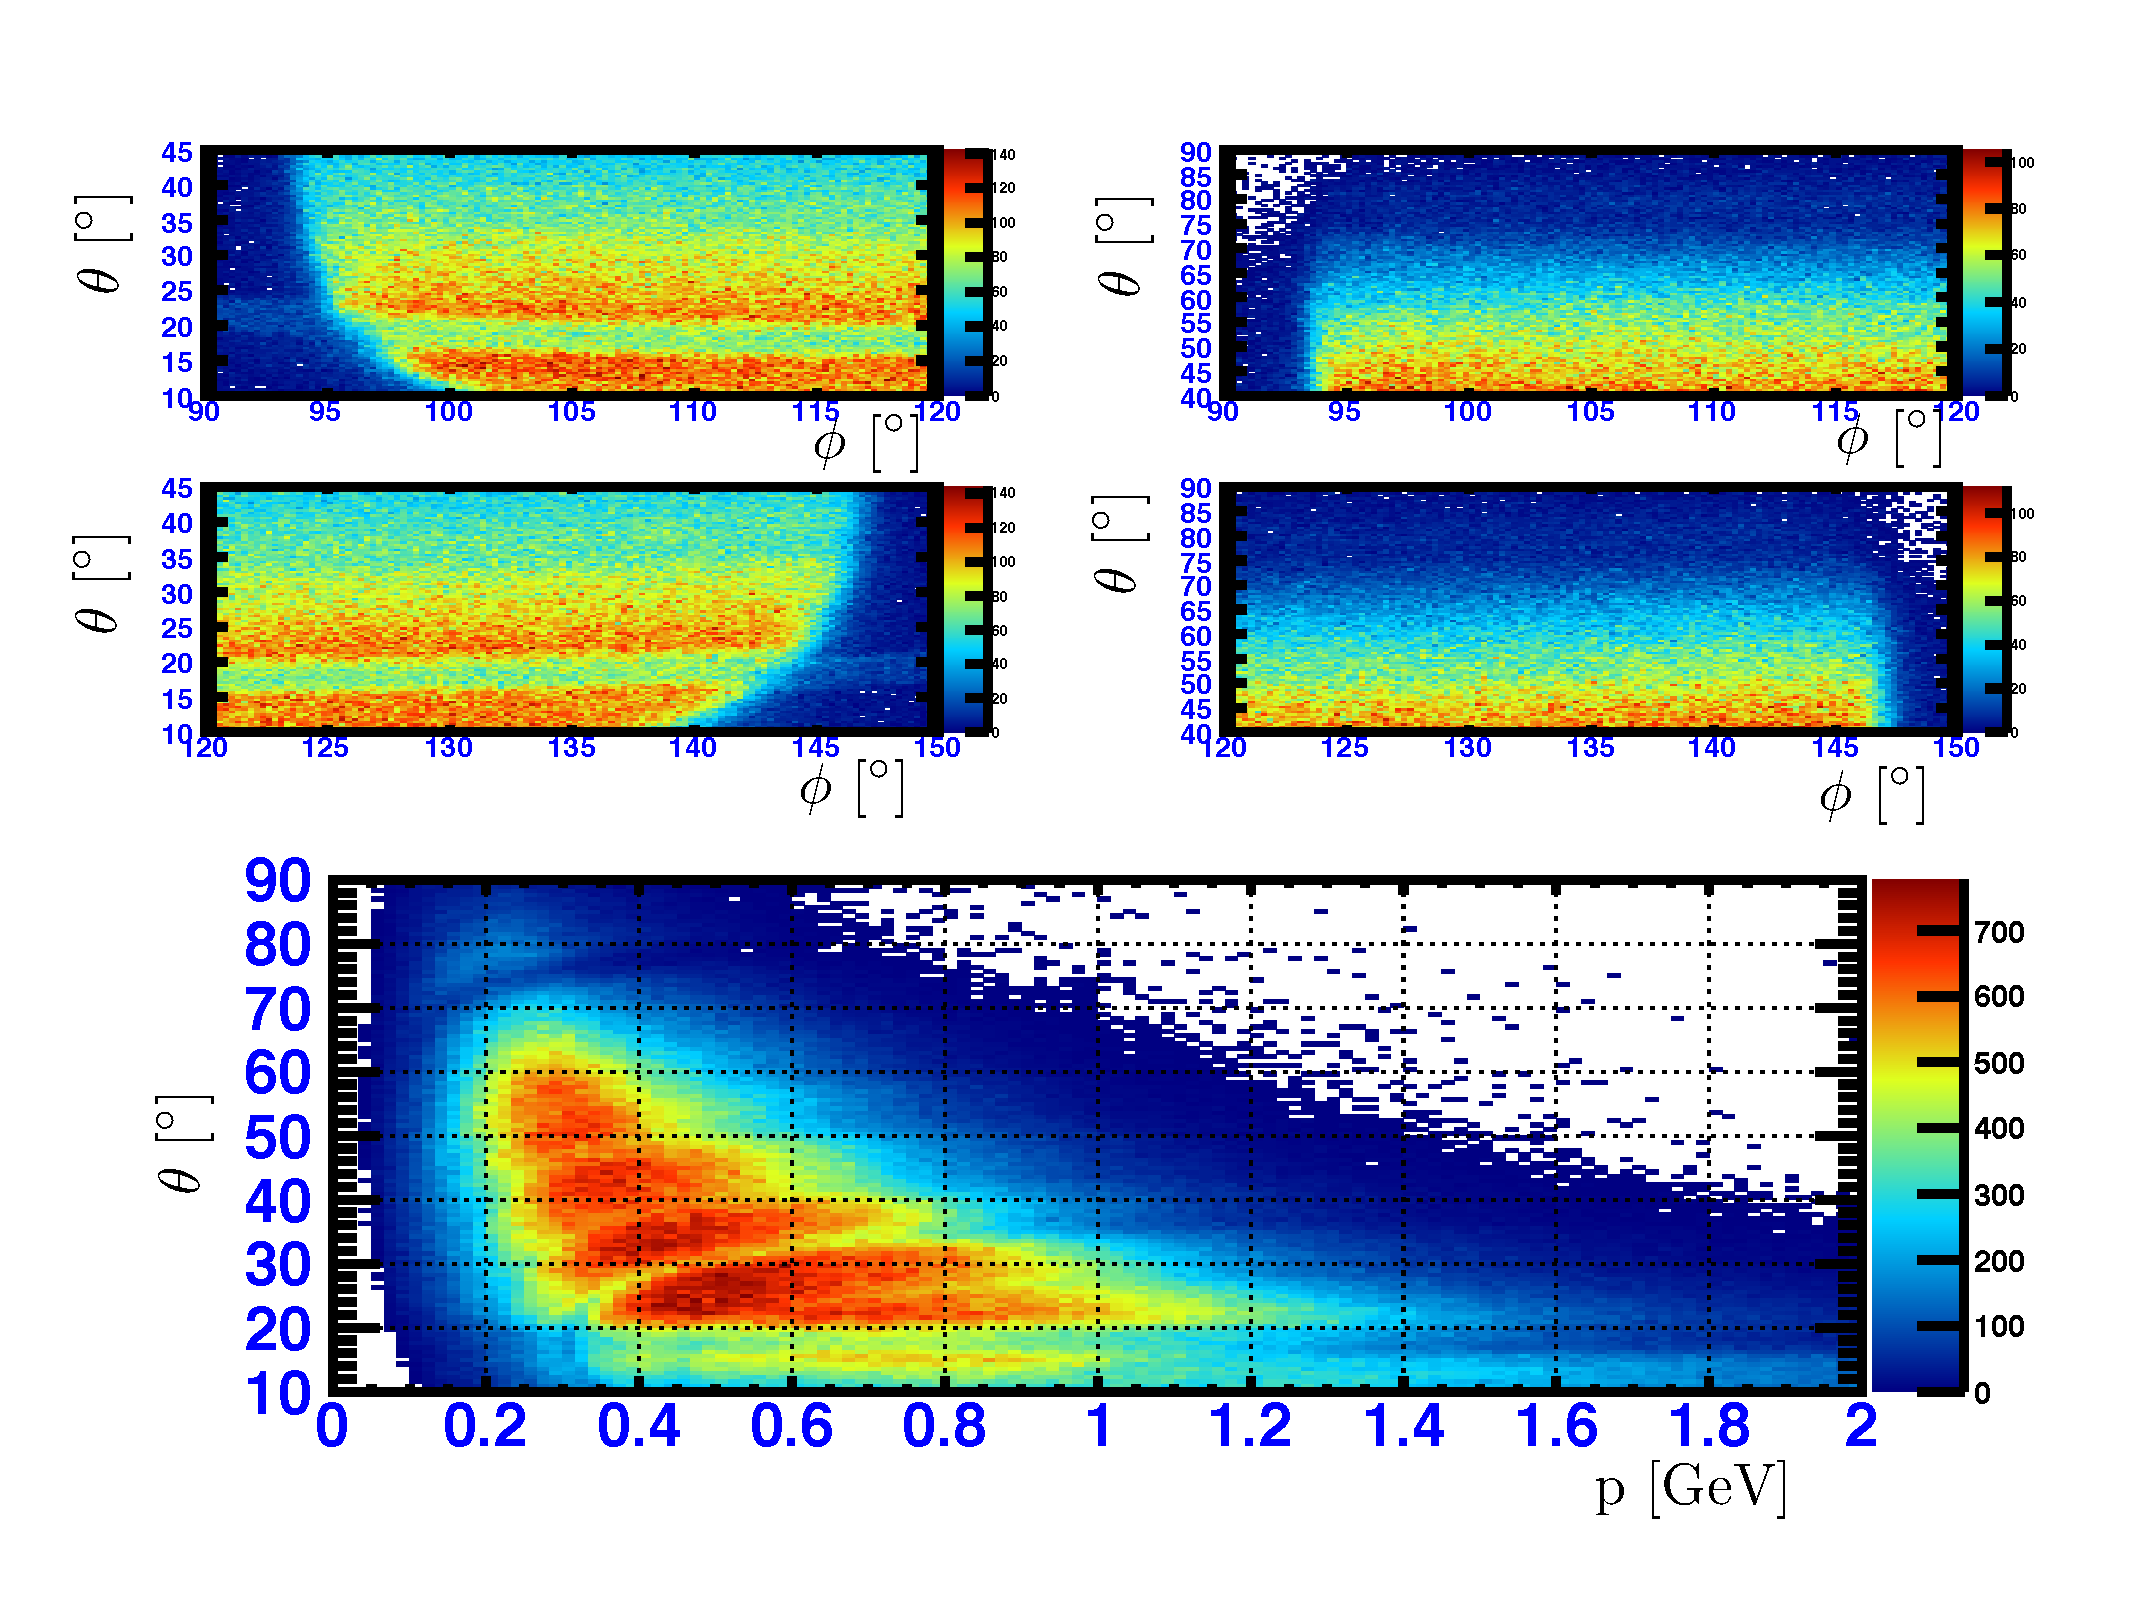
\includegraphics[width=\figwidth, height=3.5in,valign=c]{\grpath/analysis/FIDUCIAL_CUTS/TOF/RAW/pip_sec3.pdf}\label{fig:I_II}} \quad
  \\
  \subfloat[][]{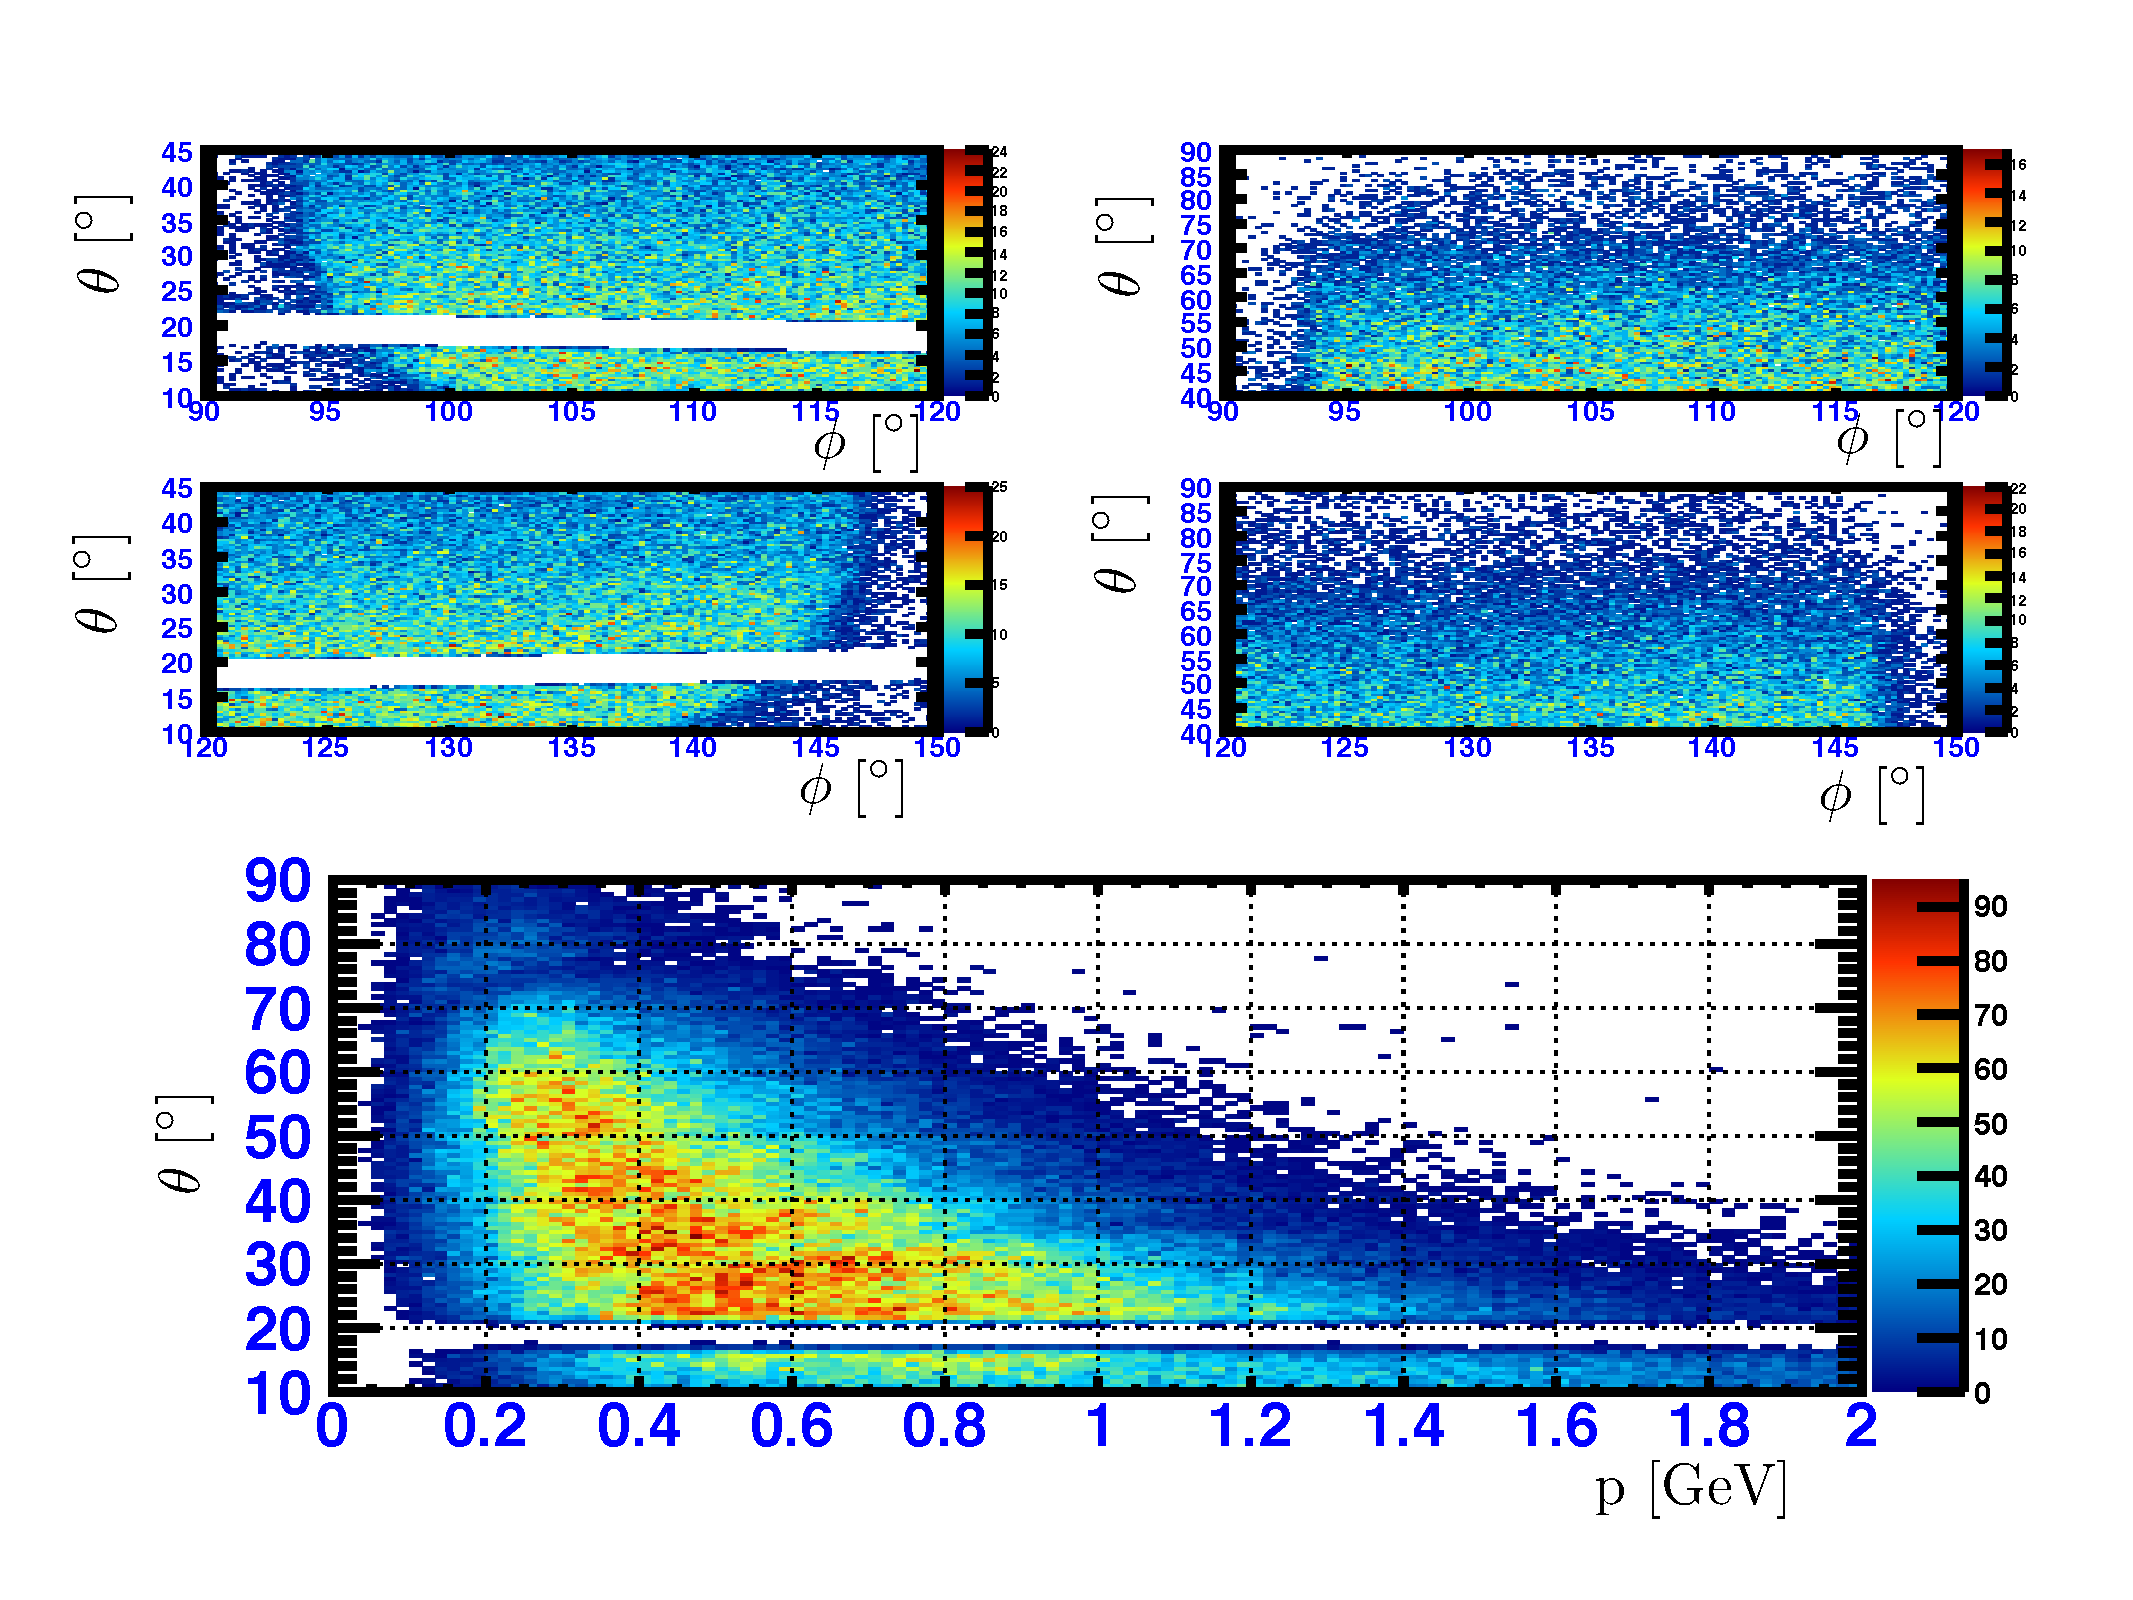
\includegraphics[width=\figwidth, height=3.5in,valign=c]{\grpath/analysis/FIDUCIAL_CUTS/TOF/KNOCK_OUT/pip_sec3_Knockout.pdf}\label{fig:II_II}} \\

      \caption {\abbr{TOF} inefficiency Plot for sector 3~(\ref{fig:I_II}). Inefficiency cut for $\pi^{+} \ $ and proton data ~(\ref{fig:II_II}). Notation same as in Fig.~\ref{fig:pos:tofcut_off}.}
        \label{fig:allI_II}
\end{figure}

\begin{figure}[!ht]
  \centering
  \subfloat[][]{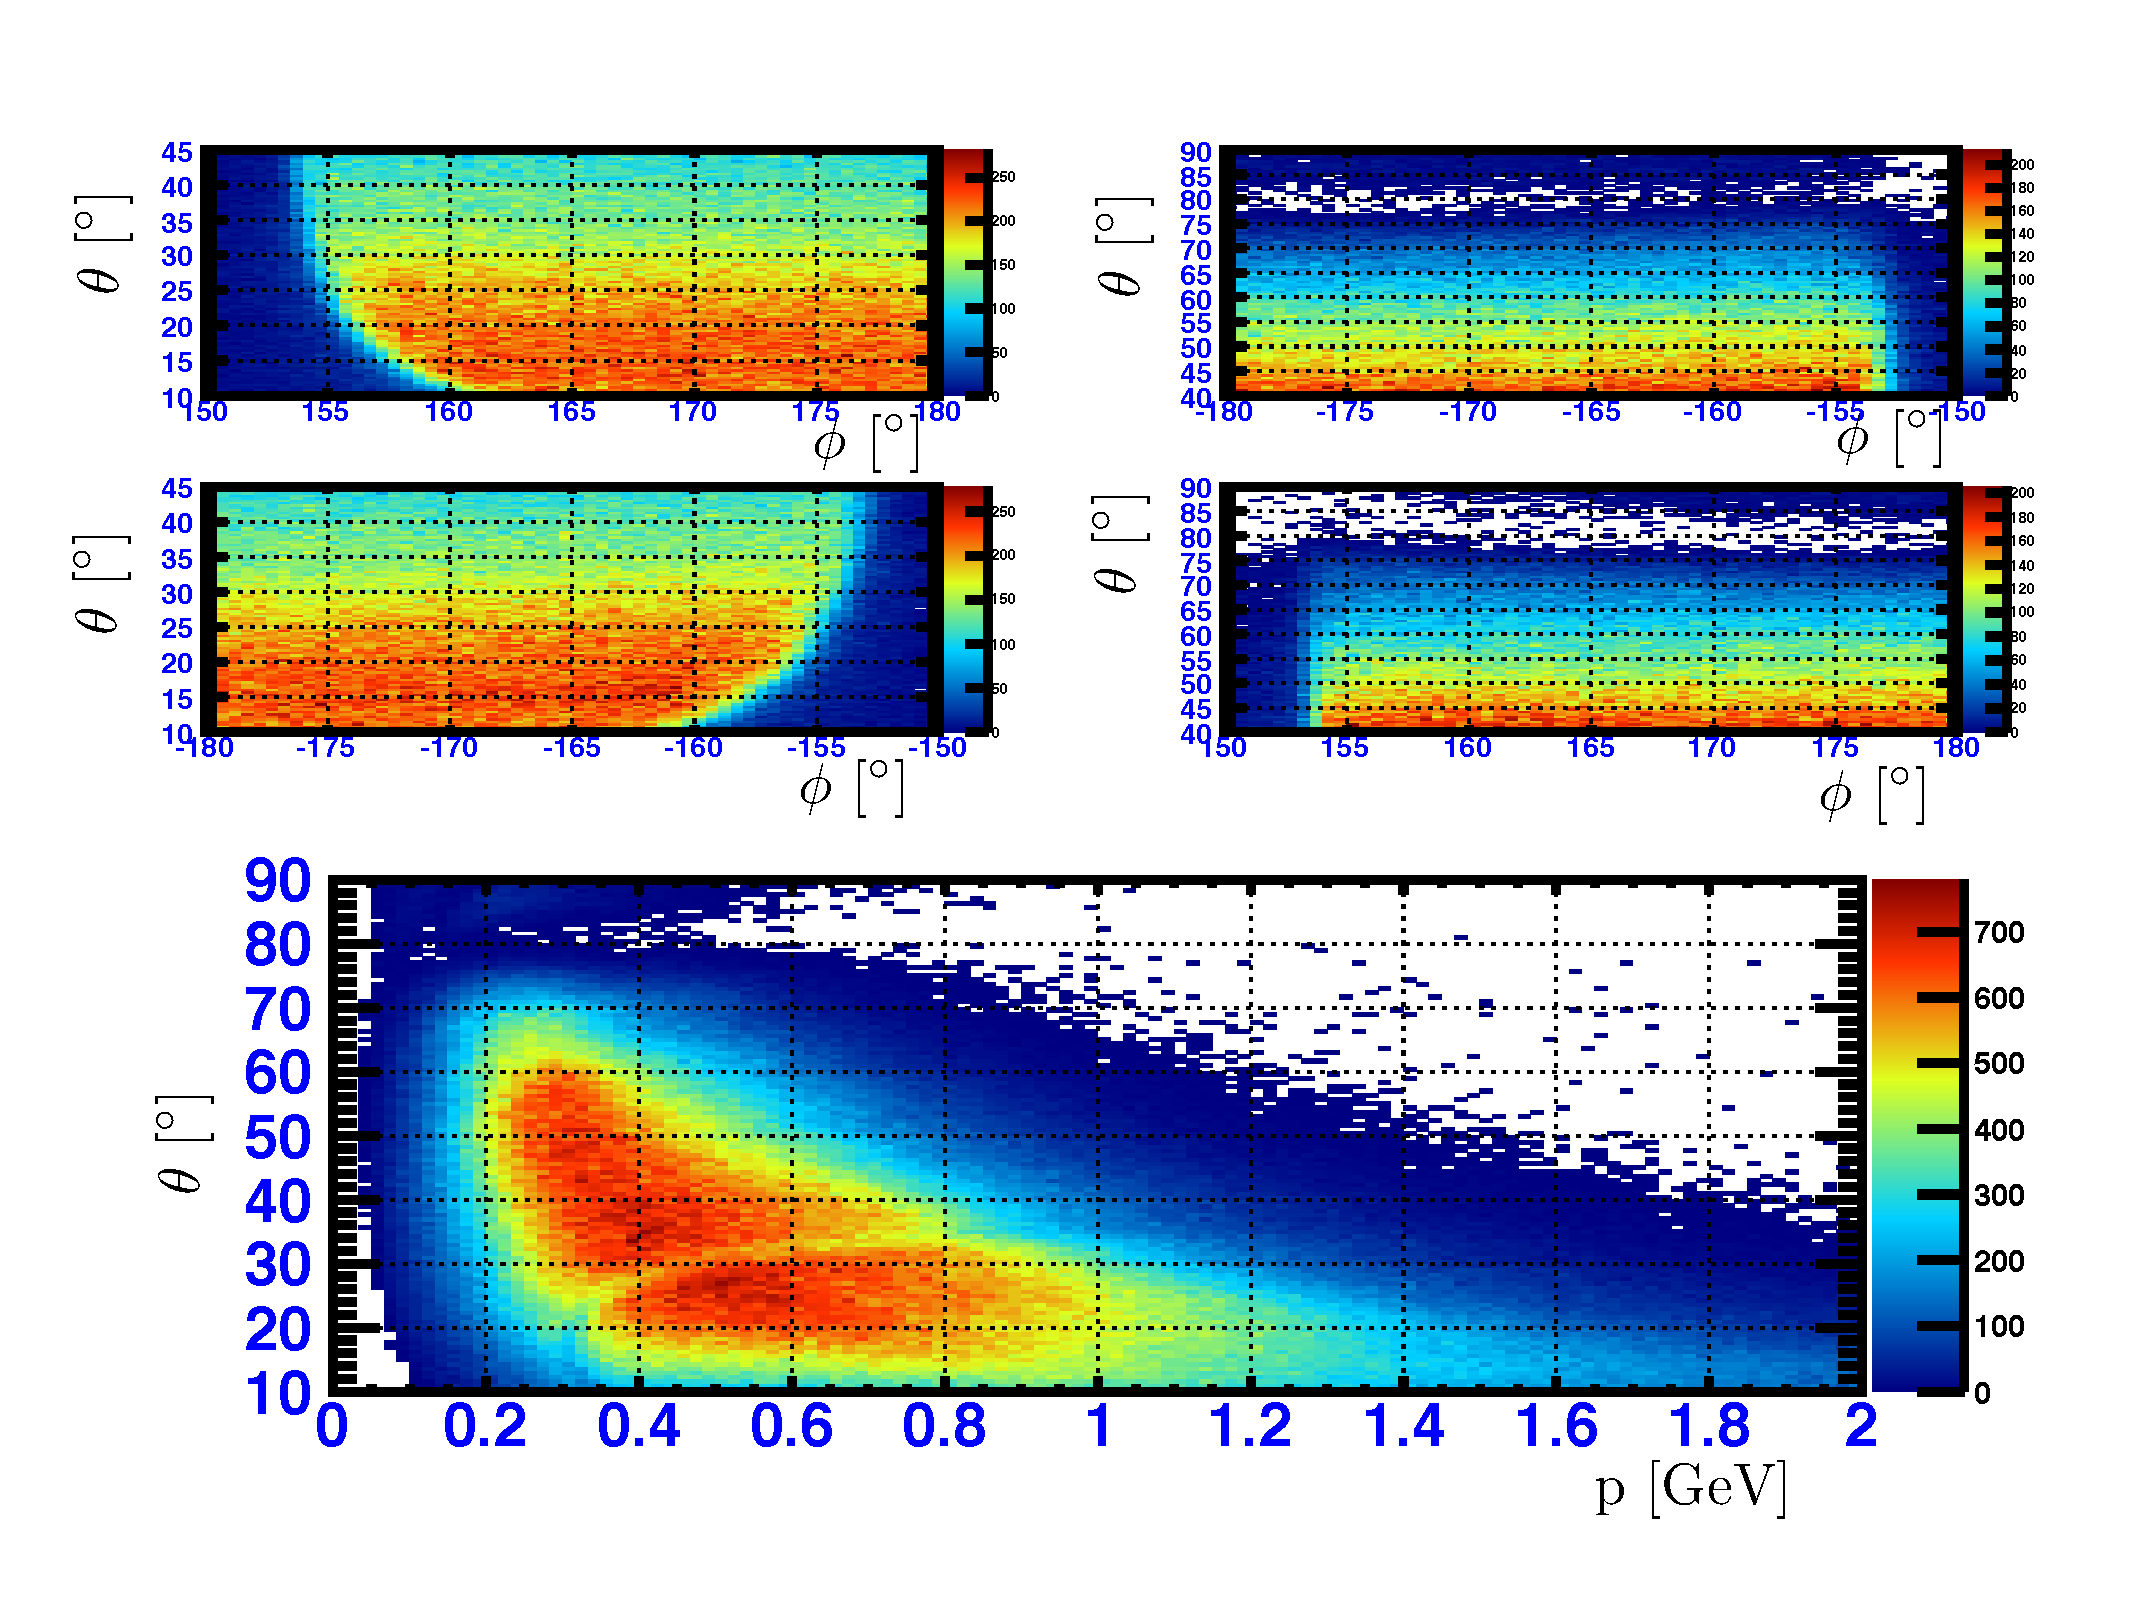
\includegraphics[width=\figwidth, height=3.5in,valign=c]{\grpath/analysis/FIDUCIAL_CUTS/TOF/RAW/pip_sec4.pdf}\label{fig:I_III}} \quad
  \\
  \subfloat[][]{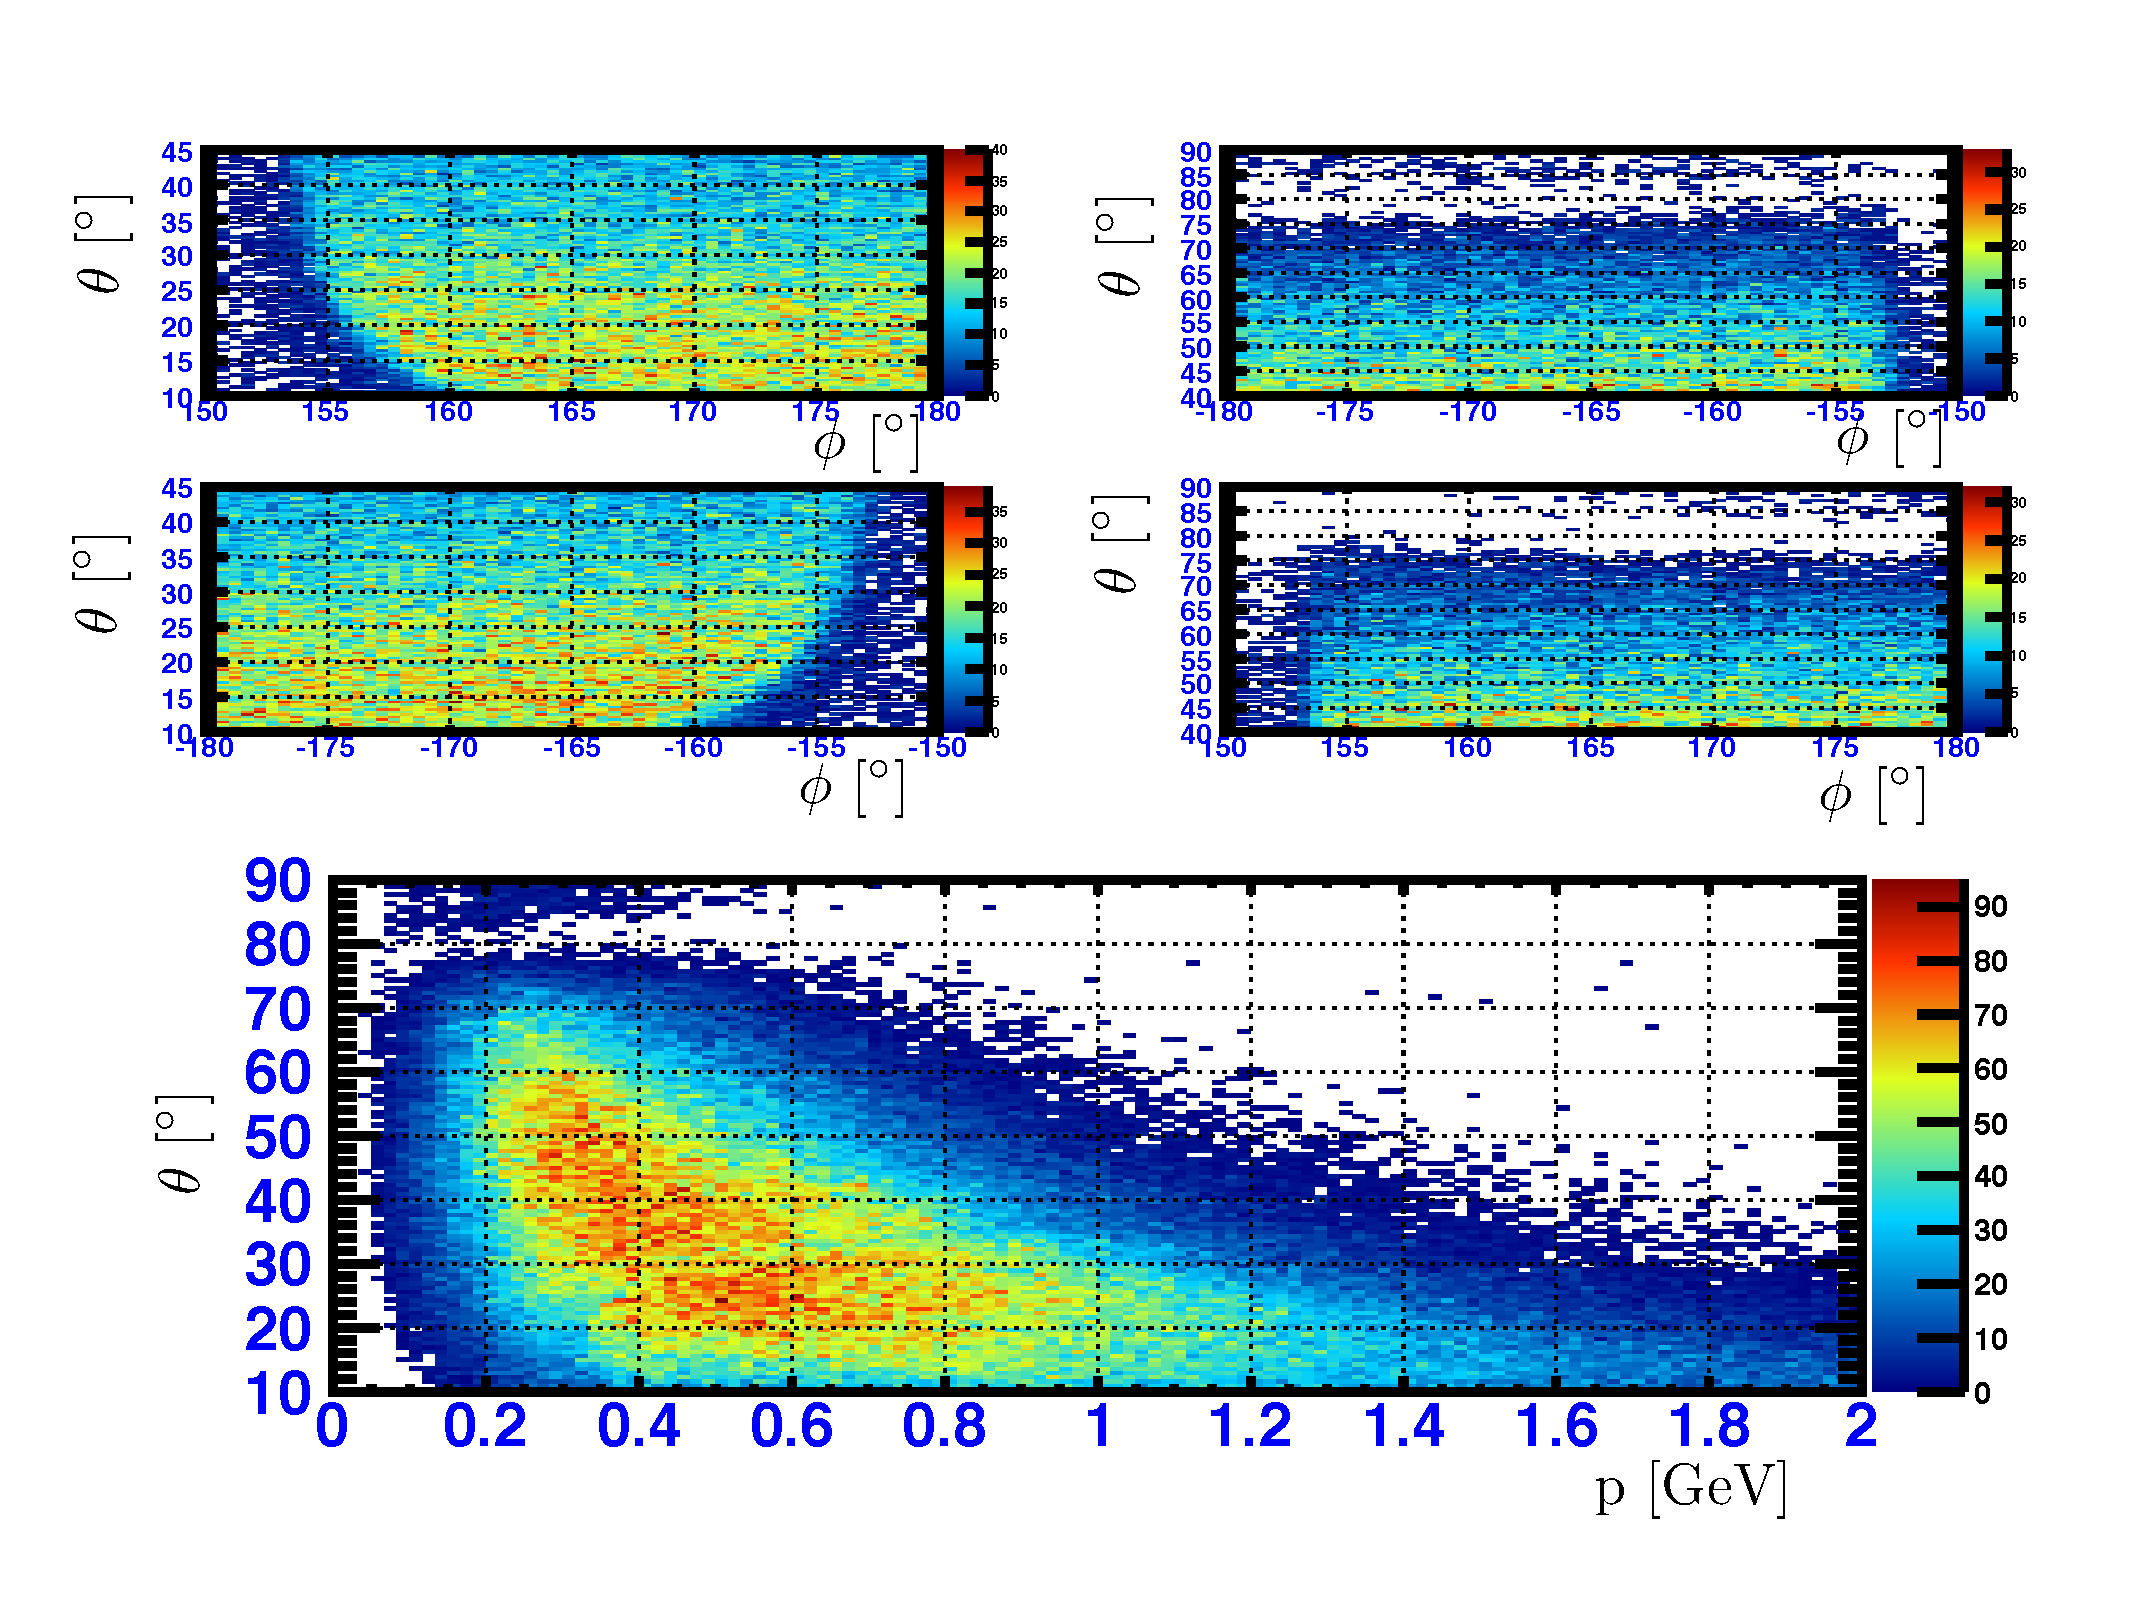
\includegraphics[width=\figwidth, height=3.5in,valign=c]{\grpath/analysis/FIDUCIAL_CUTS/TOF/KNOCK_OUT/pip_sec4_Knockout.pdf}\label{fig:II_III}} \\

      \caption {\abbr{TOF} inefficiency Plot for sector 4~(\ref{fig:I_III}). Inefficiency cut for $\pi^{+} \ $ and proton data ~(\ref{fig:II_III}). Notation same as in Fig.~\ref{fig:pos:tofcut_off}.}
        \label{fig:allI_III}
\end{figure}

\begin{figure}[!ht]
  \centering
  \subfloat[][]{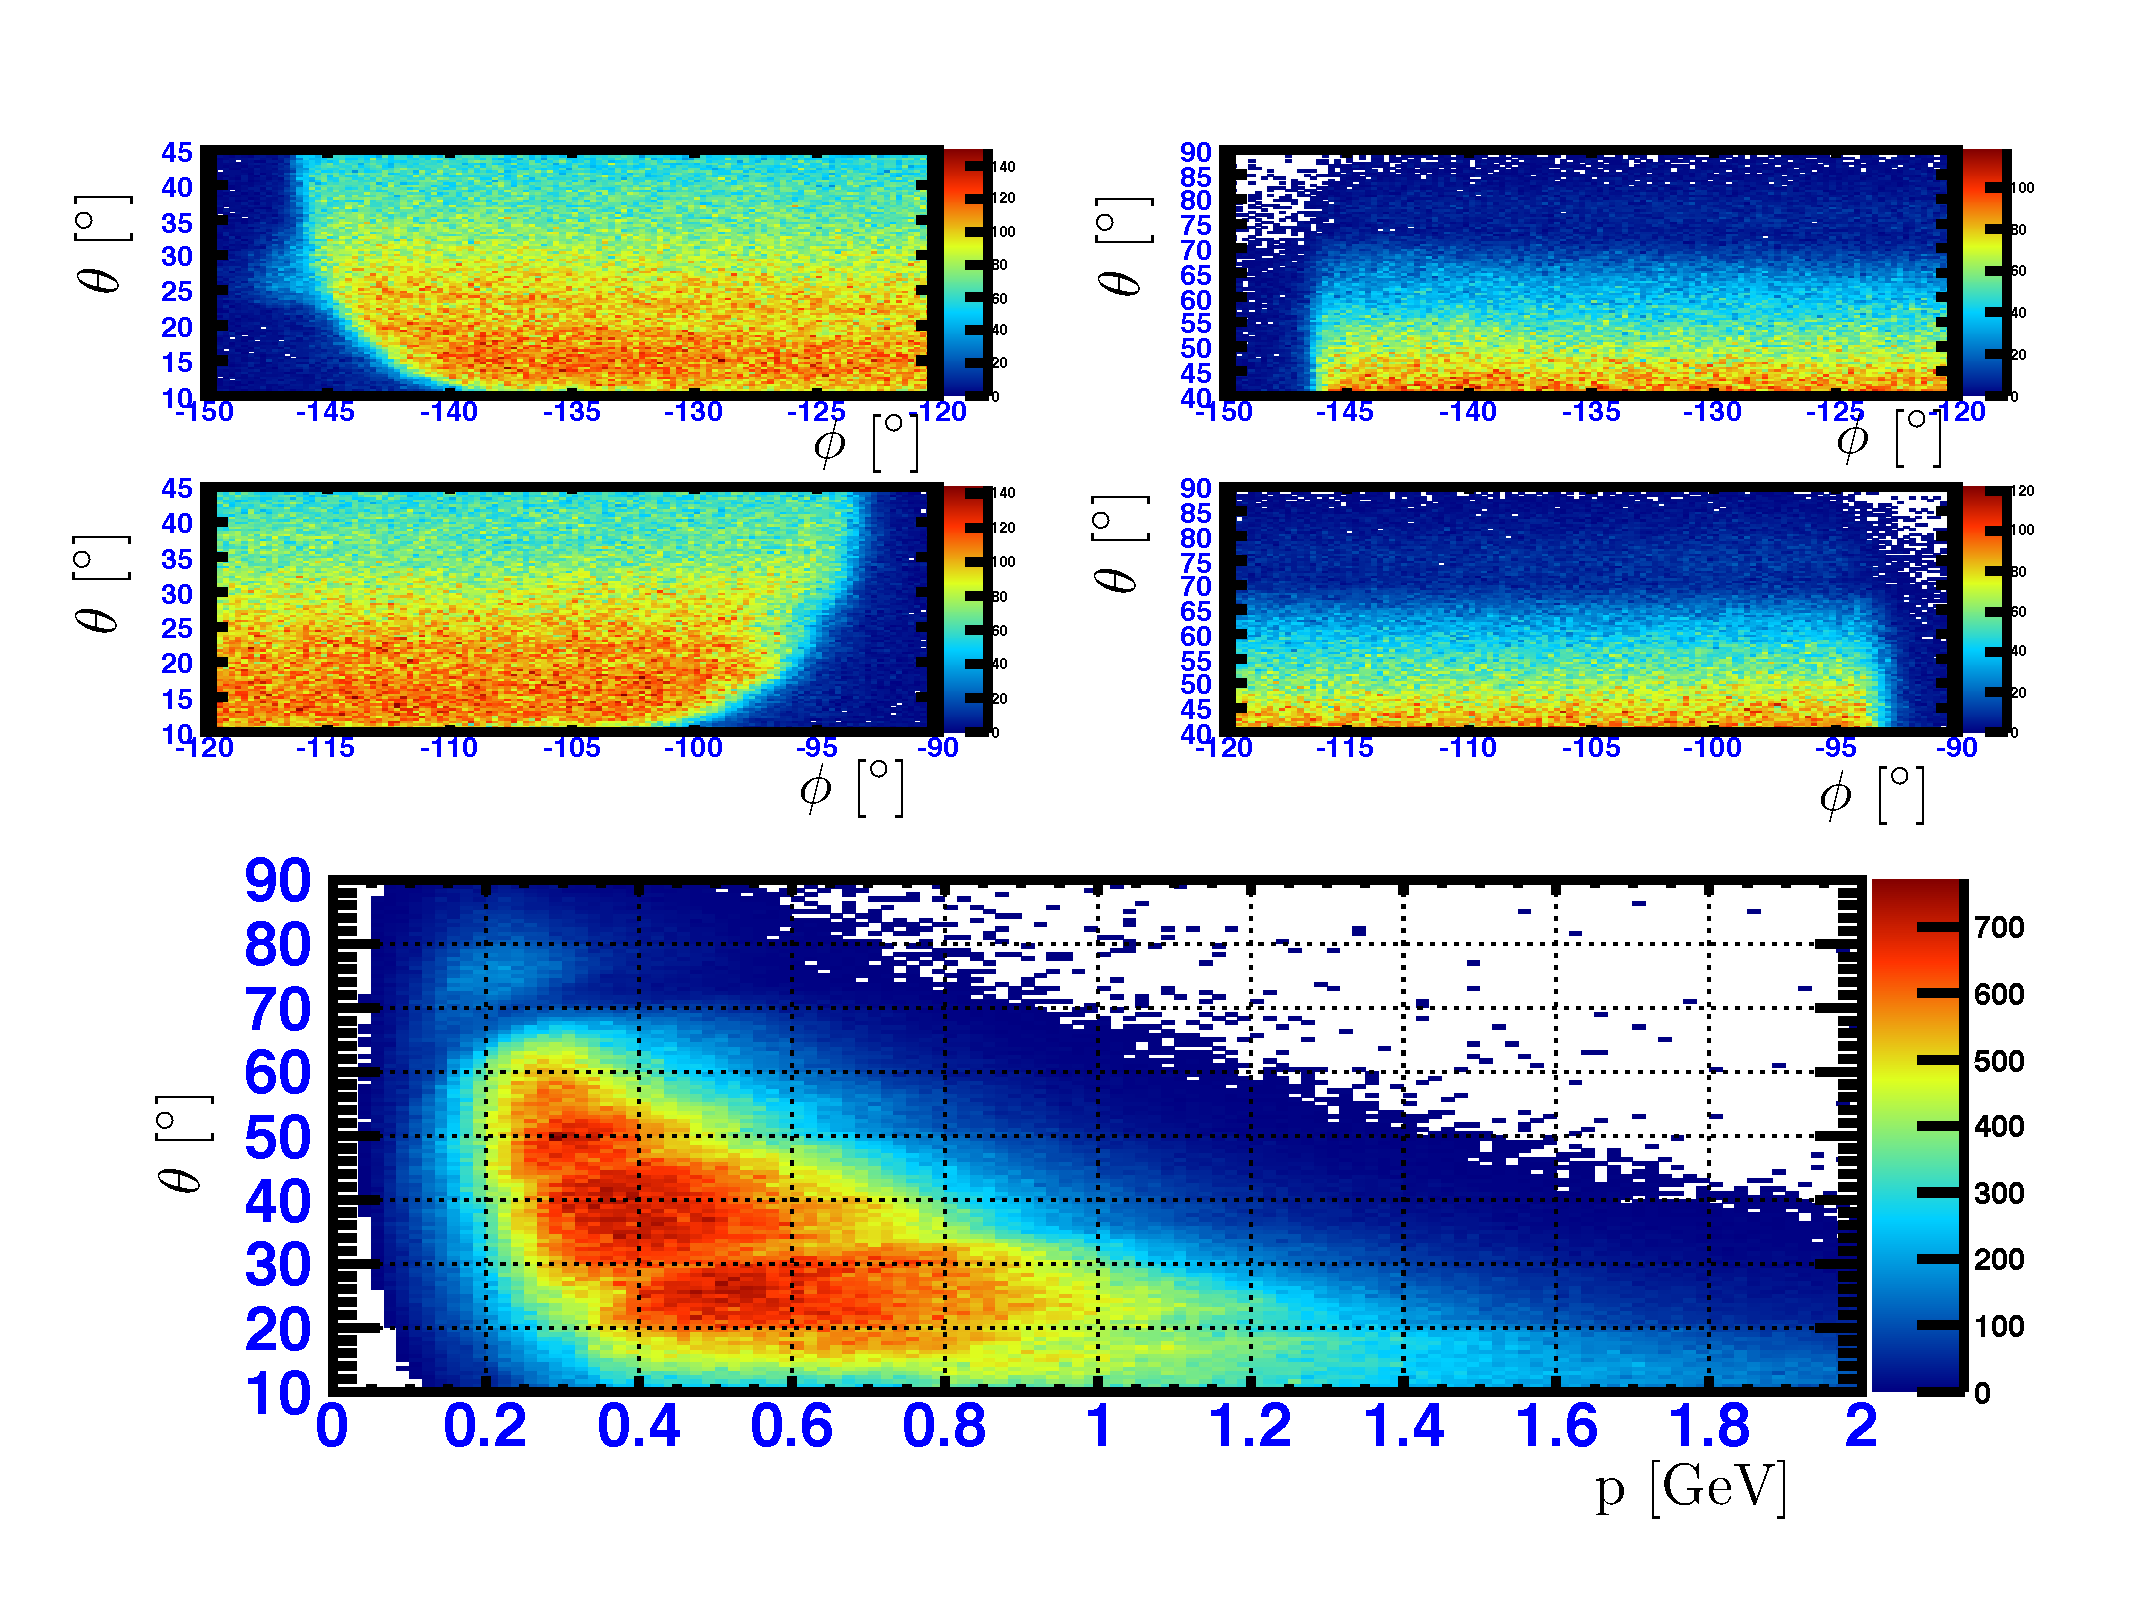
\includegraphics[width=\figwidth, height=3.5in,valign=c]{\grpath/analysis/FIDUCIAL_CUTS/TOF/RAW/pip_sec5.pdf}\label{fig:I_IIII}} \quad
  \\
  \subfloat[][]{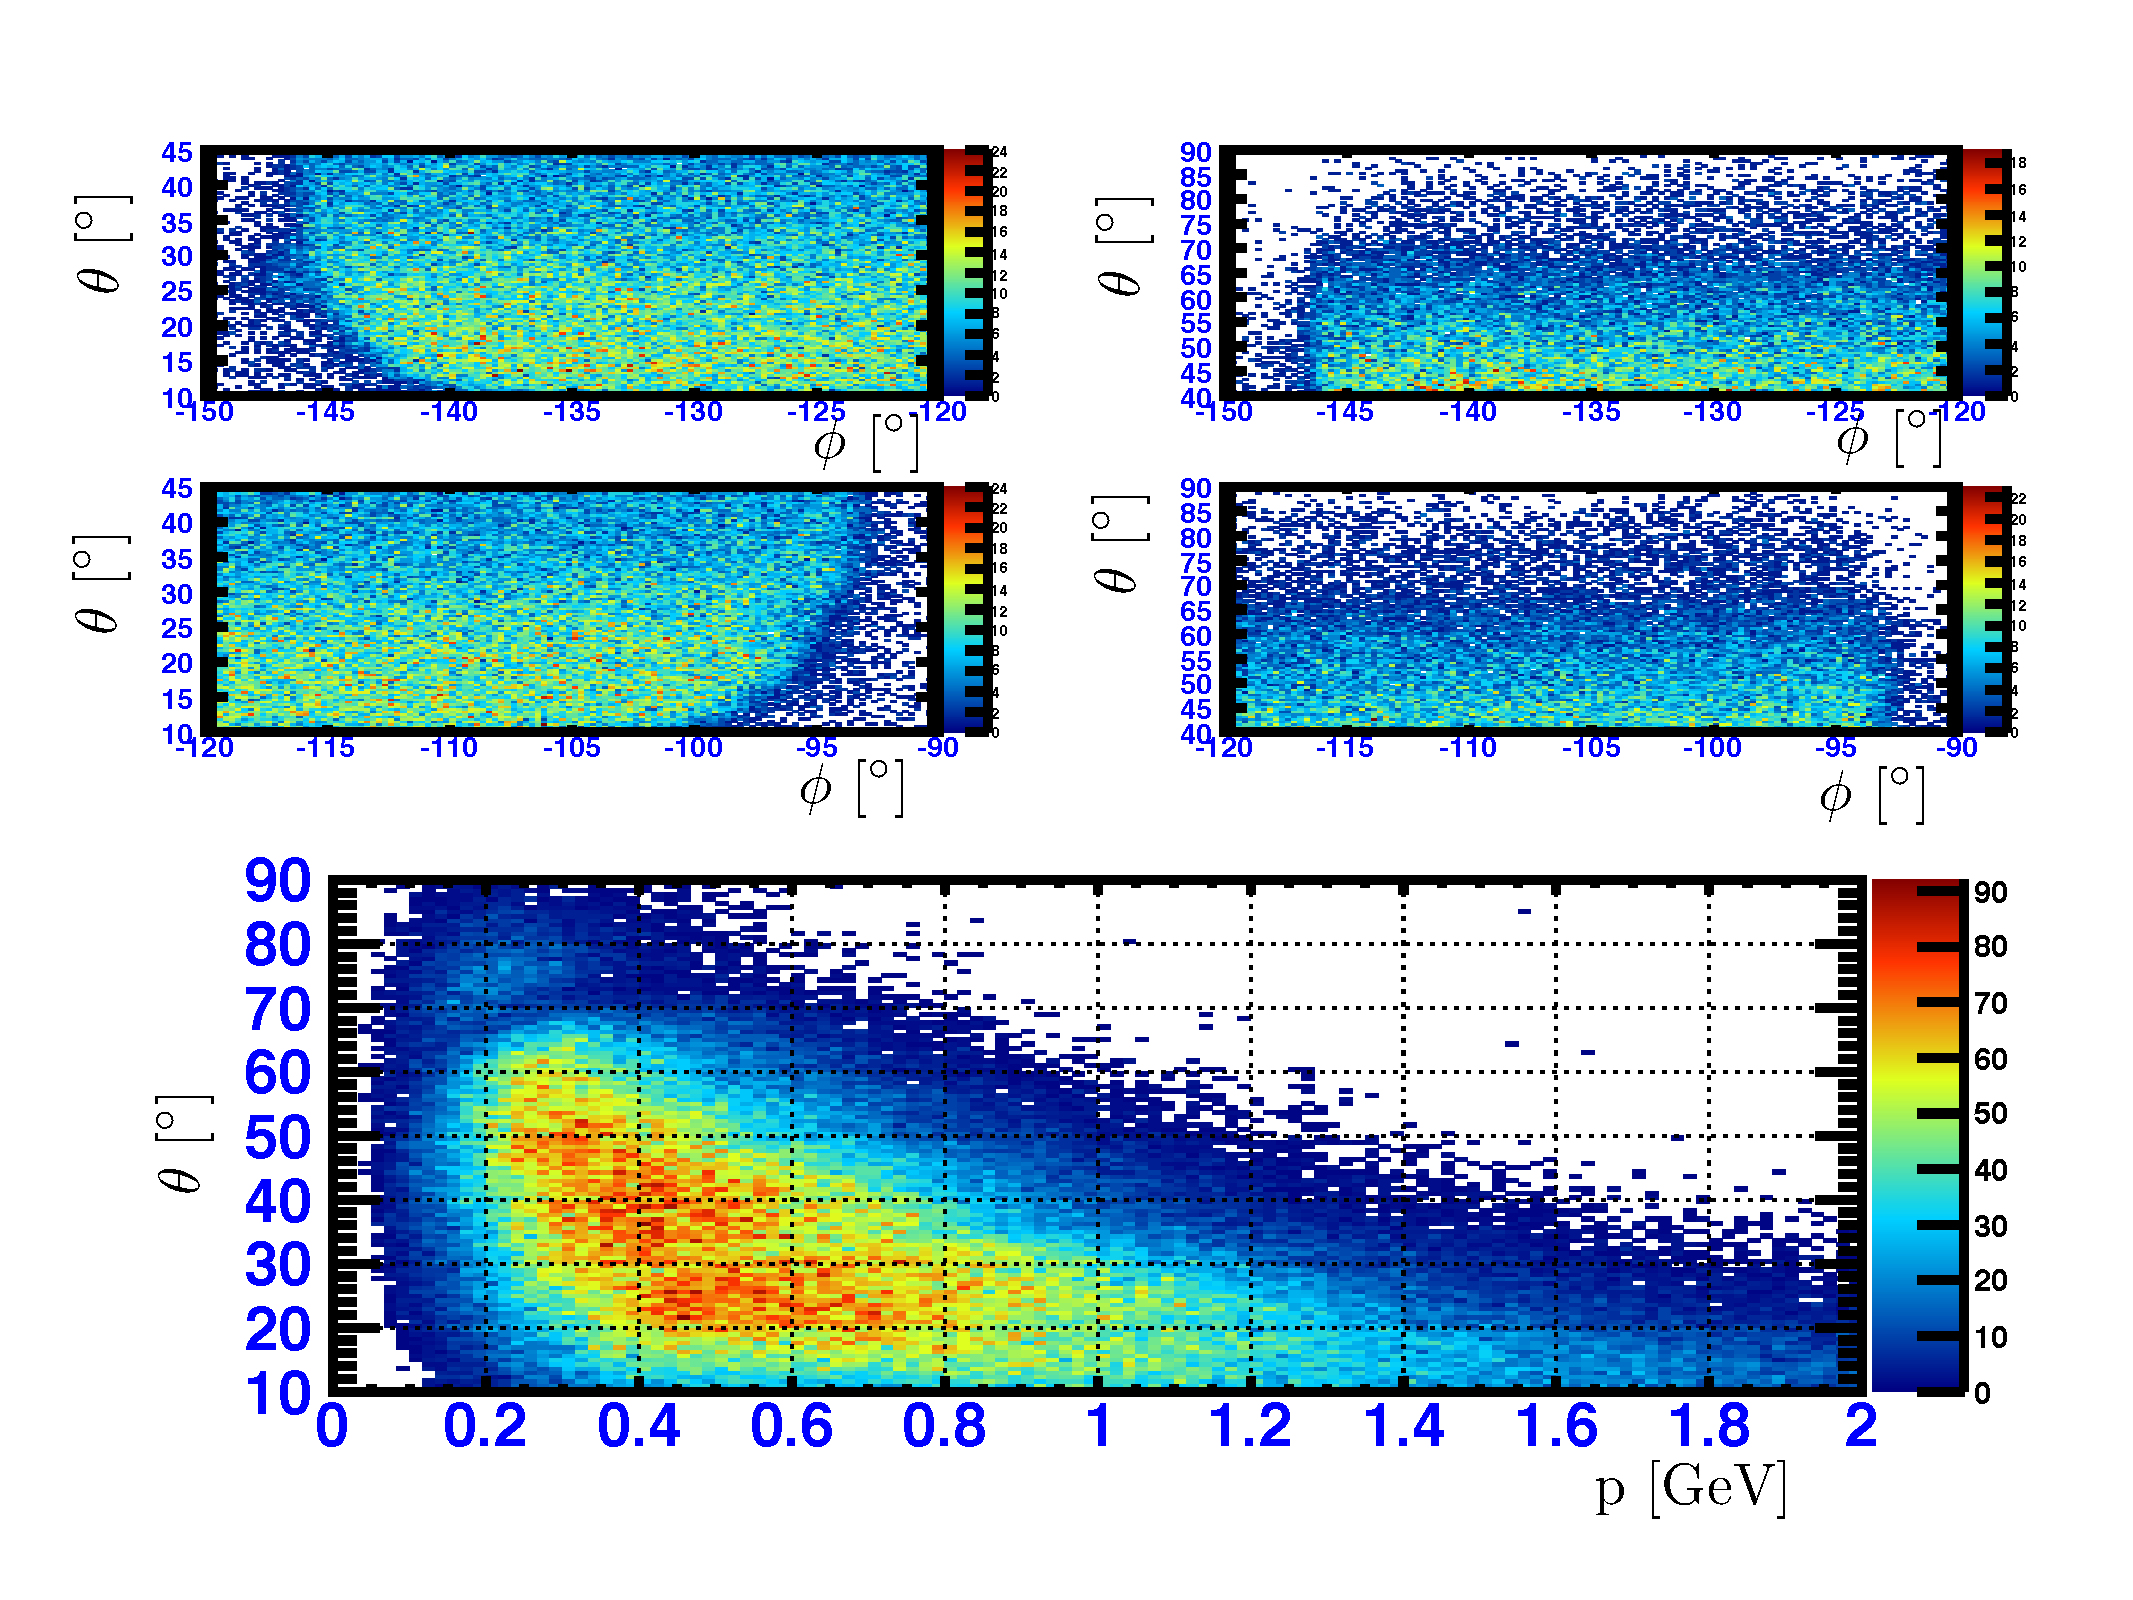
\includegraphics[width=\figwidth, height=3.5in,valign=c]{\grpath/analysis/FIDUCIAL_CUTS/TOF/KNOCK_OUT/pip_sec5_Knockout.pdf}\label{fig:II_IIII}} \\

      \caption {\abbr{TOF} inefficiency Plot for sector 5~(\ref{fig:I_IIII}). Inefficiency cut for $\pi^{+} \ $ and proton data ~(\ref{fig:II_IIII}). Notation same as in Fig.~\ref{fig:pos:tofcut_off}.}
        \label{fig:allI_IIII}
\end{figure}

\begin{figure}[!ht]
  \centering
  \subfloat[][]{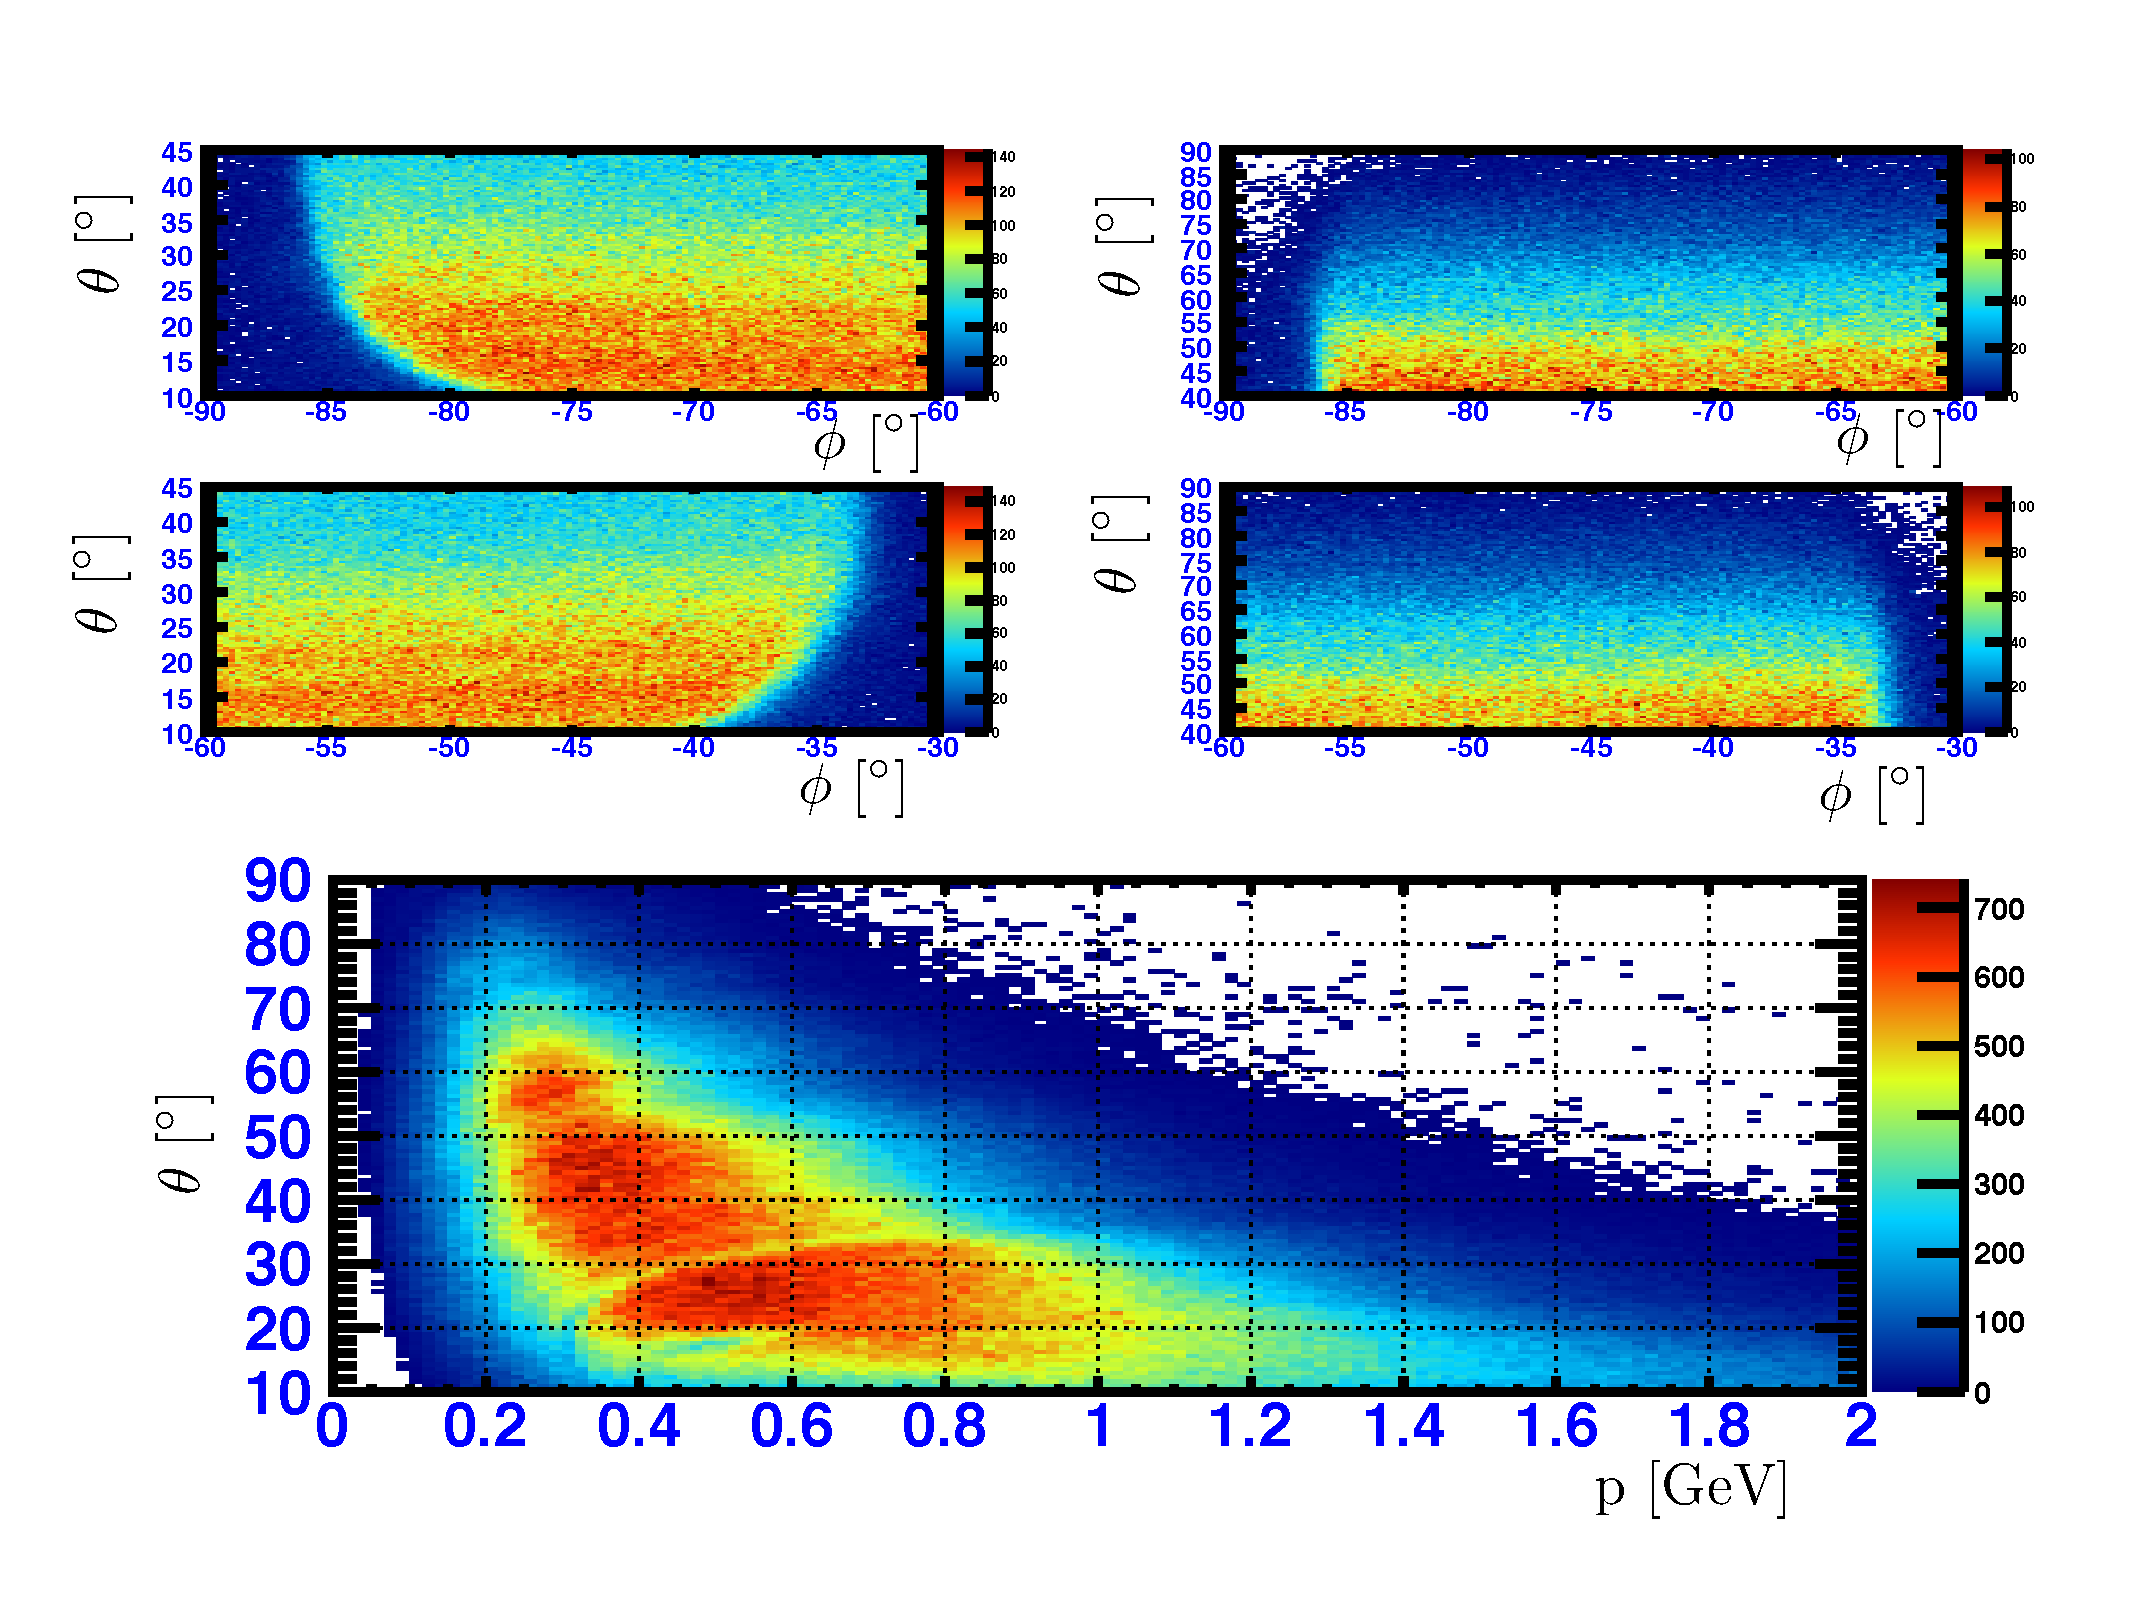
\includegraphics[width=\figwidth, height=3.5in,valign=c]{\grpath/analysis/FIDUCIAL_CUTS/TOF/RAW/pip_sec6.pdf}\label{fig:I_IV}} \quad
  \\
  \subfloat[][]{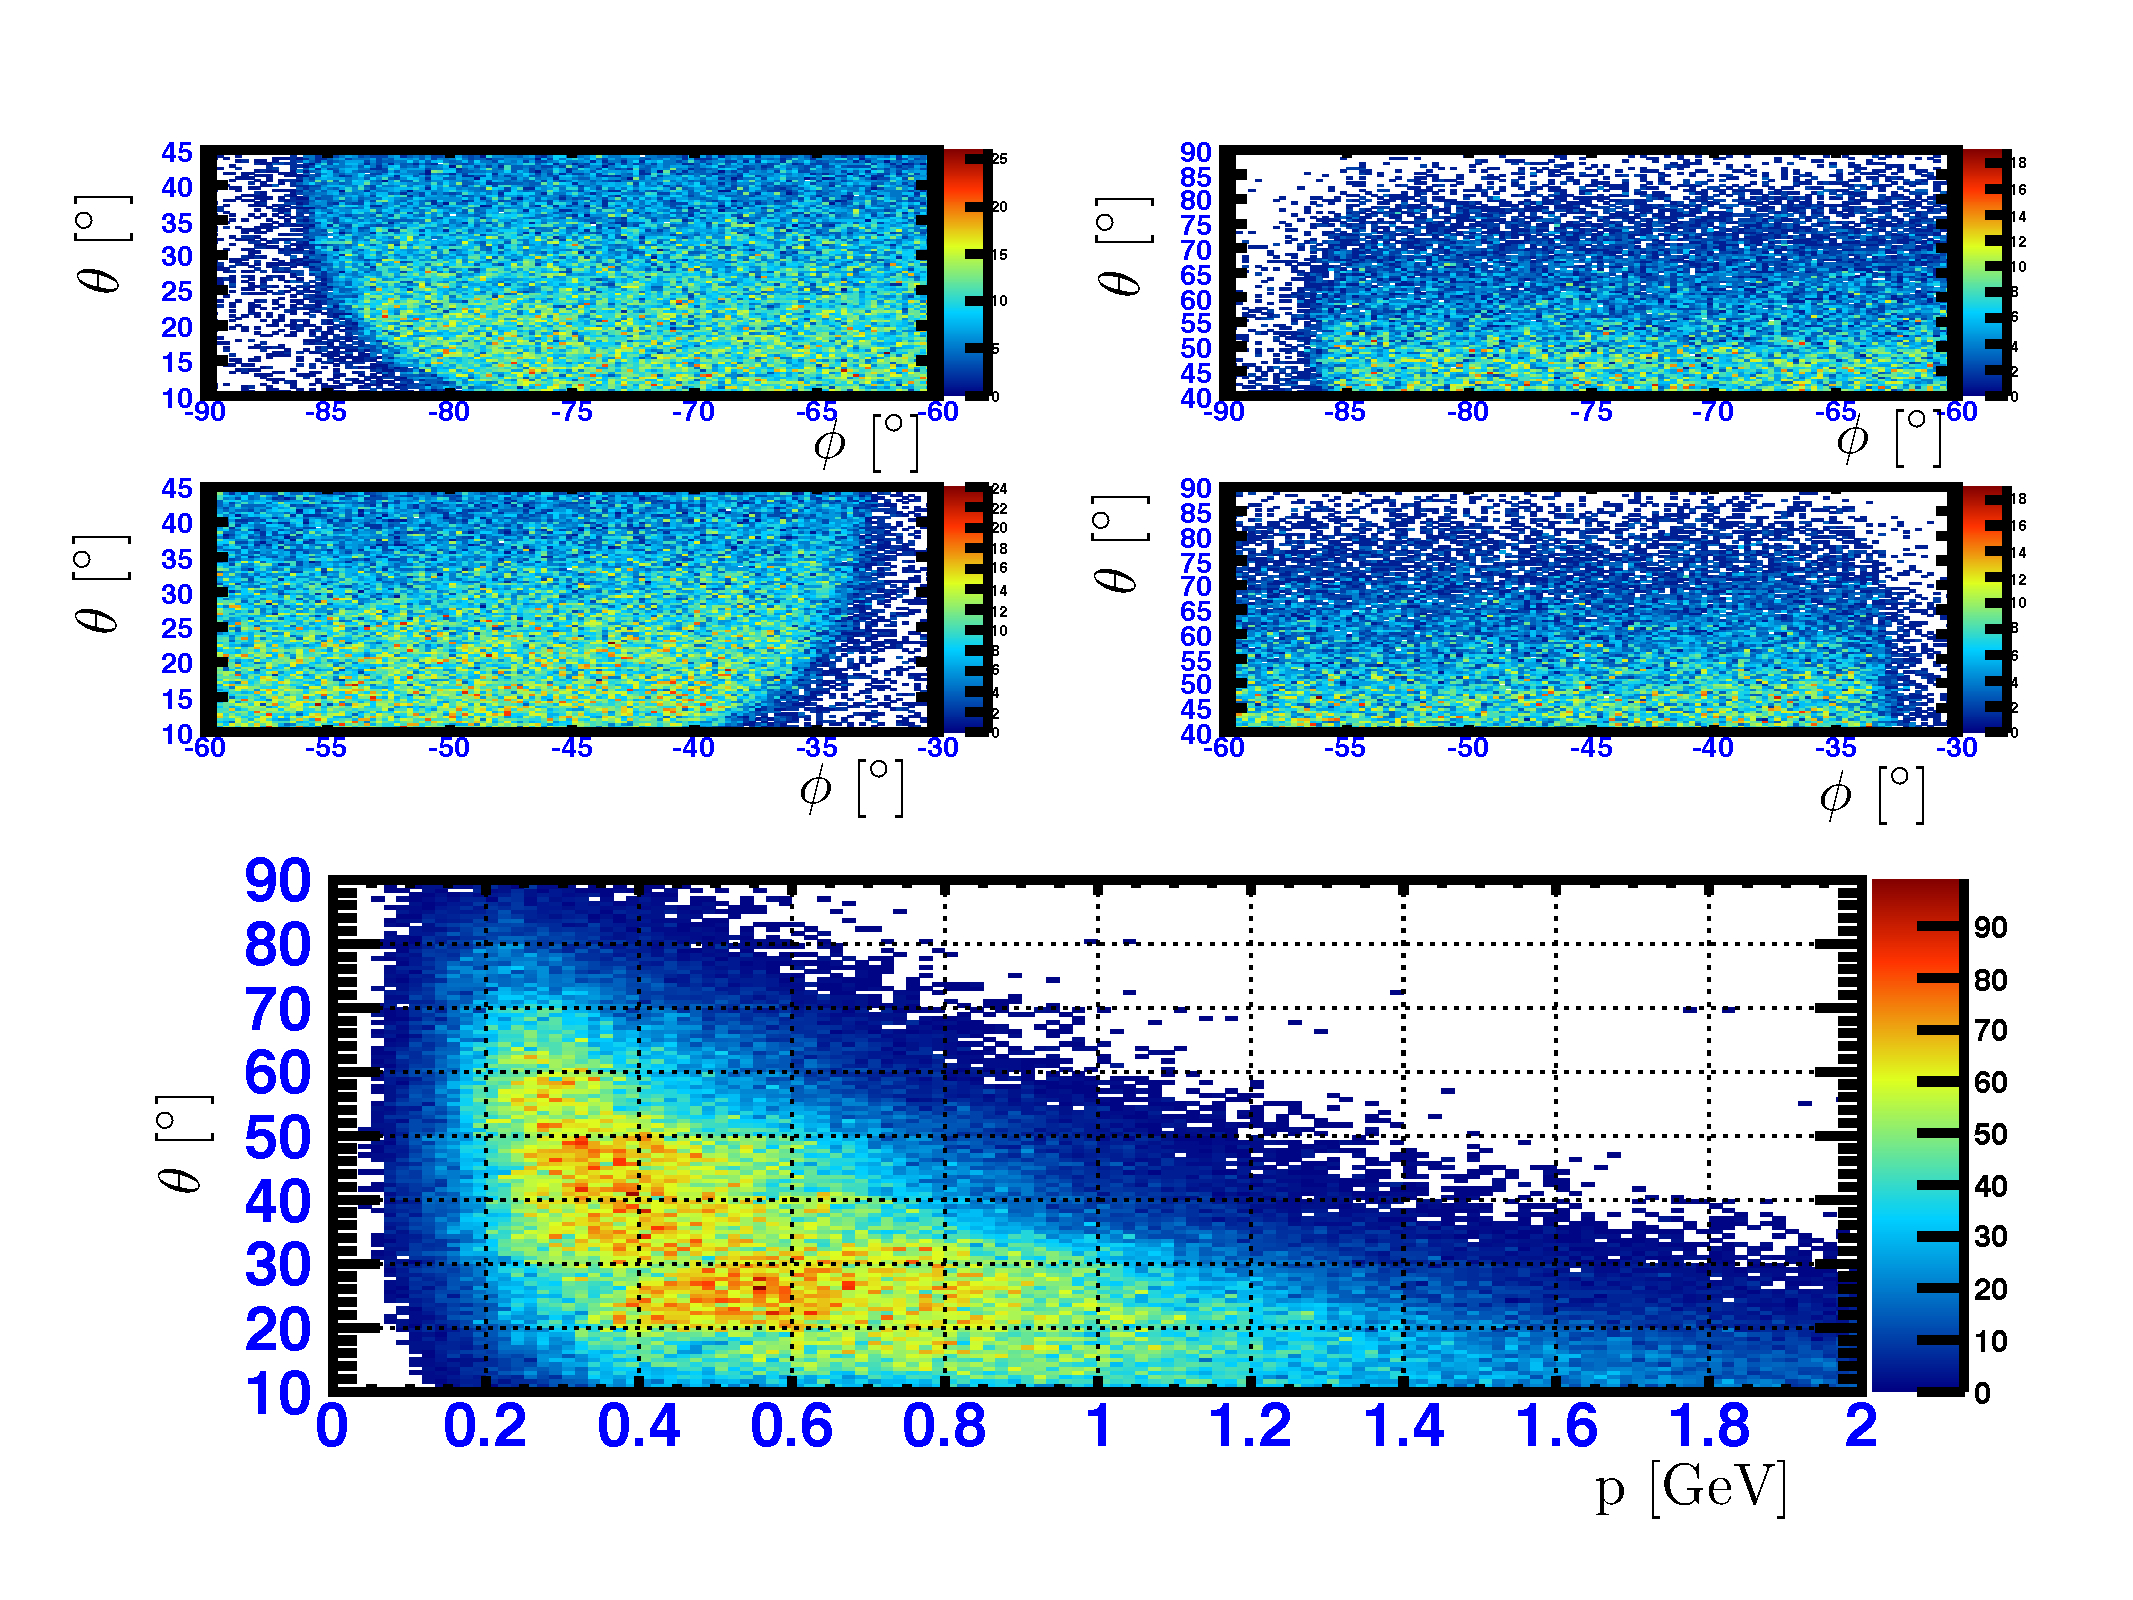
\includegraphics[width=\figwidth, height=3.5in,valign=c]{\grpath/analysis/FIDUCIAL_CUTS/TOF/KNOCK_OUT/pip_sec6_Knockout.pdf}\label{fig:II_IV}} \\

      \caption {\abbr{TOF} inefficiency Plot for sector 6~(\ref{fig:I_IV}). Inefficiency cut for $\pi^{+} \ $ and proton data ~(\ref{fig:II_IV}). Notation same as in Fig.~\ref{fig:pos:tofcut_off}.}
        \label{fig:allI_IV}
\end{figure}



\FloatBarrier 


\section{\abbr{EC} Inefficiency Study}
Sec.~\ref{sec:analysis.eccc_fid} refers to this section for a complete view of the \abbr{EC} study performed. All inefficiencies and cuts shown are for he $e^-$ data. These inefficiencies and cuts are valid for the $e^+$ data.


% % % %SECTOR 1
\begin{figure}[!ht]
  \centering
  \subfloat[][]{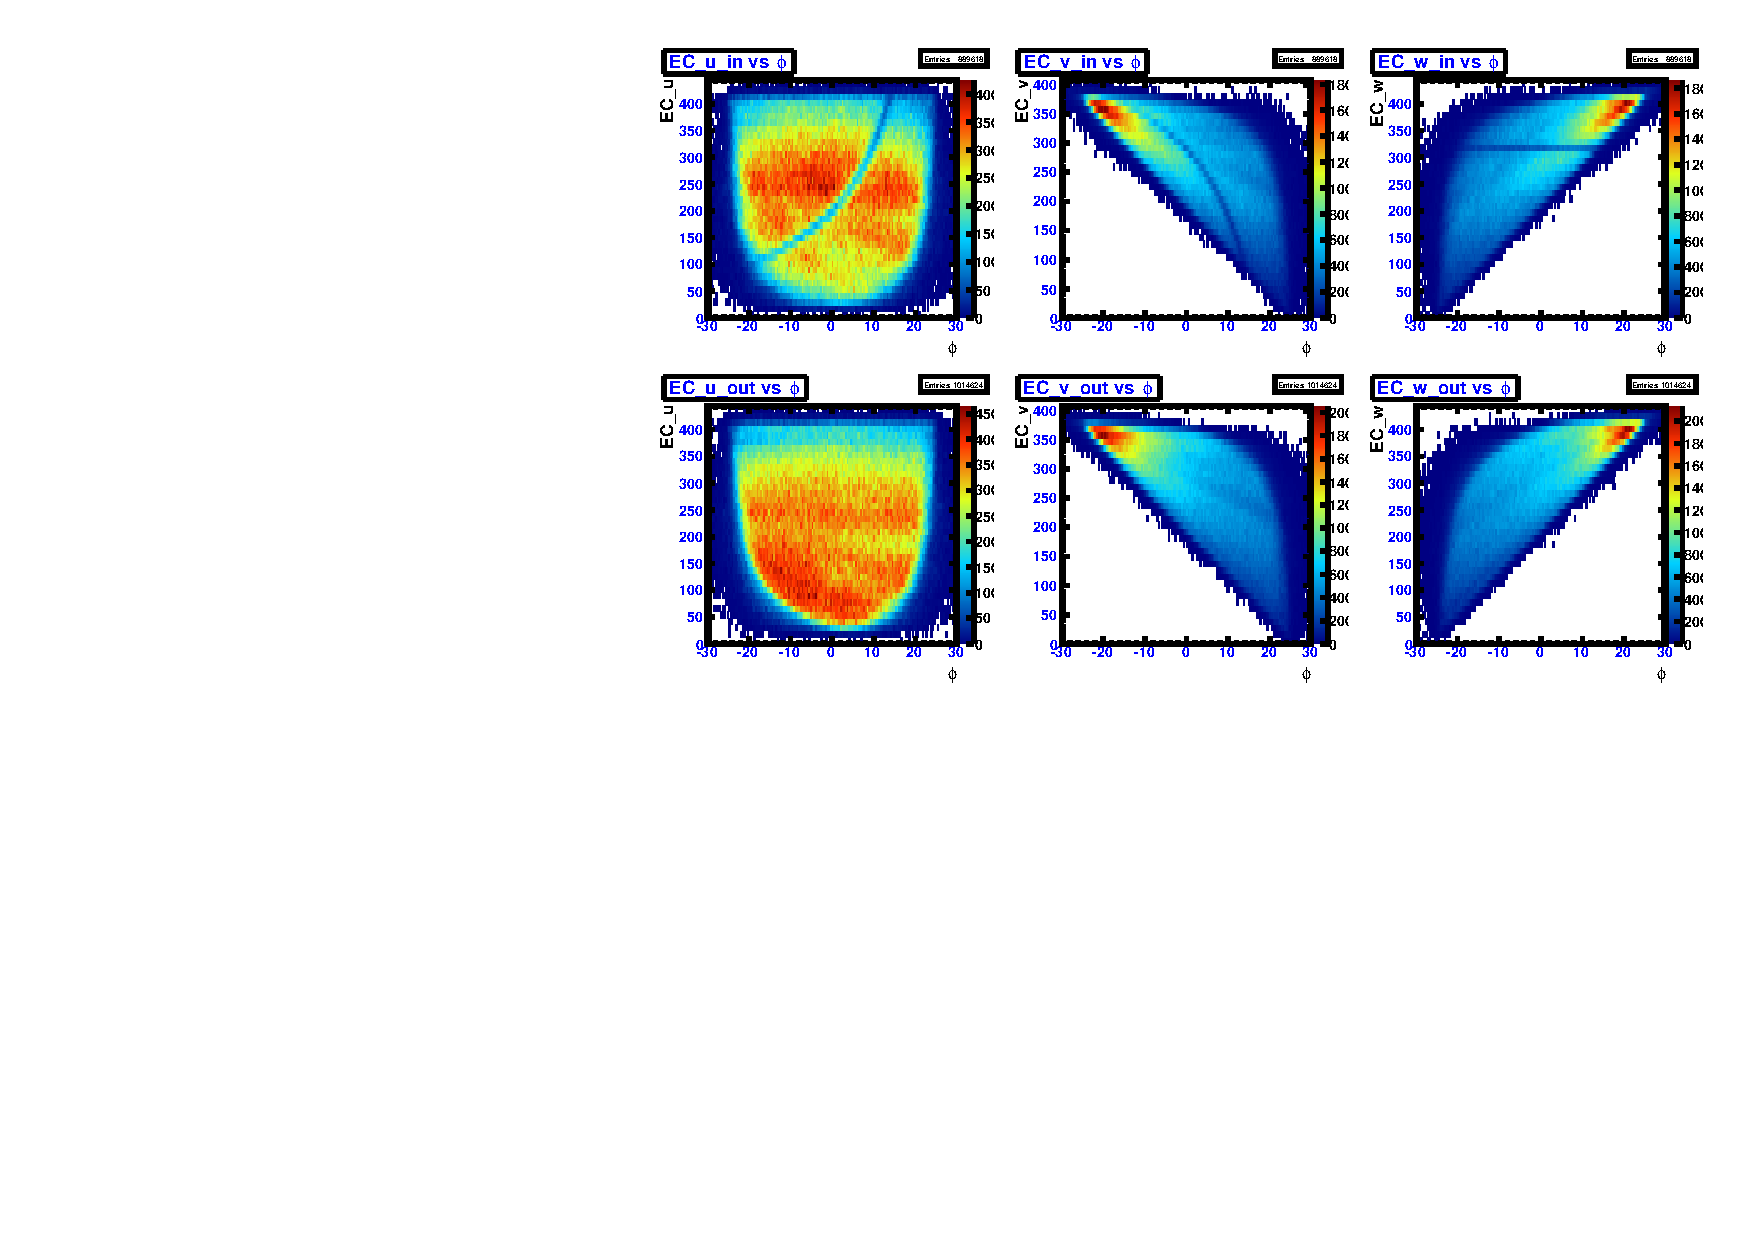
\includegraphics[width=\figwidth, height=3.5in,valign=c]{\grpath/analysis/FIDUCIAL_CUTS/EC/pim_ecuvw_phi_NOKnockout_sec1.pdf}\label{fig:EC_I_I}} \quad
  \\
  \subfloat[][]{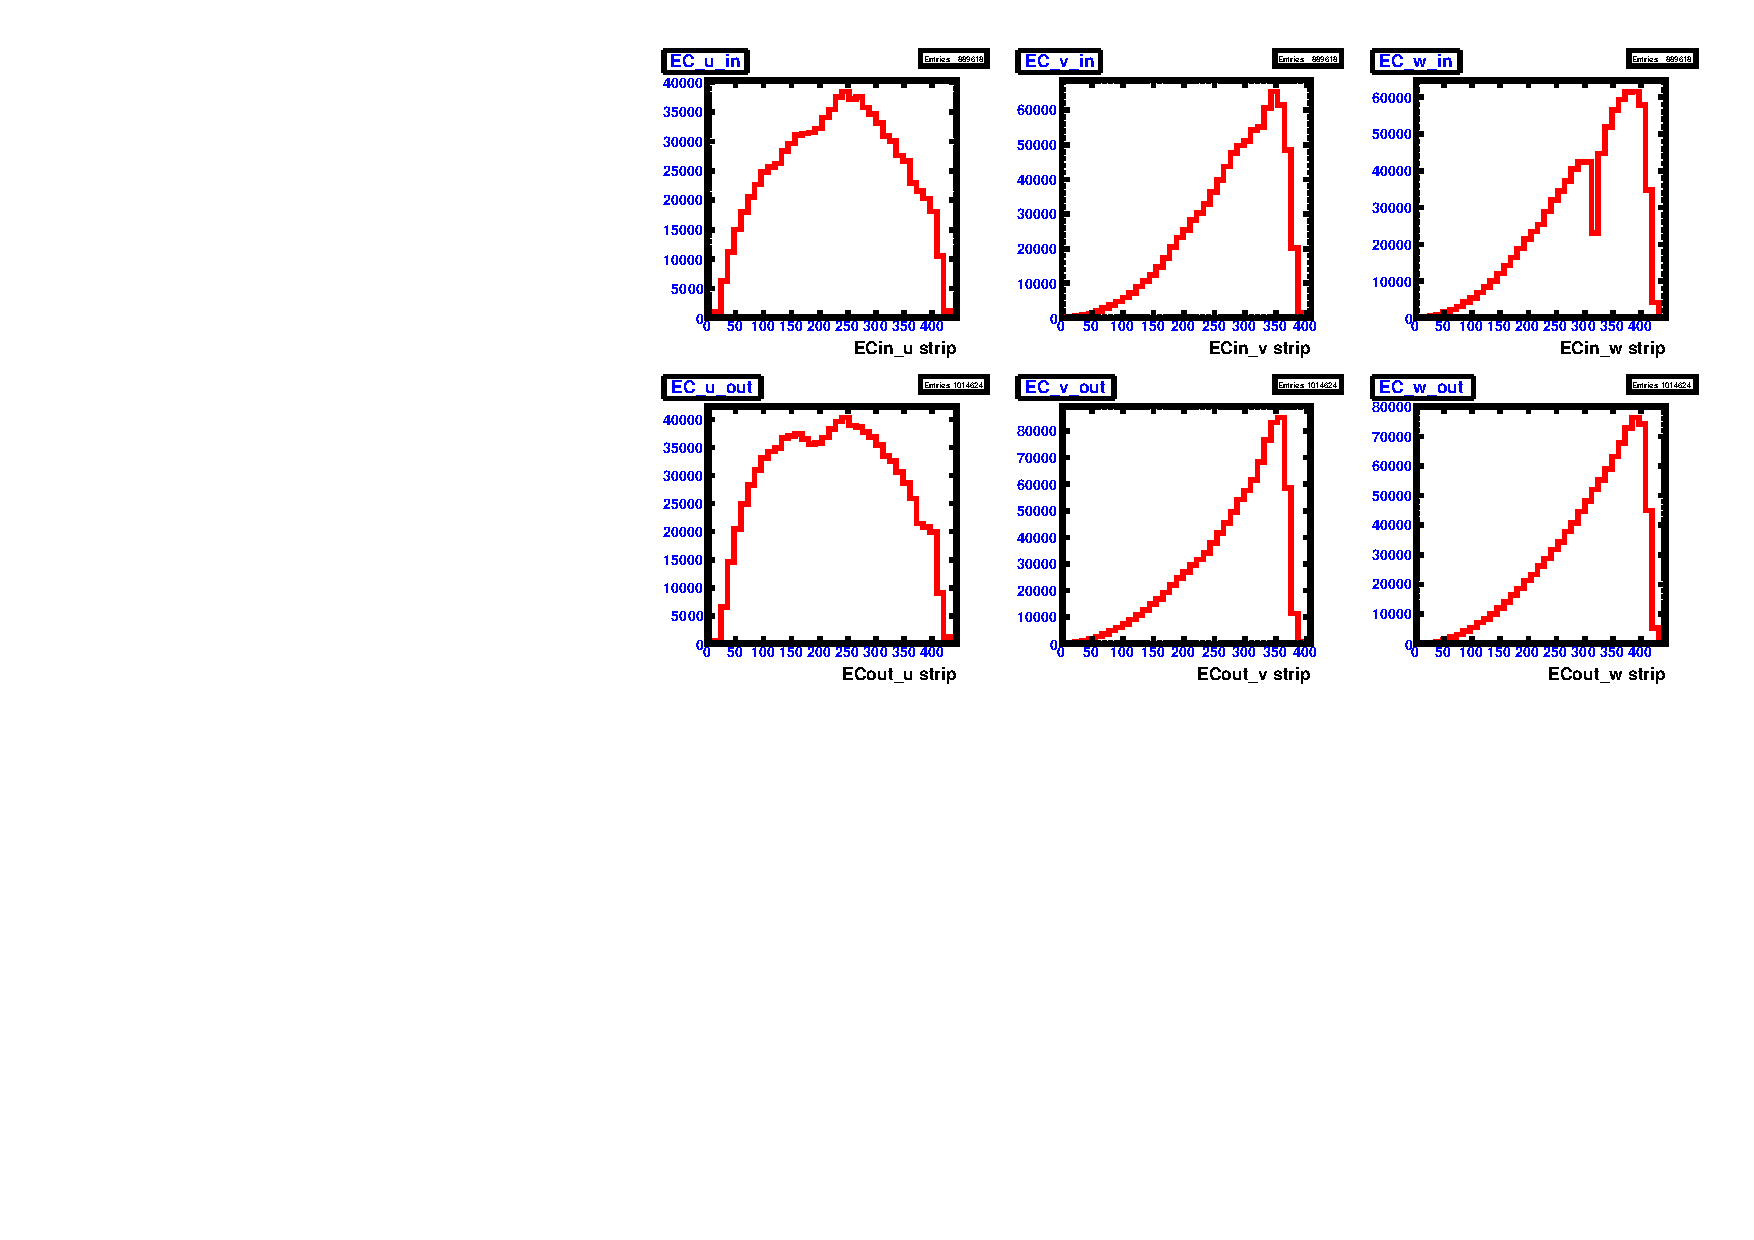
\includegraphics[width=\figwidth, height=3.5in,valign=c]{\grpath/analysis/FIDUCIAL_CUTS/EC/pim_ecuvw_NOKnockout_sec1.pdf}\label{fig:EC_II_I}} \\

      \caption {Inefficient \abbr{EC} $u$, $v$, $w$ strips vs. $\phi$ for sector 1 in \abbr{CLAS} $e^{-} \ $ data~(\ref{fig:EC_I_I}), notation the same as Fig.~\ref{fig:neg:ec.sec5}. Number of hits vs. inefficient \abbr{EC} $u$, $v$, $w$ strips for sector 1 for $e^-$ data~(\ref{fig:EC_II_I}). Notation same as in Fig.~\ref{fig:neg.ecstrip.sec5}.}
        \label{fig:EC_no_I}
\end{figure}



\begin{figure}[!ht]
  \centering
  \subfloat[][]{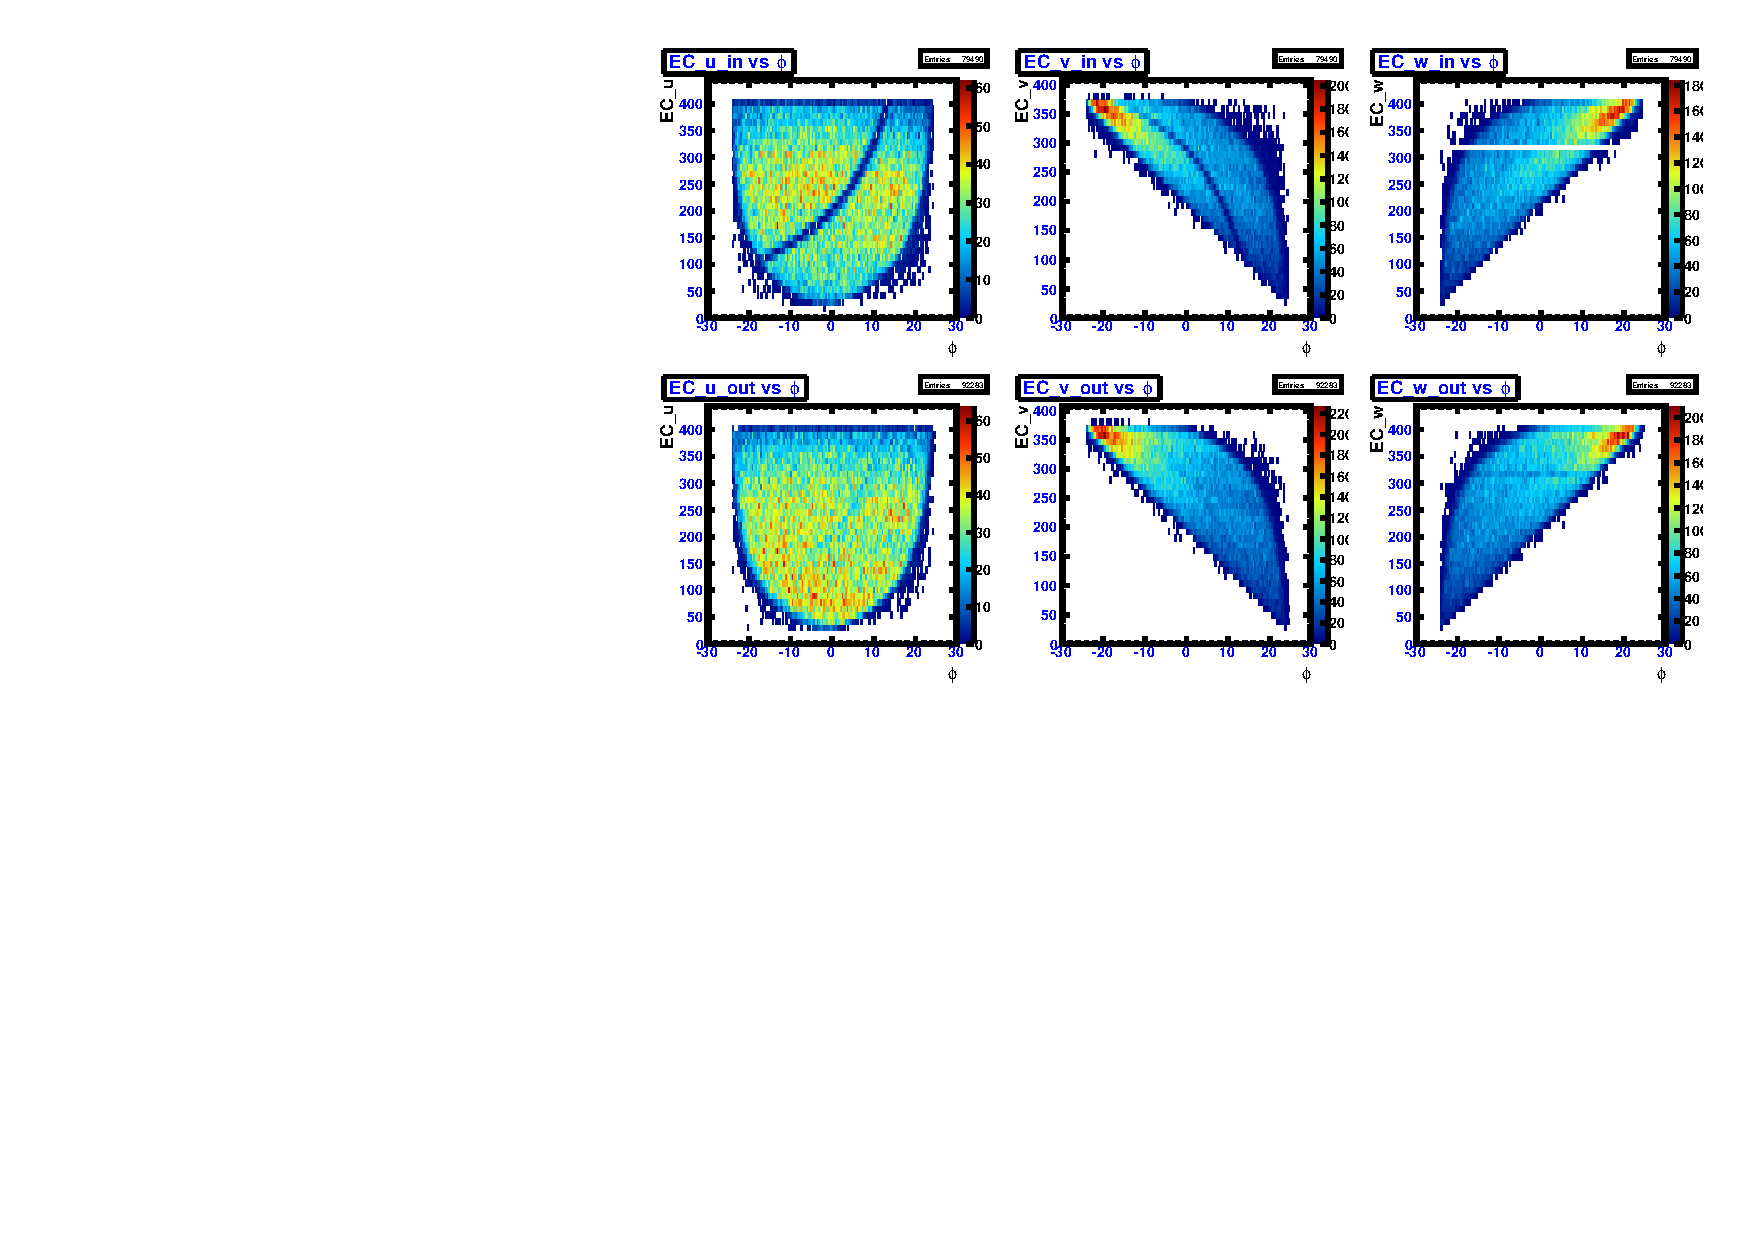
\includegraphics[width=\figwidth, height=3.5in,valign=c]{\grpath/analysis/FIDUCIAL_CUTS/EC/pim_ecuvw_phi_afterGeoFid_sec1.pdf}\label{fig:EC_III_I}} \quad
  \\
  \subfloat[][]{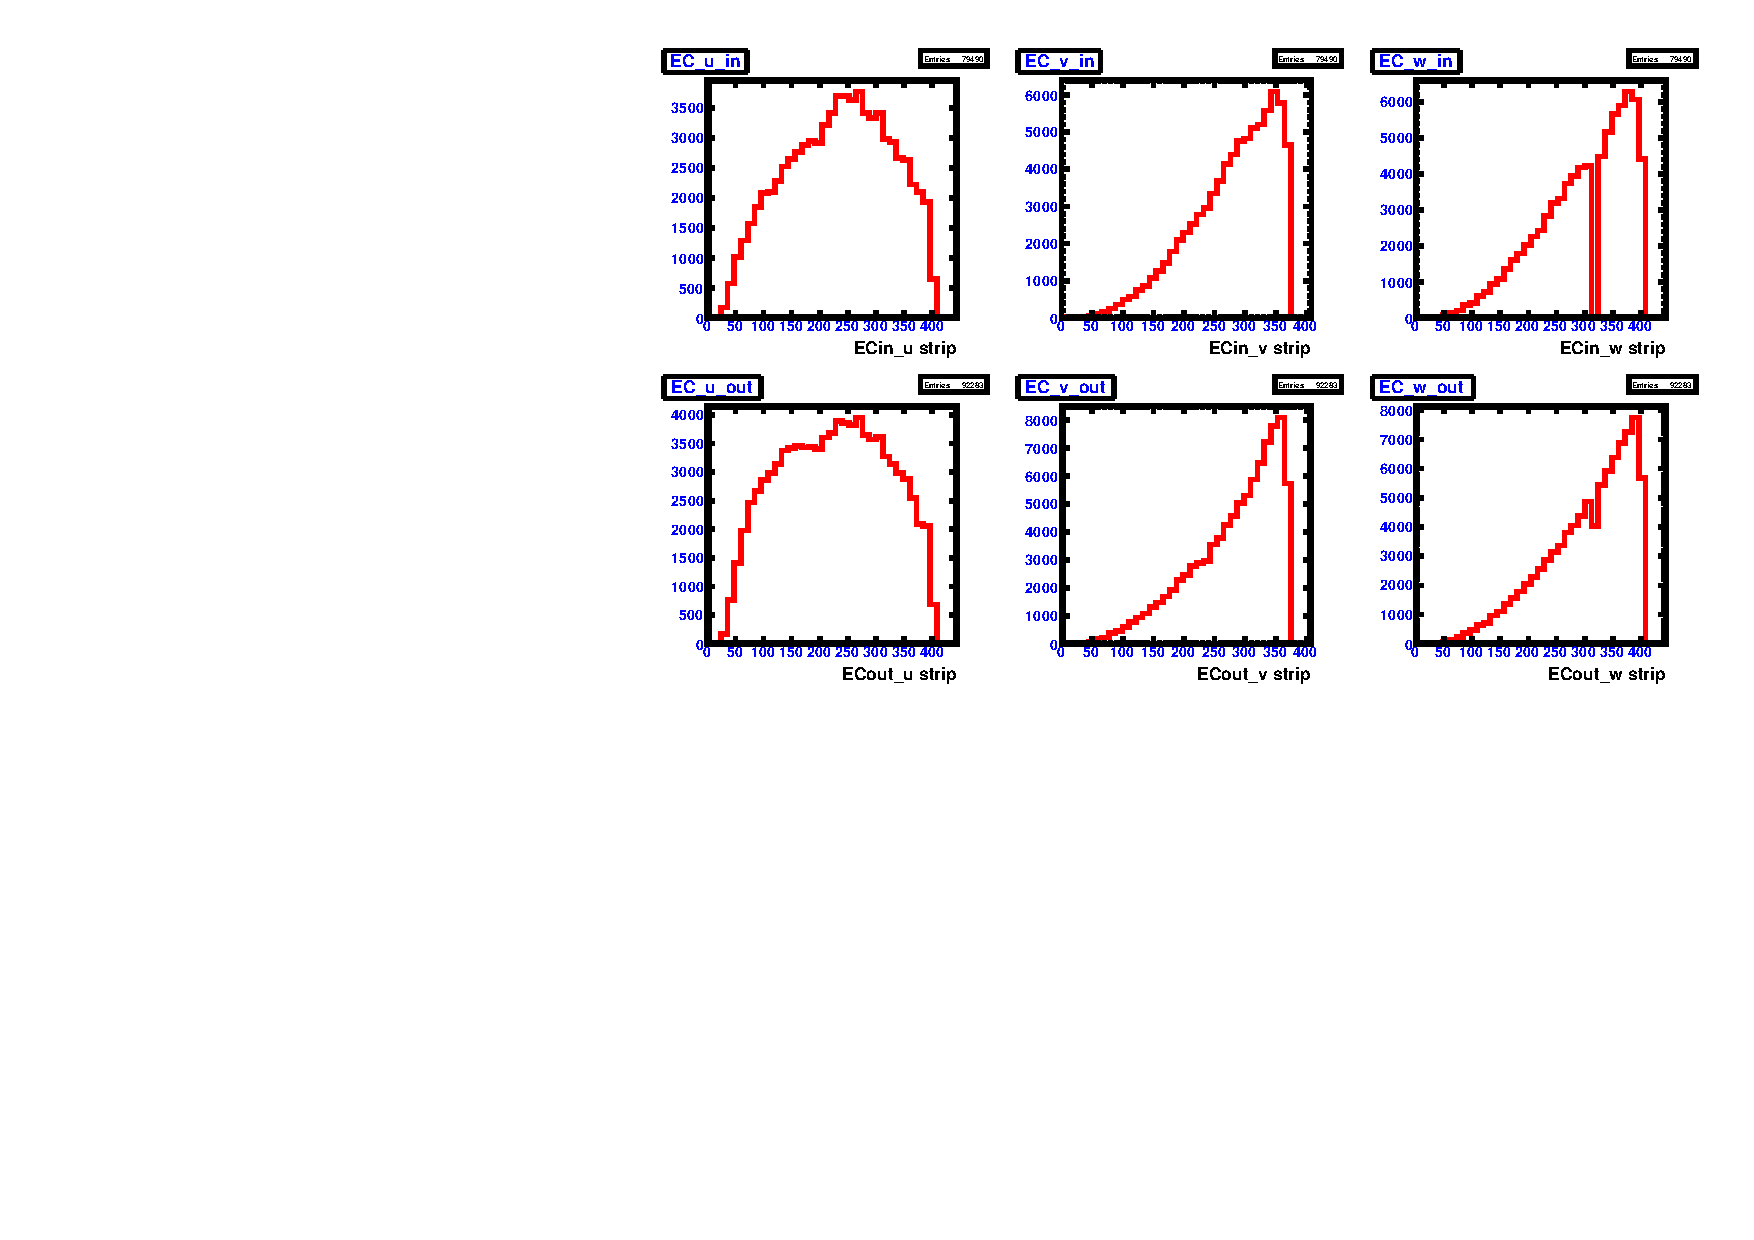
\includegraphics[width=\figwidth, height=3.5in,valign=c]{\grpath/analysis/FIDUCIAL_CUTS/EC/pim_ecuvw_afterGeoFid_sec1.pdf}\label{fig:EC_IV_I}} \\

      \caption {\abbr{EC} $u$, $v$, $w$ strips vs. $\phi$ for sector 1 with fiducial cuts and inefficient paddle knockouts applied to $e^-$ data~(\ref{fig:EC_III_I}), notation the same as Fig.~\ref{fig:neg:ec.sec5_cut}. Number of hits vs. \abbr{EC} $u$, $v$, $w$ strips for sector 1 with fiducial cuts and inefficient paddle knockouts applied to $e^-$ data~(\ref{fig:EC_IV_I}). Notation same as in Fig.~\ref{fig:neg.ecstrip.sec5_cut}.}
        \label{fig:EC_cut_I}
\end{figure}


% % % %SECTOR 2
\begin{figure}[!ht]
  \centering
  \subfloat[][]{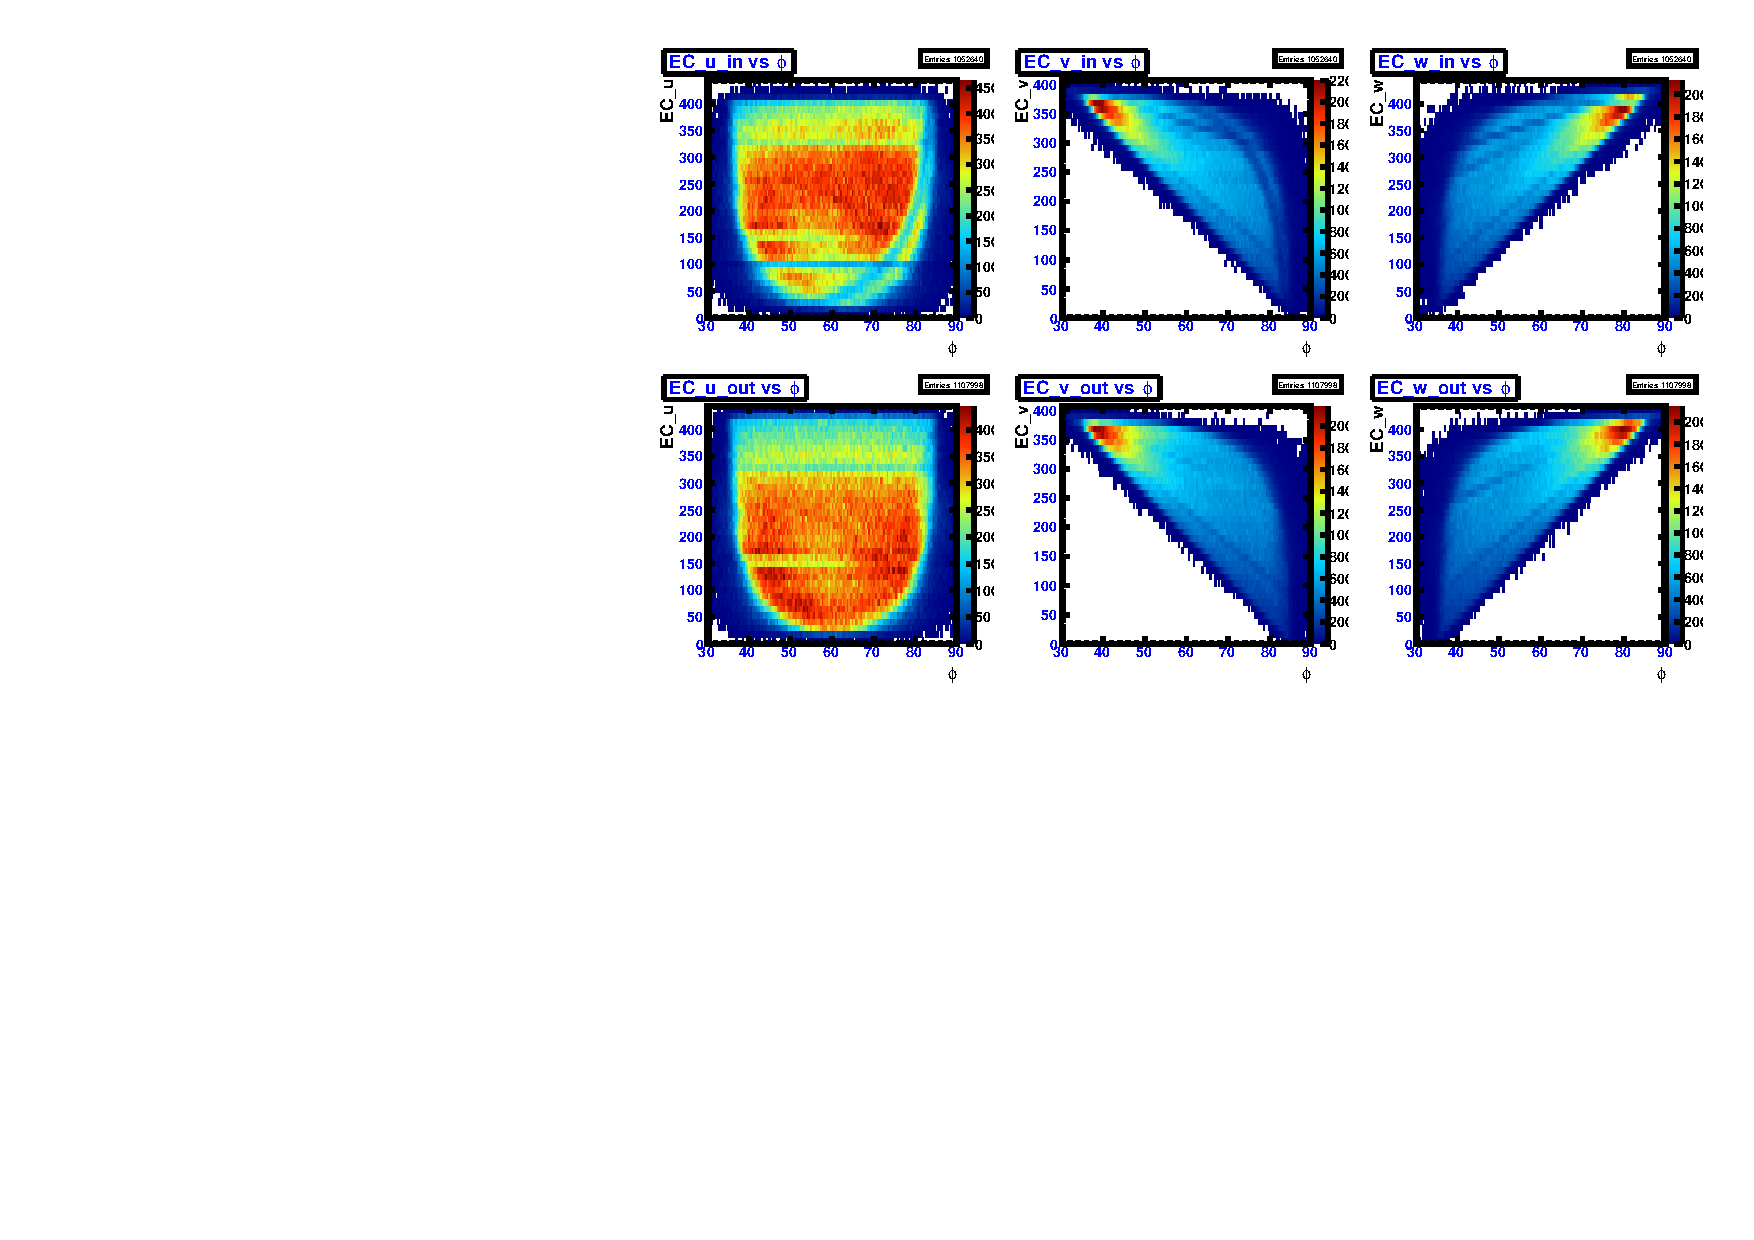
\includegraphics[width=\figwidth, height=3.5in,valign=c]{\grpath/analysis/FIDUCIAL_CUTS/EC/pim_ecuvw_phi_NOKnockout_sec2.pdf}\label{fig:EC_I_II}} \quad
  \\
  \subfloat[][]{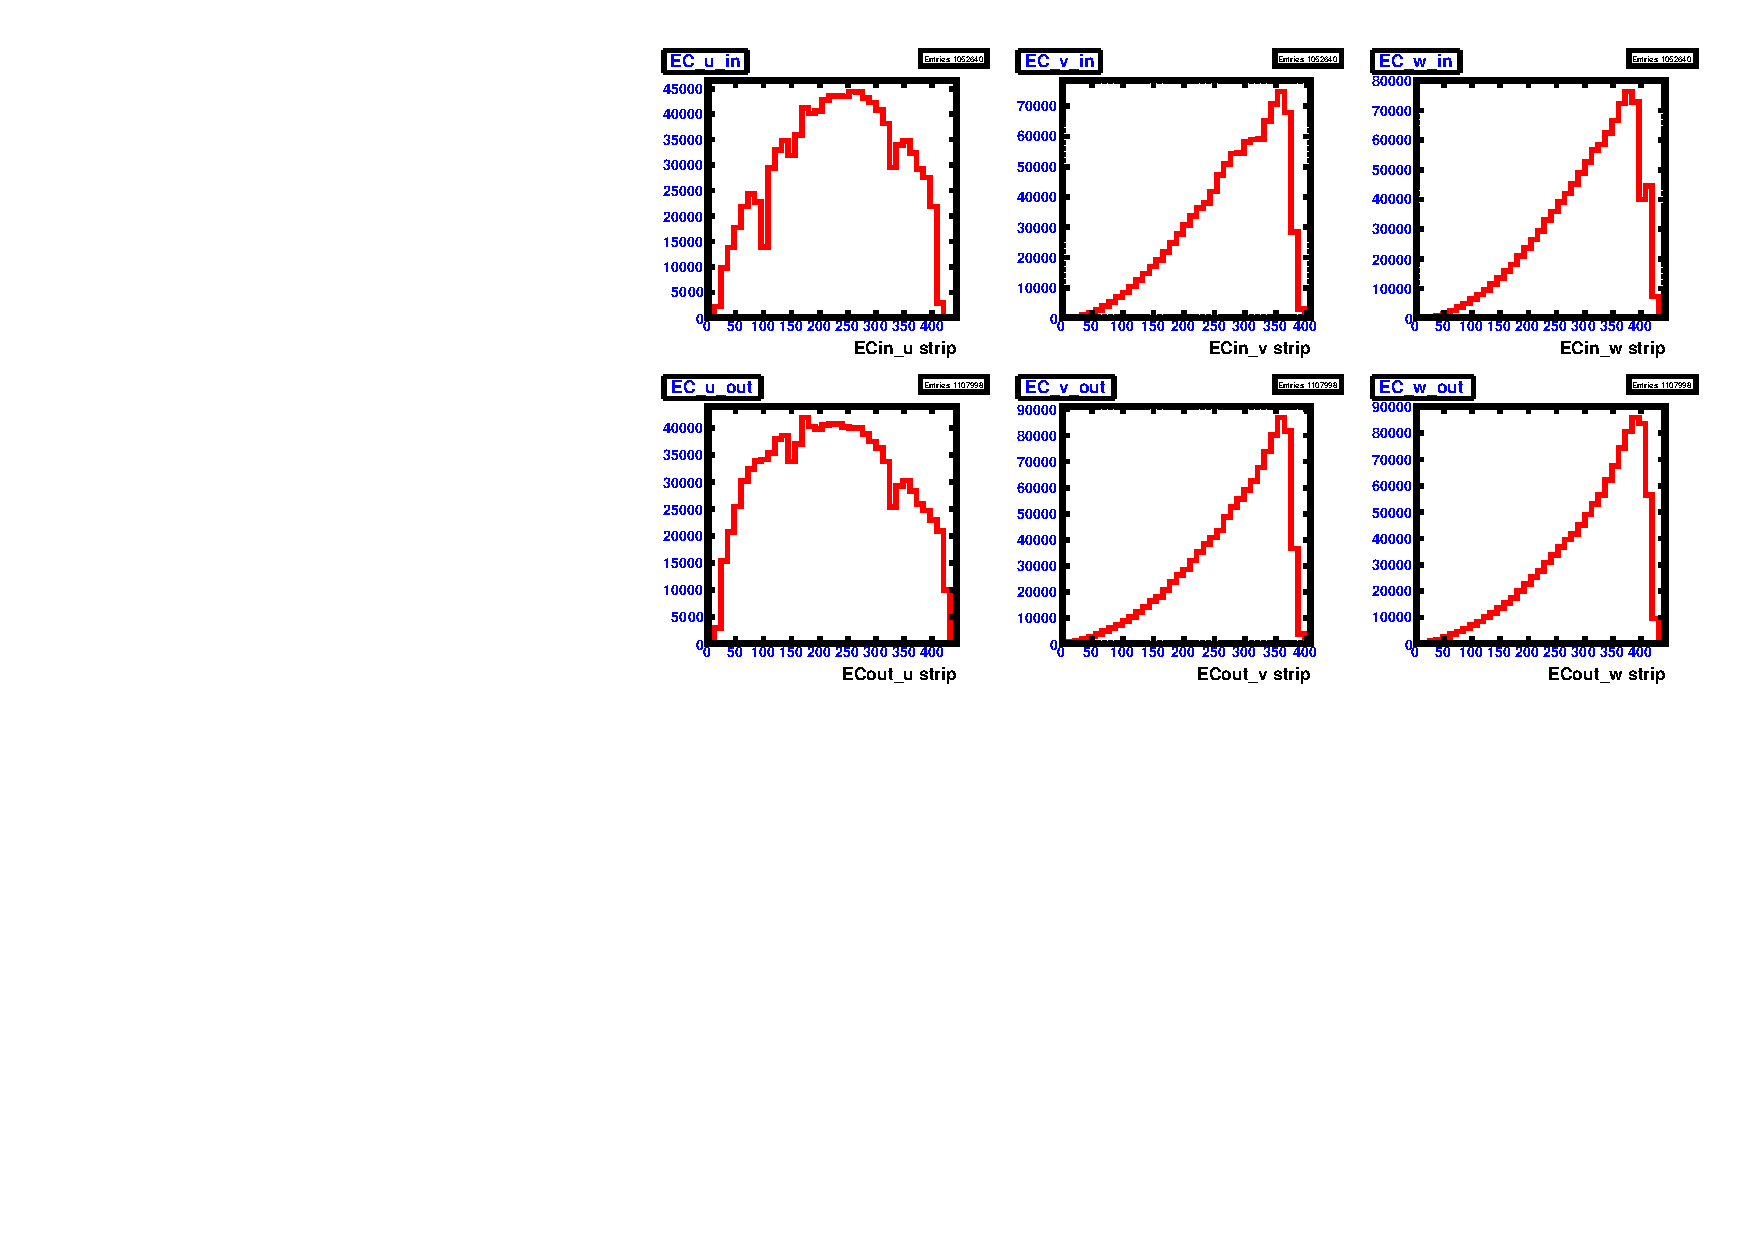
\includegraphics[width=\figwidth, height=3.5in,valign=c]{\grpath/analysis/FIDUCIAL_CUTS/EC/pim_ecuvw_NOKnockout_sec2.pdf}\label{fig:EC_II_II}} \\

      \caption {Inefficient \abbr{EC} $u$, $v$, $w$ strips vs. $\phi$ for sector 2 in \abbr{CLAS} $e^{-} \ $ data~(\ref{fig:EC_I_II}), notation the same as Fig.~\ref{fig:neg:ec.sec5}. Number of hits vs. inefficient \abbr{EC} $u$, $v$, $w$ strips for sector 2 for $e^-$ data~(\ref{fig:EC_II_II}). Notation same as in Fig.~\ref{fig:neg.ecstrip.sec5}.}
        \label{fig:EC_no_II}
\end{figure}



\begin{figure}[!ht]
  \centering
  \subfloat[][]{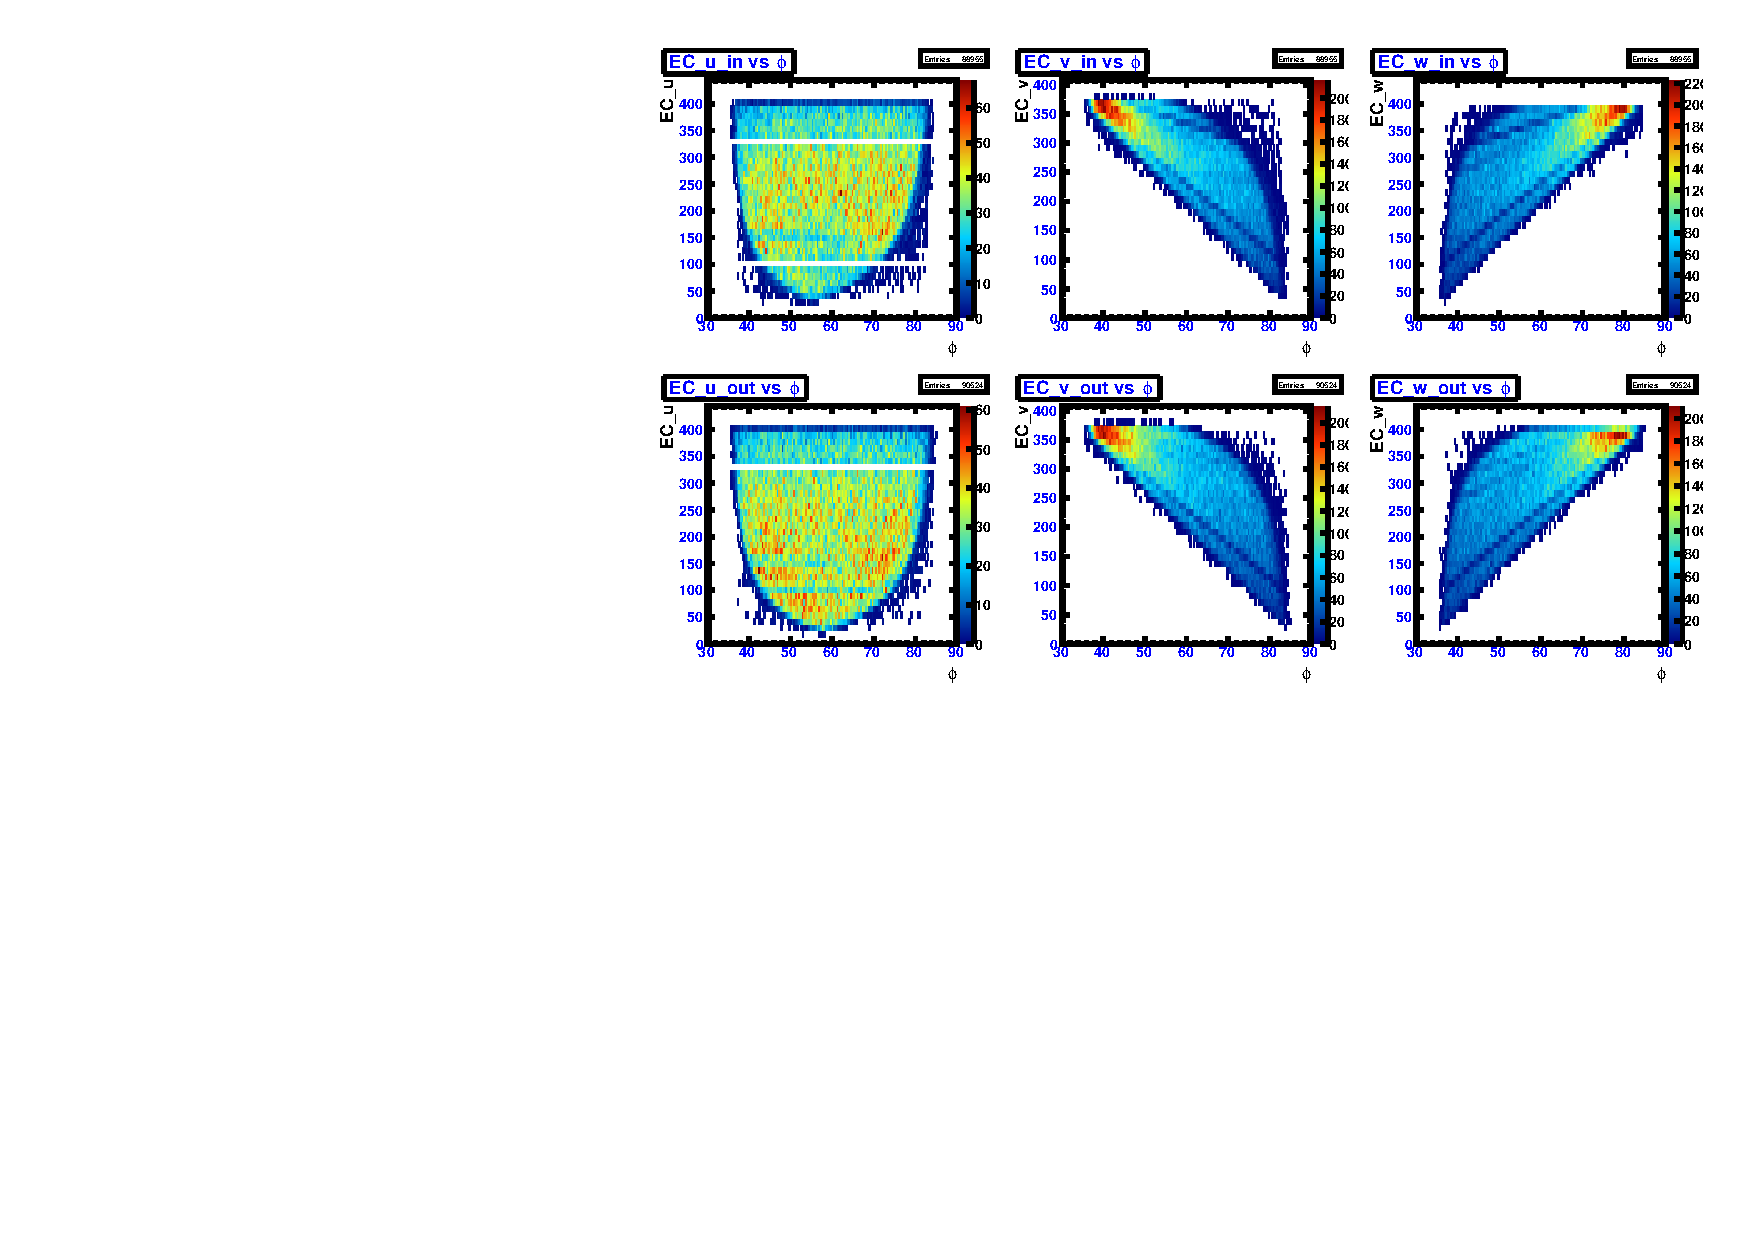
\includegraphics[width=\figwidth, height=3.5in,valign=c]{\grpath/analysis/FIDUCIAL_CUTS/EC/pim_ecuvw_phi_afterGeoFid_sec2.pdf}\label{fig:EC_III_II}} \quad
  \\
  \subfloat[][]{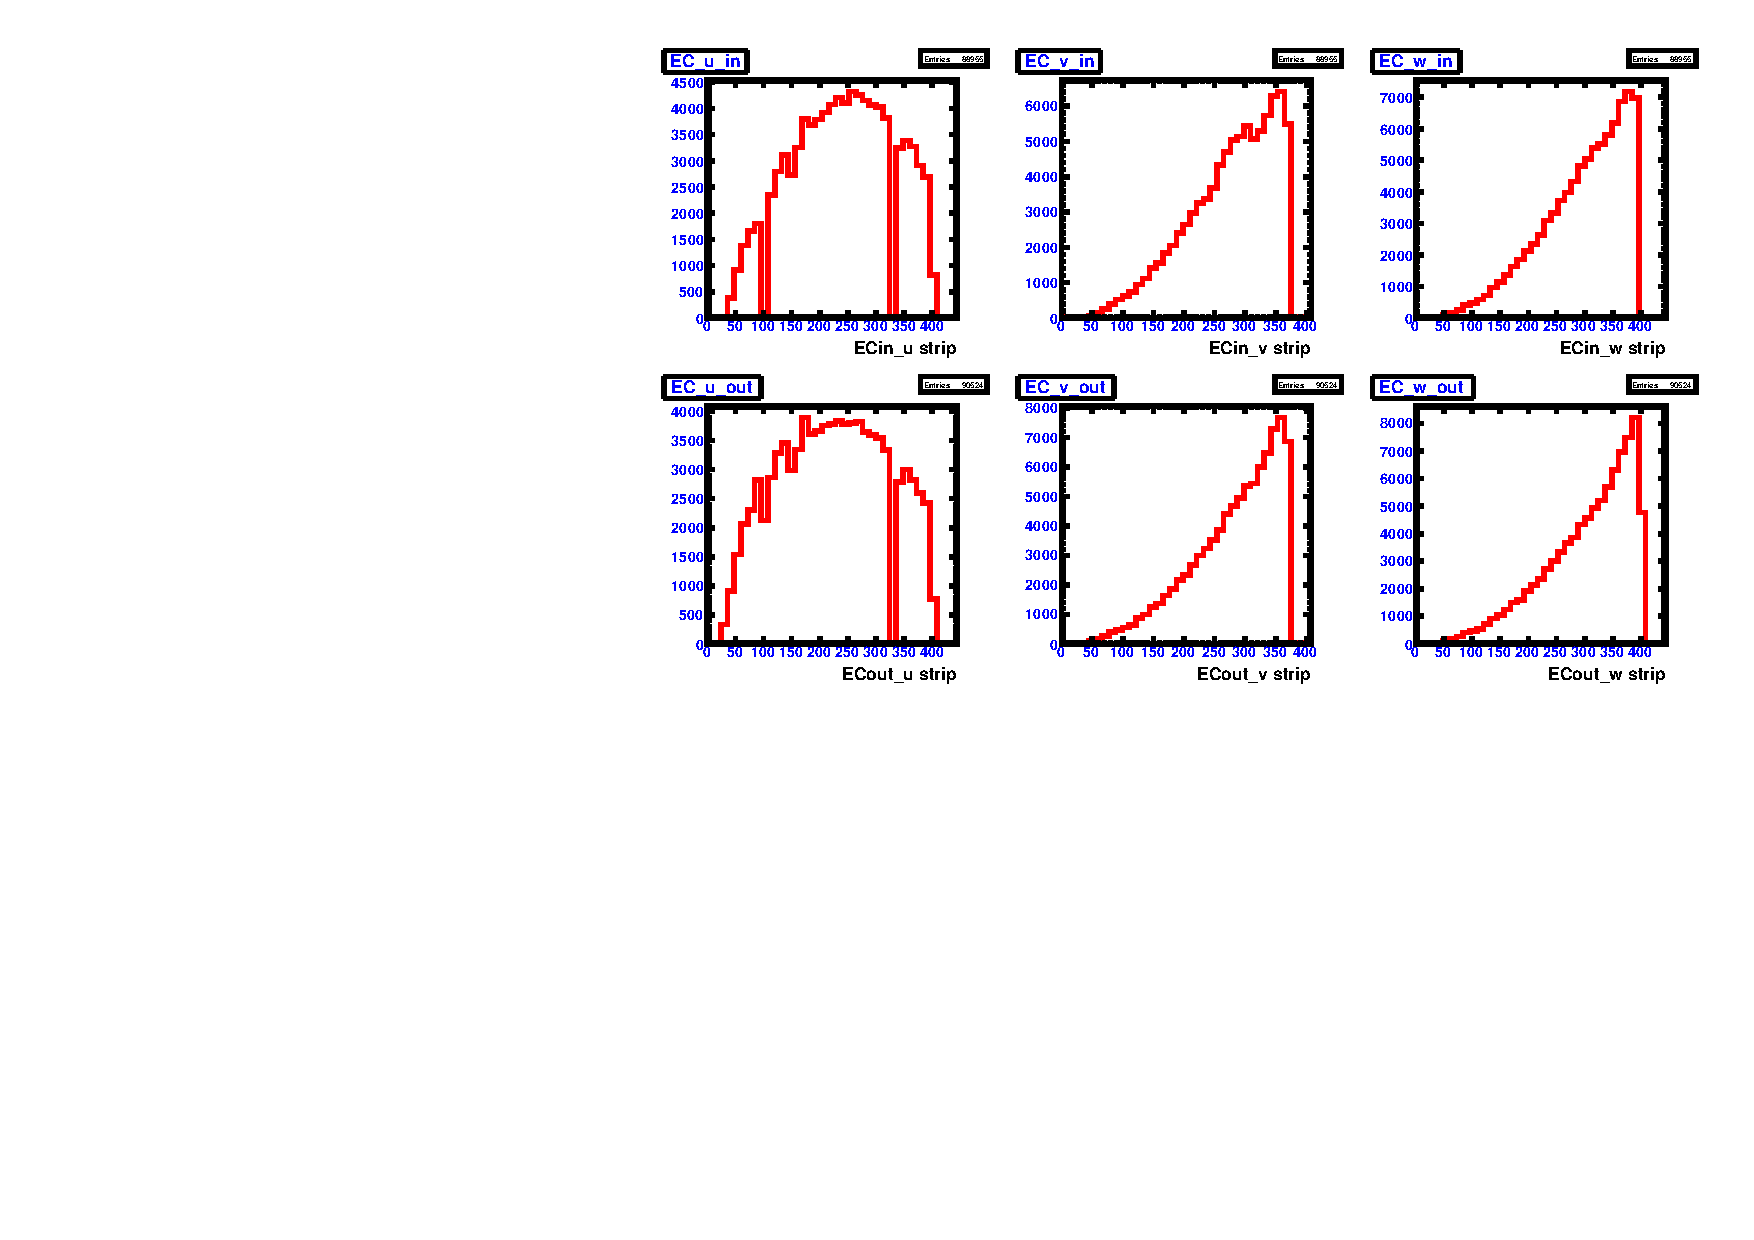
\includegraphics[width=\figwidth, height=3.5in,valign=c]{\grpath/analysis/FIDUCIAL_CUTS/EC/pim_ecuvw_afterGeoFid_sec2.pdf}\label{fig:EC_IV_II}} \\

      \caption {\abbr{EC} $u$, $v$, $w$ strips vs. $\phi$ for sector 2 with fiducial cuts and inefficient paddle knockouts applied to $e^-$ data~(\ref{fig:EC_III_II}), notation the same as Fig.~\ref{fig:neg:ec.sec5_cut}. Number of hits vs. \abbr{EC} $u$, $v$, $w$ strips for sector 2 with fiducial cuts and inefficient paddle knockouts applied to $e^-$ data~(\ref{fig:EC_IV_II}). Notation same as in Fig.~\ref{fig:neg.ecstrip.sec5_cut}.}
        \label{fig:EC_cut_II}
\end{figure}


% % % %SECTOR 3
\begin{figure}[!ht]
  \centering
  \subfloat[][]{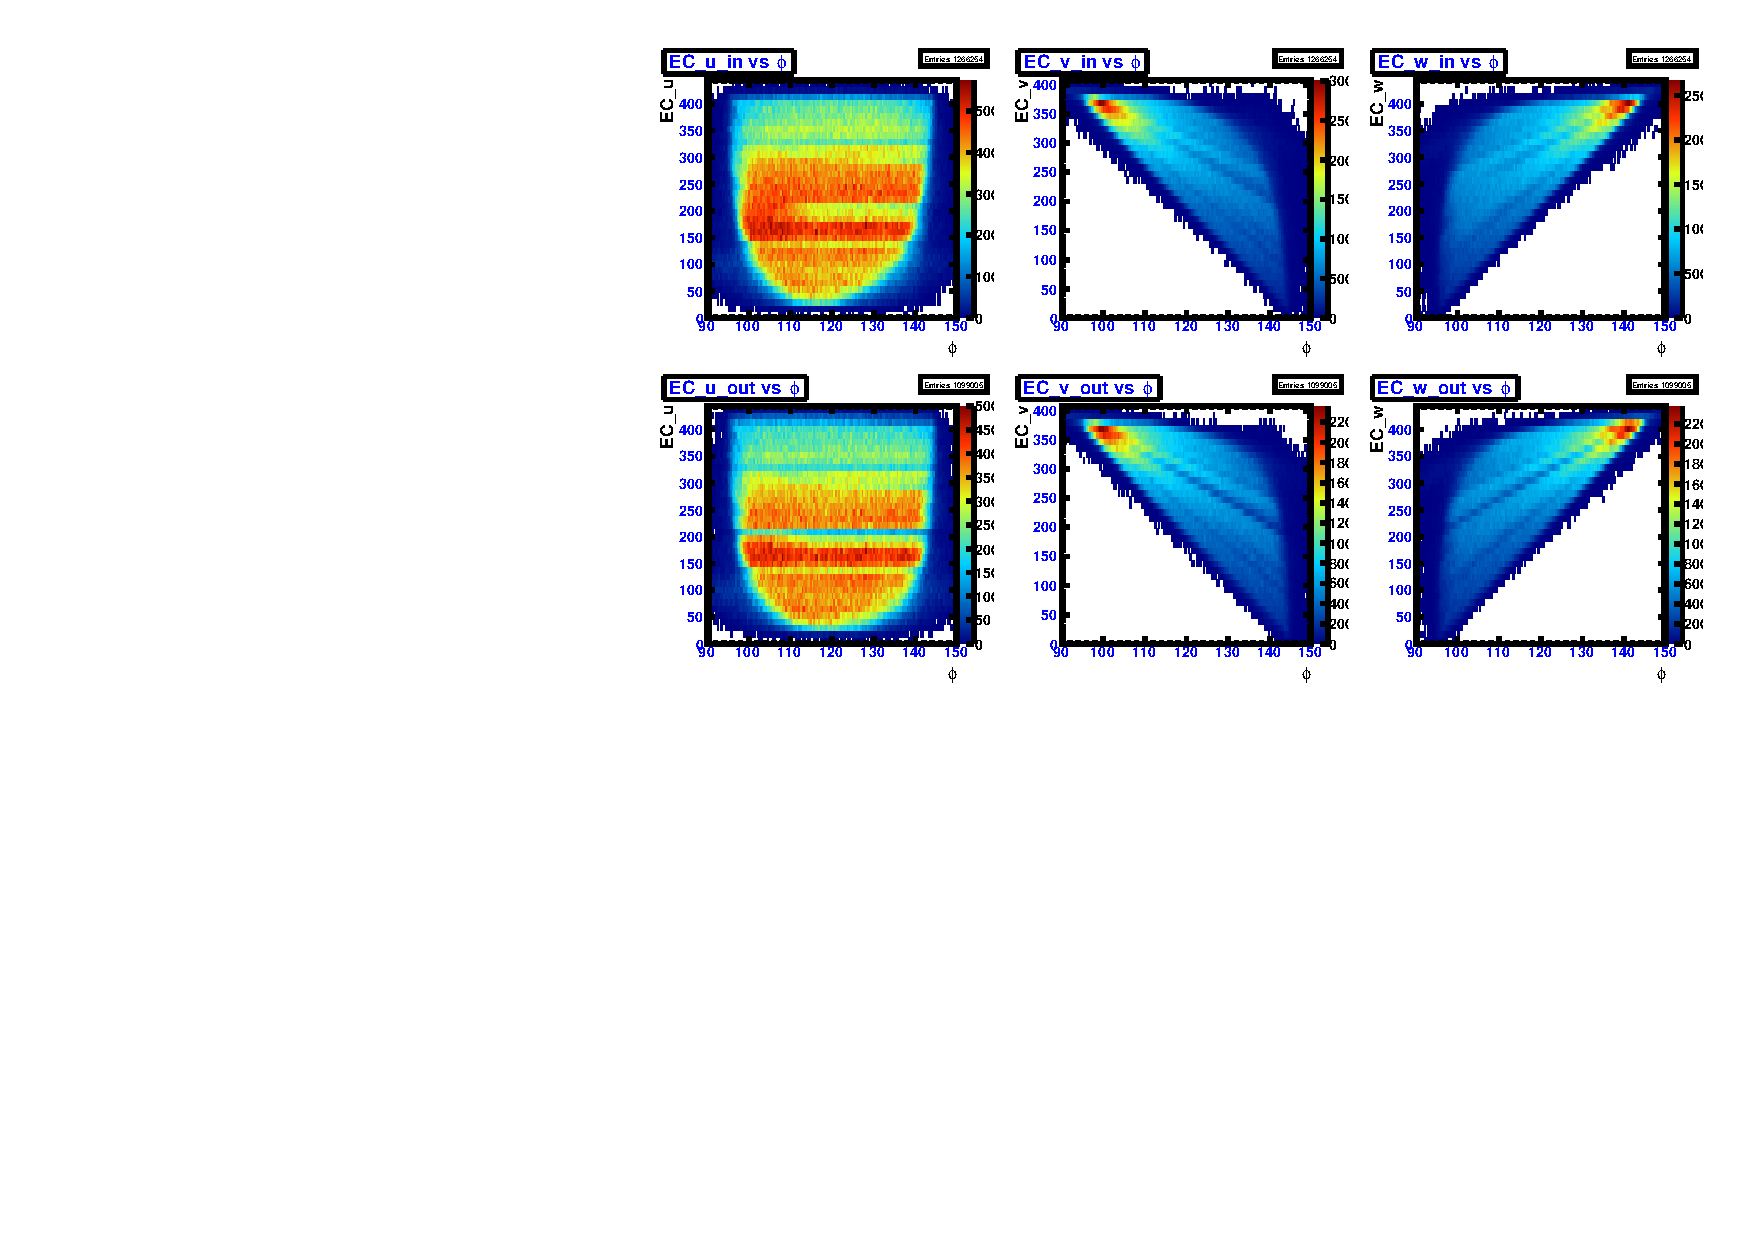
\includegraphics[width=\figwidth, height=3.5in,valign=c]{\grpath/analysis/FIDUCIAL_CUTS/EC/pim_ecuvw_phi_NOKnockout_sec3.pdf}\label{fig:EC_I_III}} \quad
  \\
  \subfloat[][]{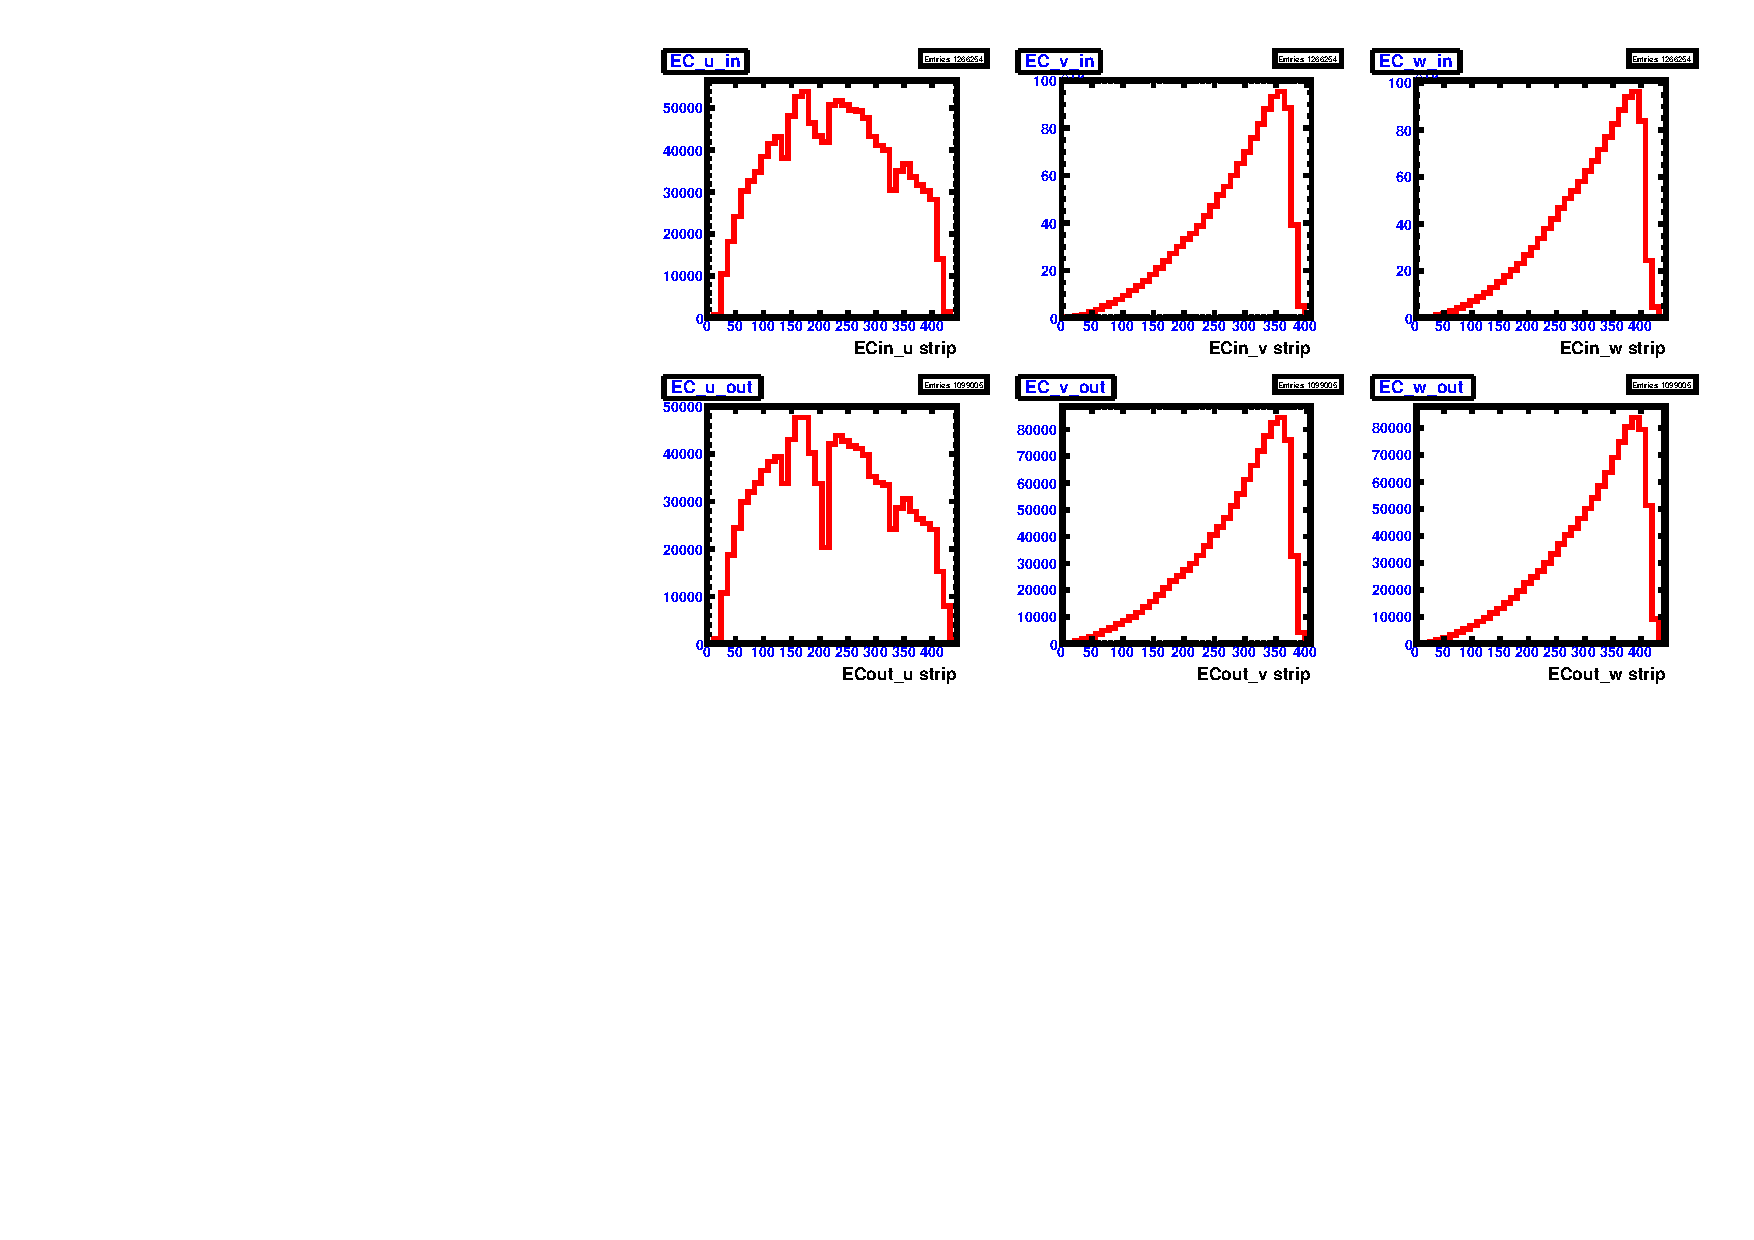
\includegraphics[width=\figwidth, height=3.5in,valign=c]{\grpath/analysis/FIDUCIAL_CUTS/EC/pim_ecuvw_NOKnockout_sec3.pdf}\label{fig:EC_II_III}} \\

      \caption {Inefficient \abbr{EC} $u$, $v$, $w$ strips vs. $\phi$ for sector 3 in \abbr{CLAS} $e^{-} \ $ data~(\ref{fig:EC_I_III}), notation the same as Fig.~\ref{fig:neg:ec.sec5}. Number of hits vs. inefficient \abbr{EC} $u$, $v$, $w$ strips for sector 3 for $e^-$ data~(\ref{fig:EC_II_III}). Notation same as in Fig.~\ref{fig:neg.ecstrip.sec5}.}
        \label{fig:EC_no_III}
\end{figure}



\begin{figure}[!ht]
  \centering
  \subfloat[][]{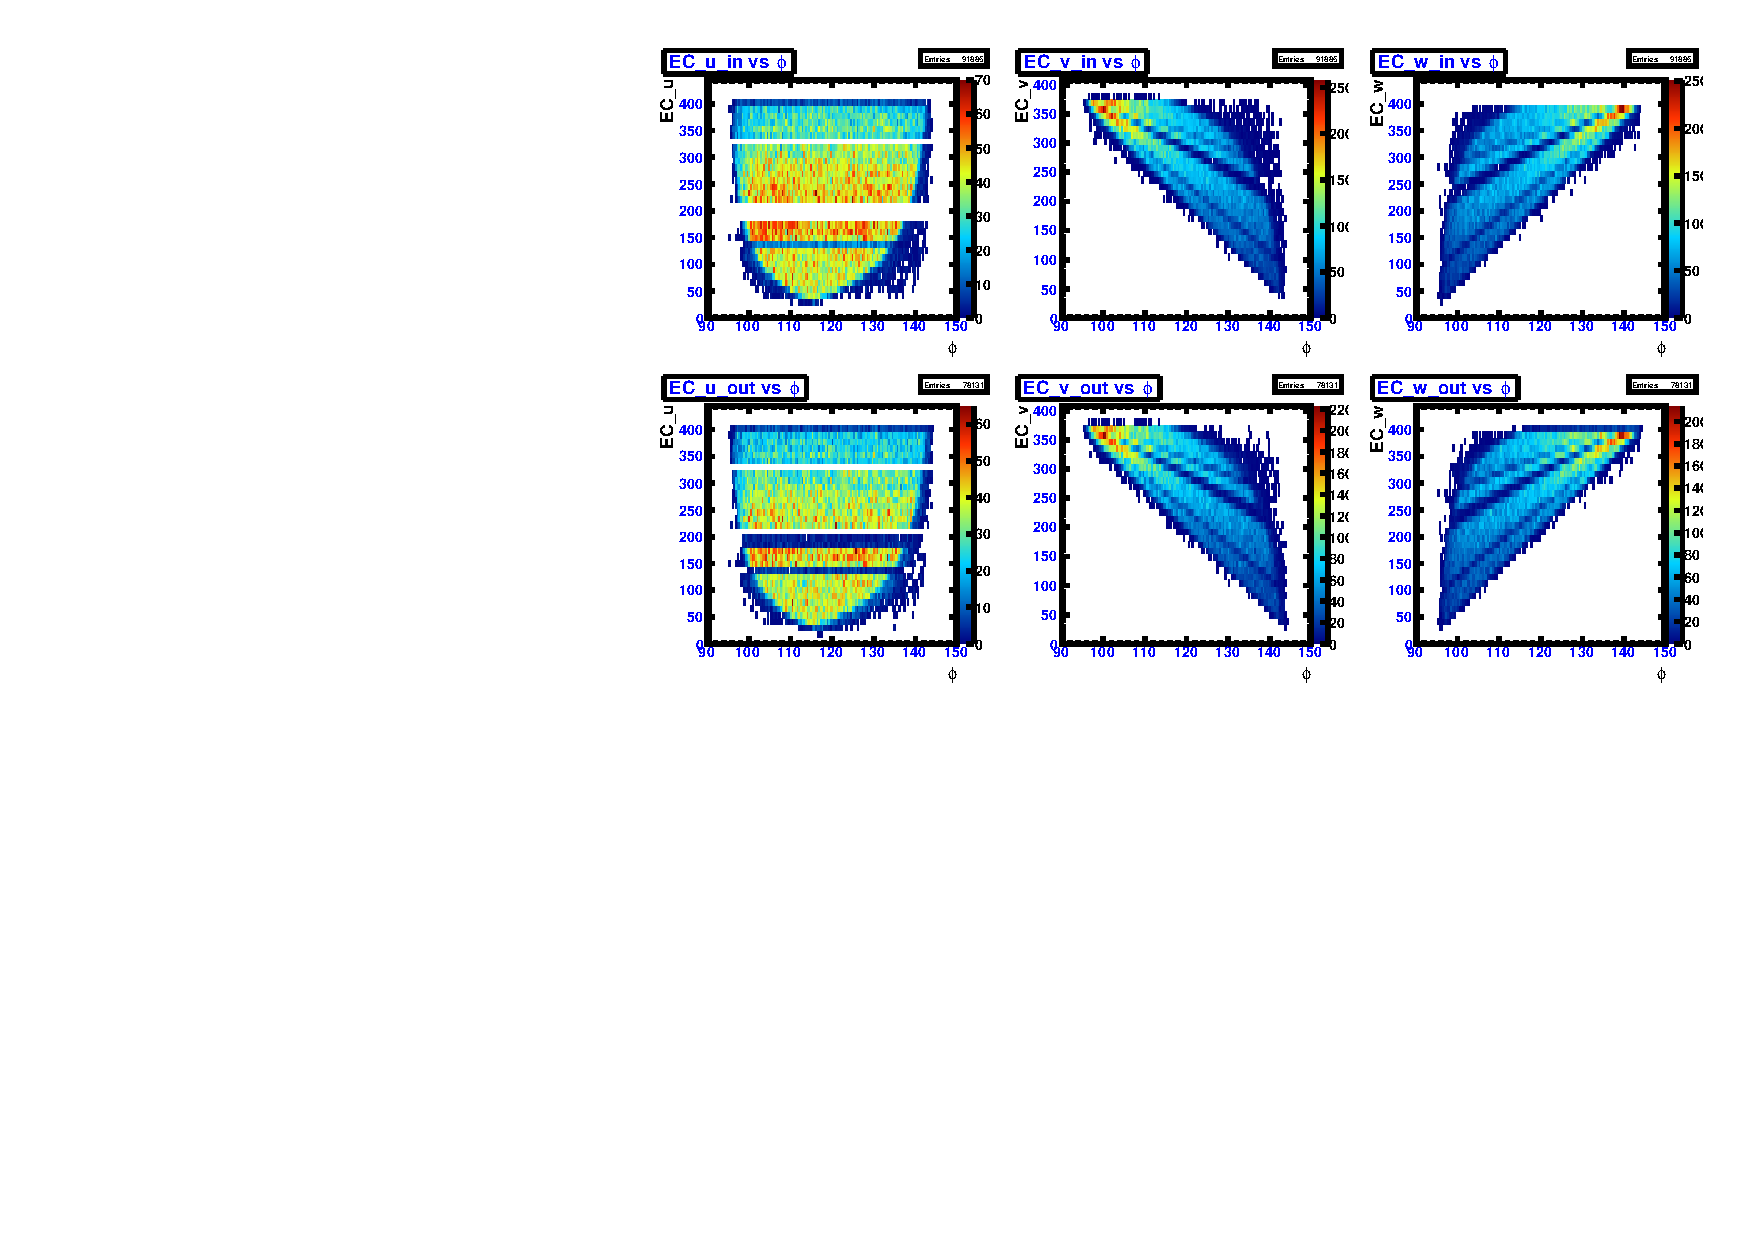
\includegraphics[width=\figwidth, height=3.5in,valign=c]{\grpath/analysis/FIDUCIAL_CUTS/EC/pim_ecuvw_phi_afterGeoFid_sec3.pdf}\label{fig:EC_III_III}} \quad
  \\
  \subfloat[][]{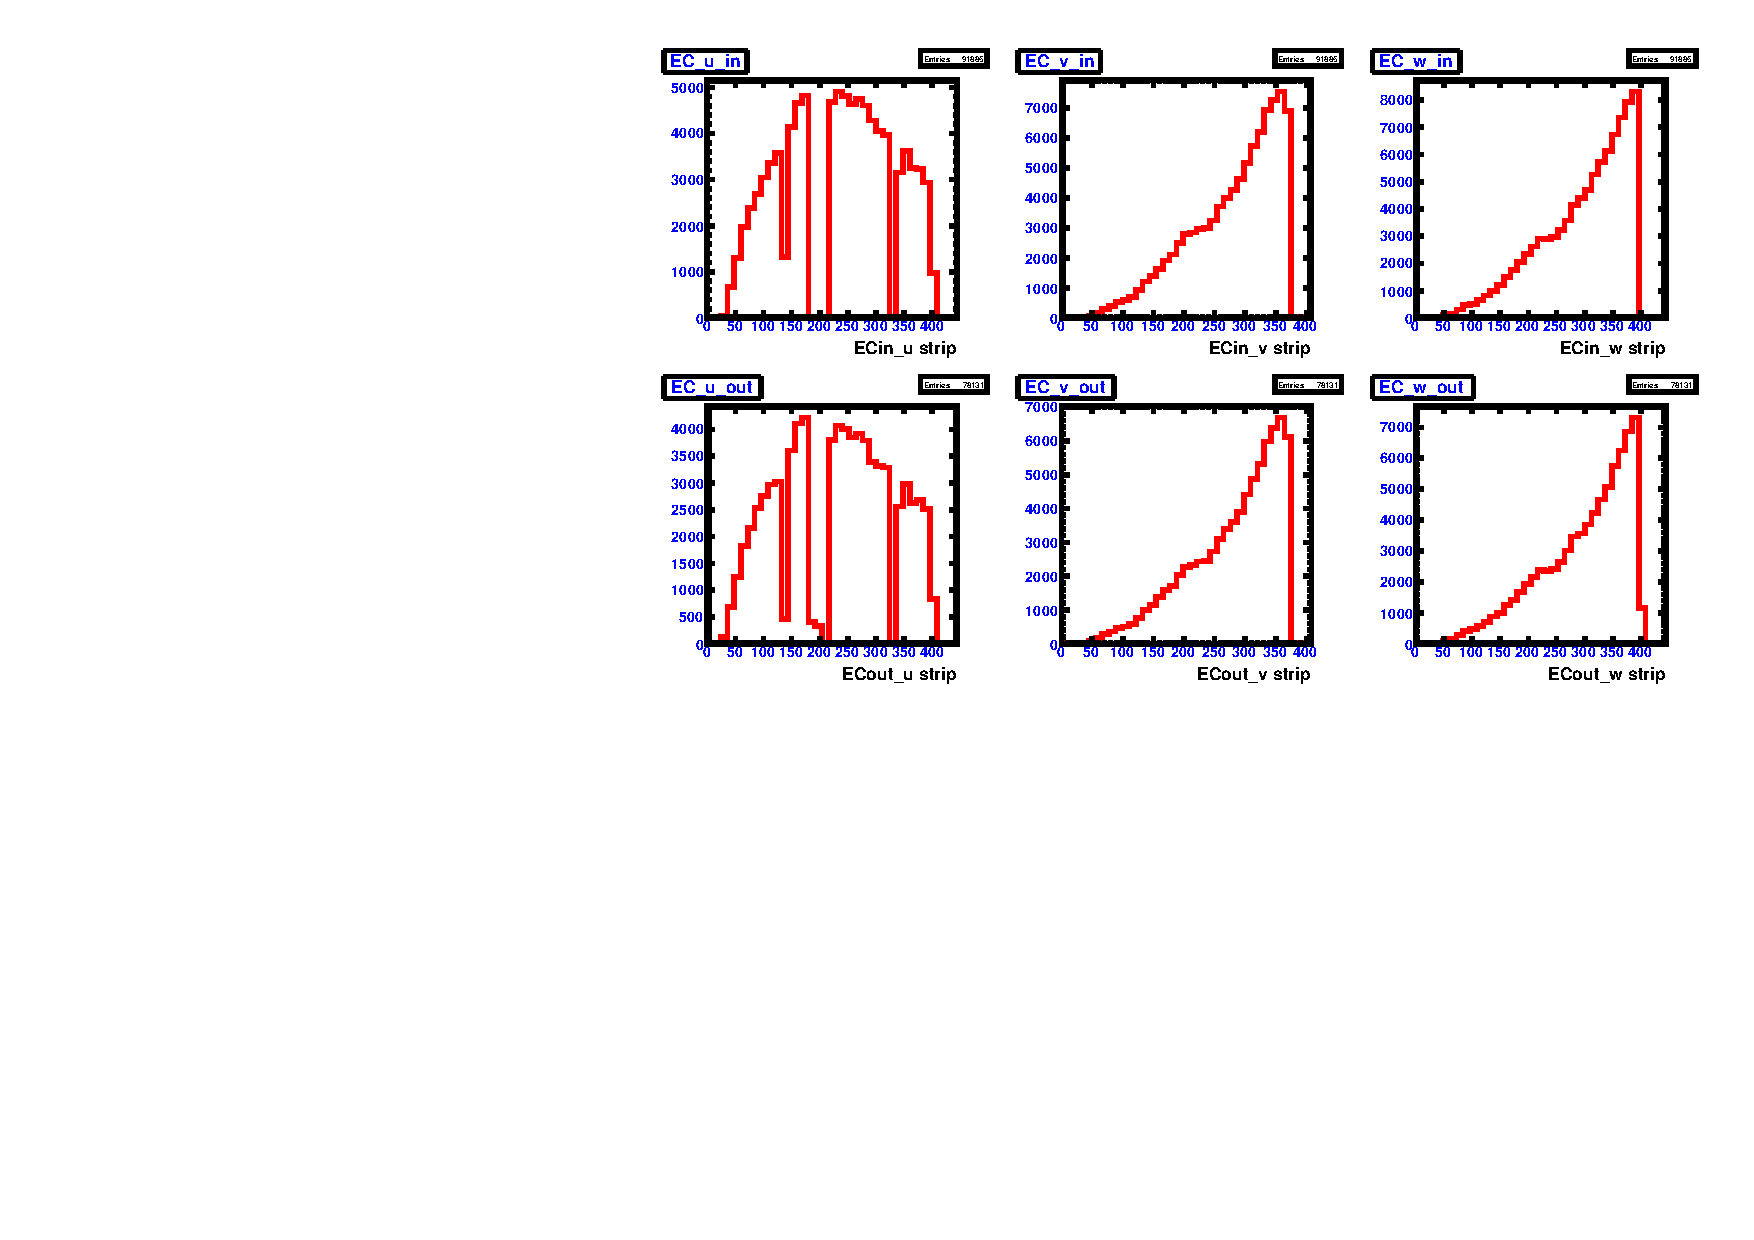
\includegraphics[width=\figwidth, height=3.5in,valign=c]{\grpath/analysis/FIDUCIAL_CUTS/EC/pim_ecuvw_afterGeoFid_sec3.pdf}\label{fig:EC_IV_III}} \\

      \caption {\abbr{EC} $u$, $v$, $w$ strips vs. $\phi$ for sector 3 with fiducial cuts and inefficient paddle knockouts applied to $e^-$ data~(\ref{fig:EC_III_III}), notation the same as Fig.~\ref{fig:neg:ec.sec5_cut}. Number of hits vs. \abbr{EC} $u$, $v$, $w$ strips for sector 3 with fiducial cuts and inefficient paddle knockouts applied to $e^-$ data~(\ref{fig:EC_IV_III}). Notation same as in Fig.~\ref{fig:neg.ecstrip.sec5_cut}.}
        \label{fig:EC_cut_III}
\end{figure}


% % % %SECTOR 4
\begin{figure}[!ht]
  \centering
  \subfloat[][]{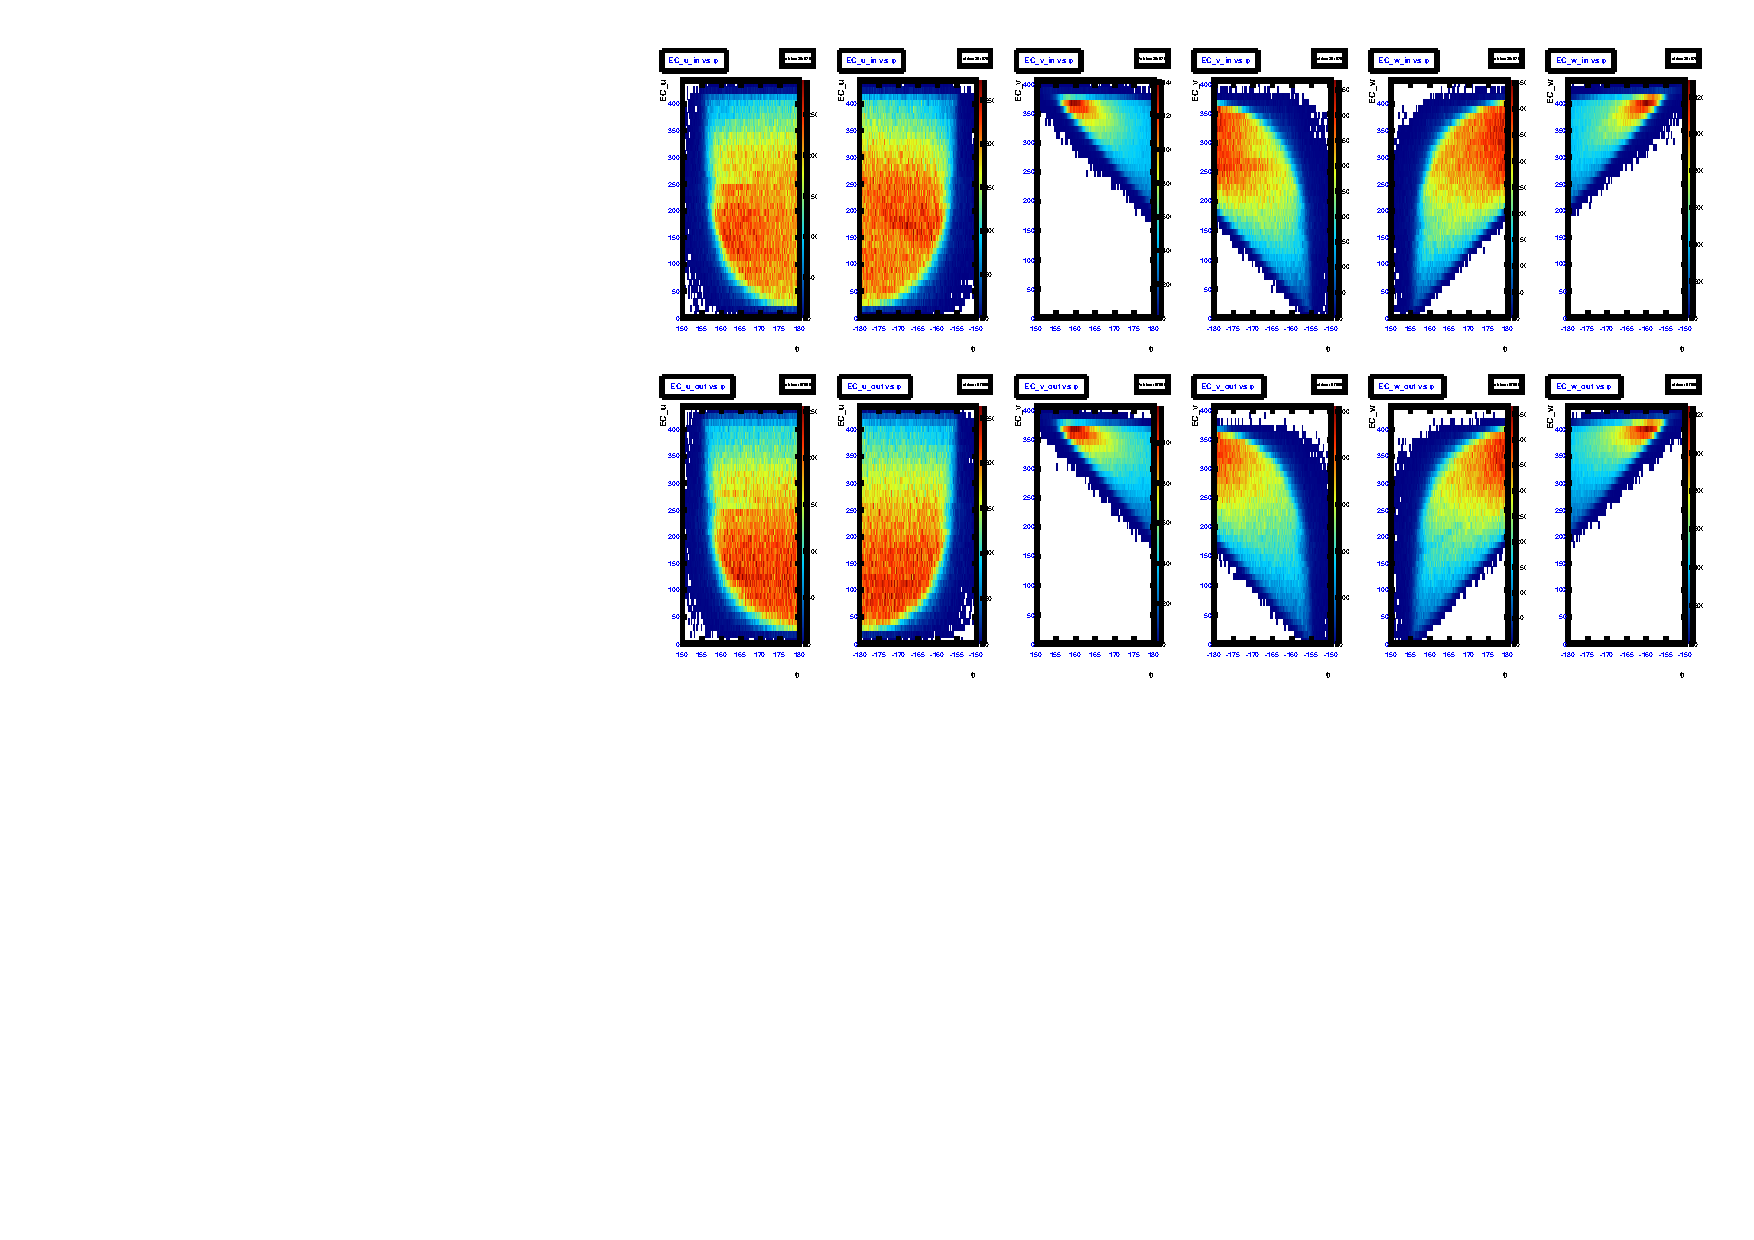
\includegraphics[width=\figwidth, height=3.5in,valign=c]{\grpath/analysis/FIDUCIAL_CUTS/EC/pim_ecuvw_phi_NOKnockout_sec4.pdf}\label{fig:EC_I_IV}} \quad
  \\
  \subfloat[][]{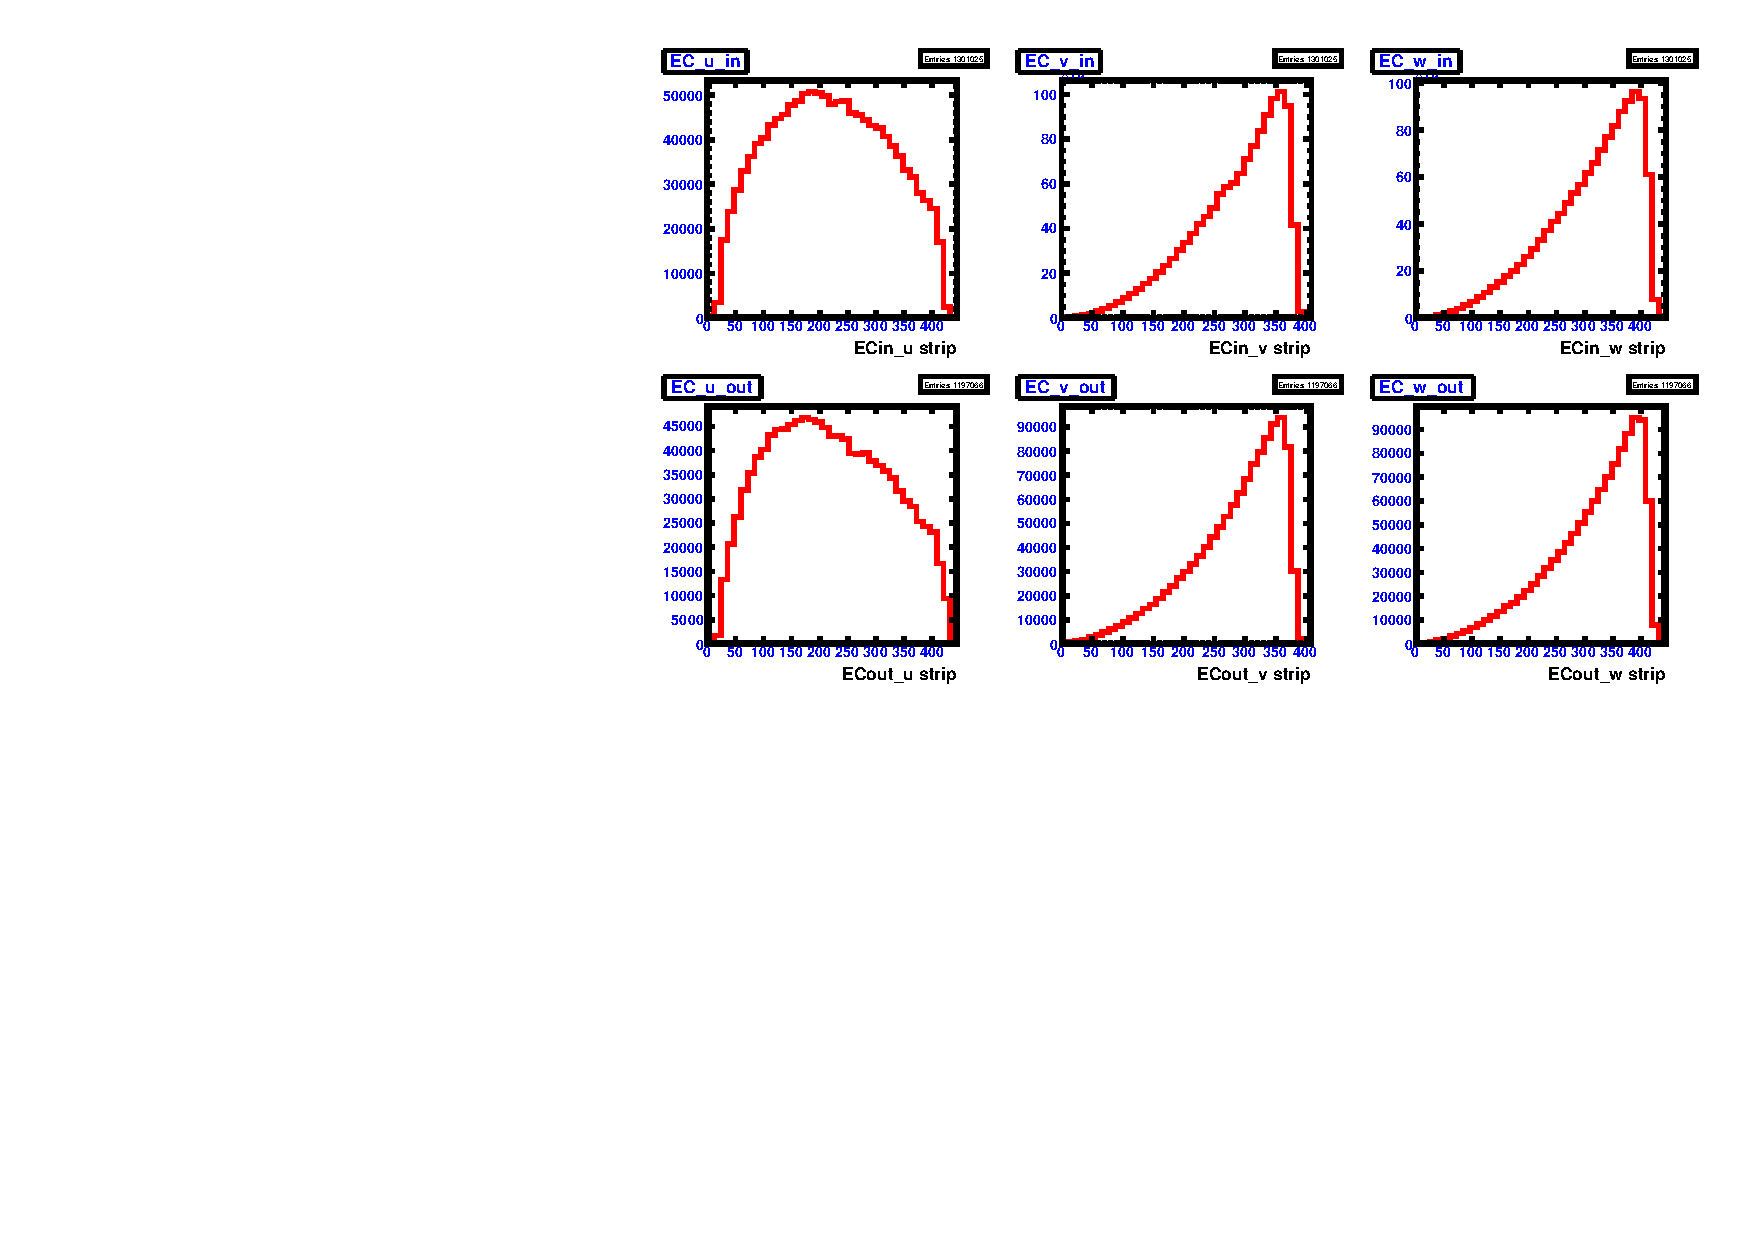
\includegraphics[width=\figwidth, height=3.5in,valign=c]{\grpath/analysis/FIDUCIAL_CUTS/EC/pim_ecuvw_NOKnockout_sec4.pdf}\label{fig:EC_II_IV}} \\

      \caption {Inefficient \abbr{EC} $u$, $v$, $w$ strips vs. $\phi$ for sector 4 in \abbr{CLAS} $e^{-} \ $ data~(\ref{fig:EC_I_IV}), notation the same as Fig.~\ref{fig:neg:ec.sec5}. Number of hits vs. inefficient \abbr{EC} $u$, $v$, $w$ strips for sector 4 for $e^-$ data~(\ref{fig:EC_II_IV}). Notation same as in Fig.~\ref{fig:neg.ecstrip.sec5}.}
        \label{fig:EC_no_IV}
\end{figure}



\begin{figure}[!ht]
  \centering
  \subfloat[][]{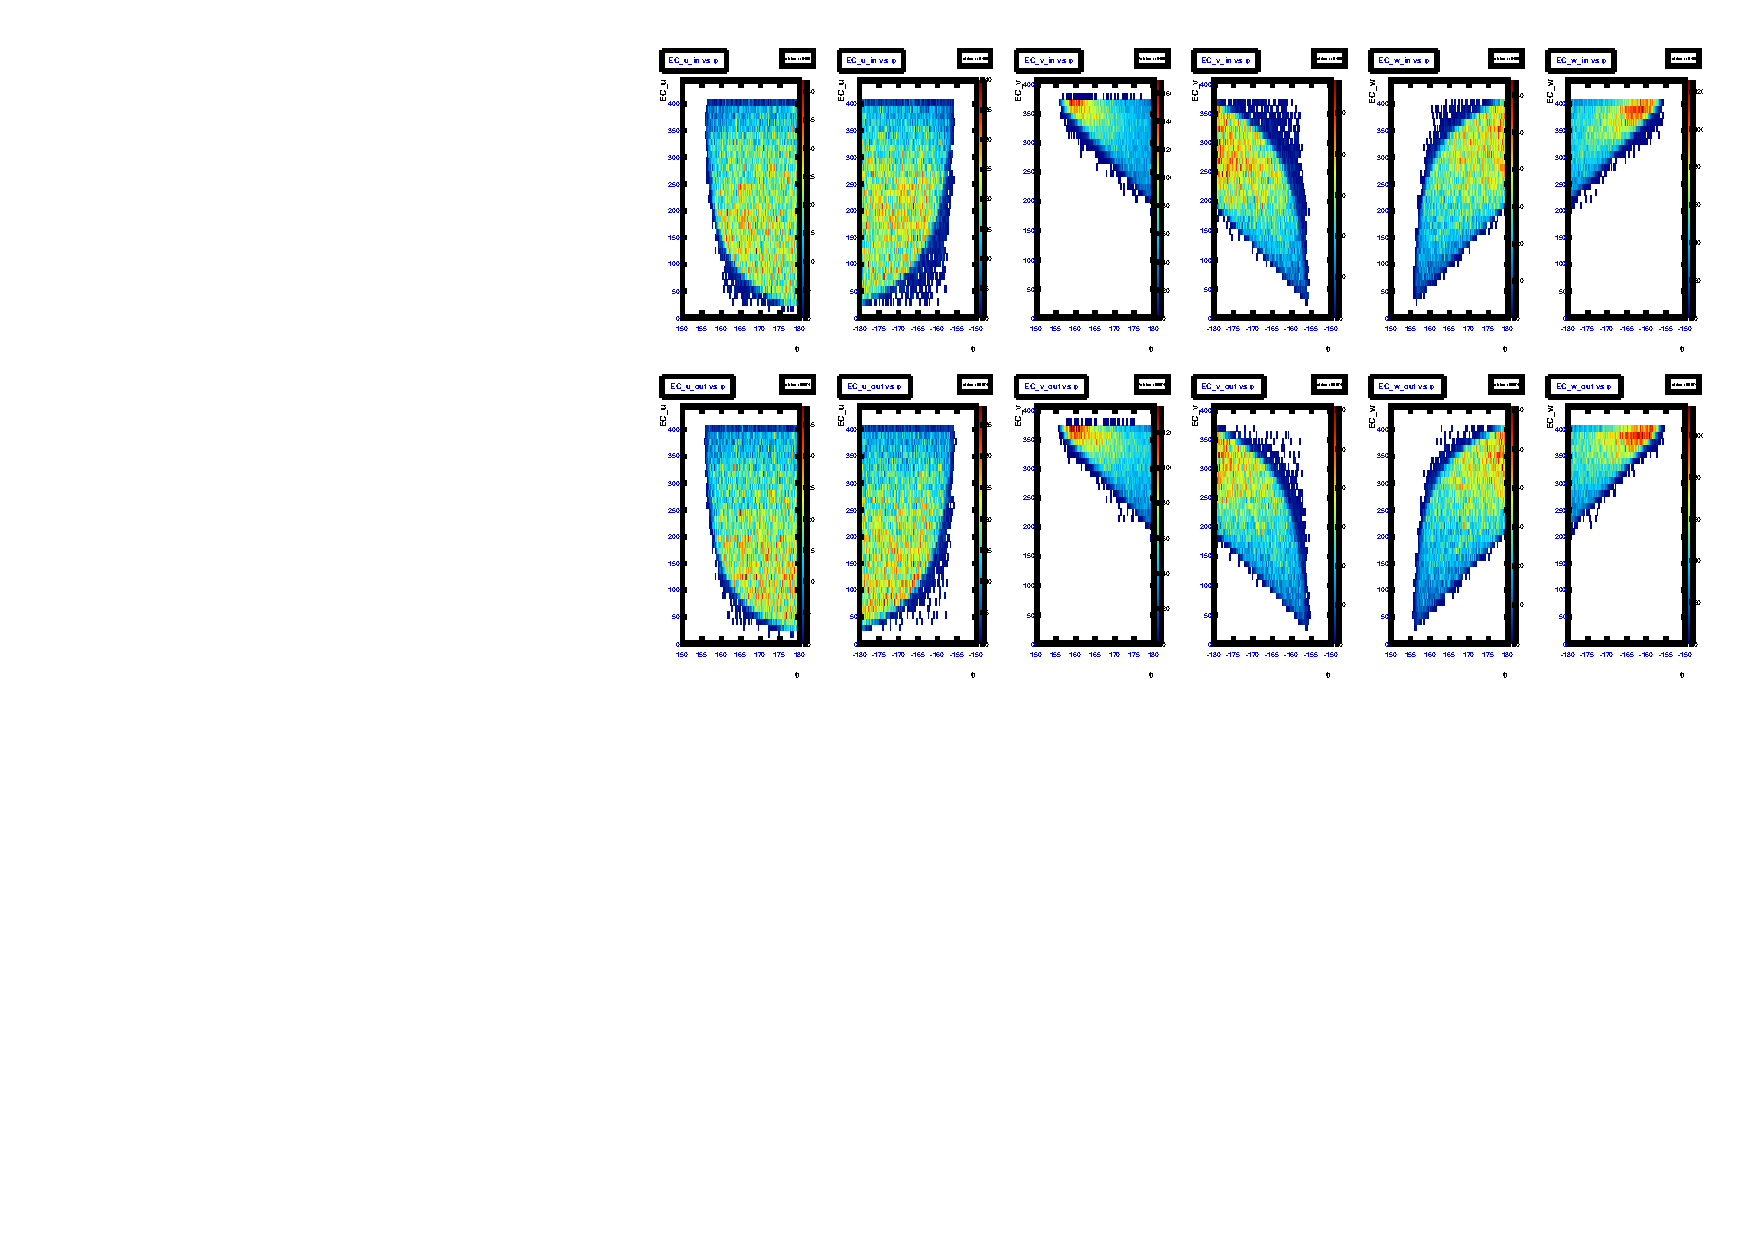
\includegraphics[width=\figwidth, height=3.5in,valign=c]{\grpath/analysis/FIDUCIAL_CUTS/EC/pim_ecuvw_phi_afterGeoFid_sec4.pdf}\label{fig:EC_III_IV}} \quad
  \\
  \subfloat[][]{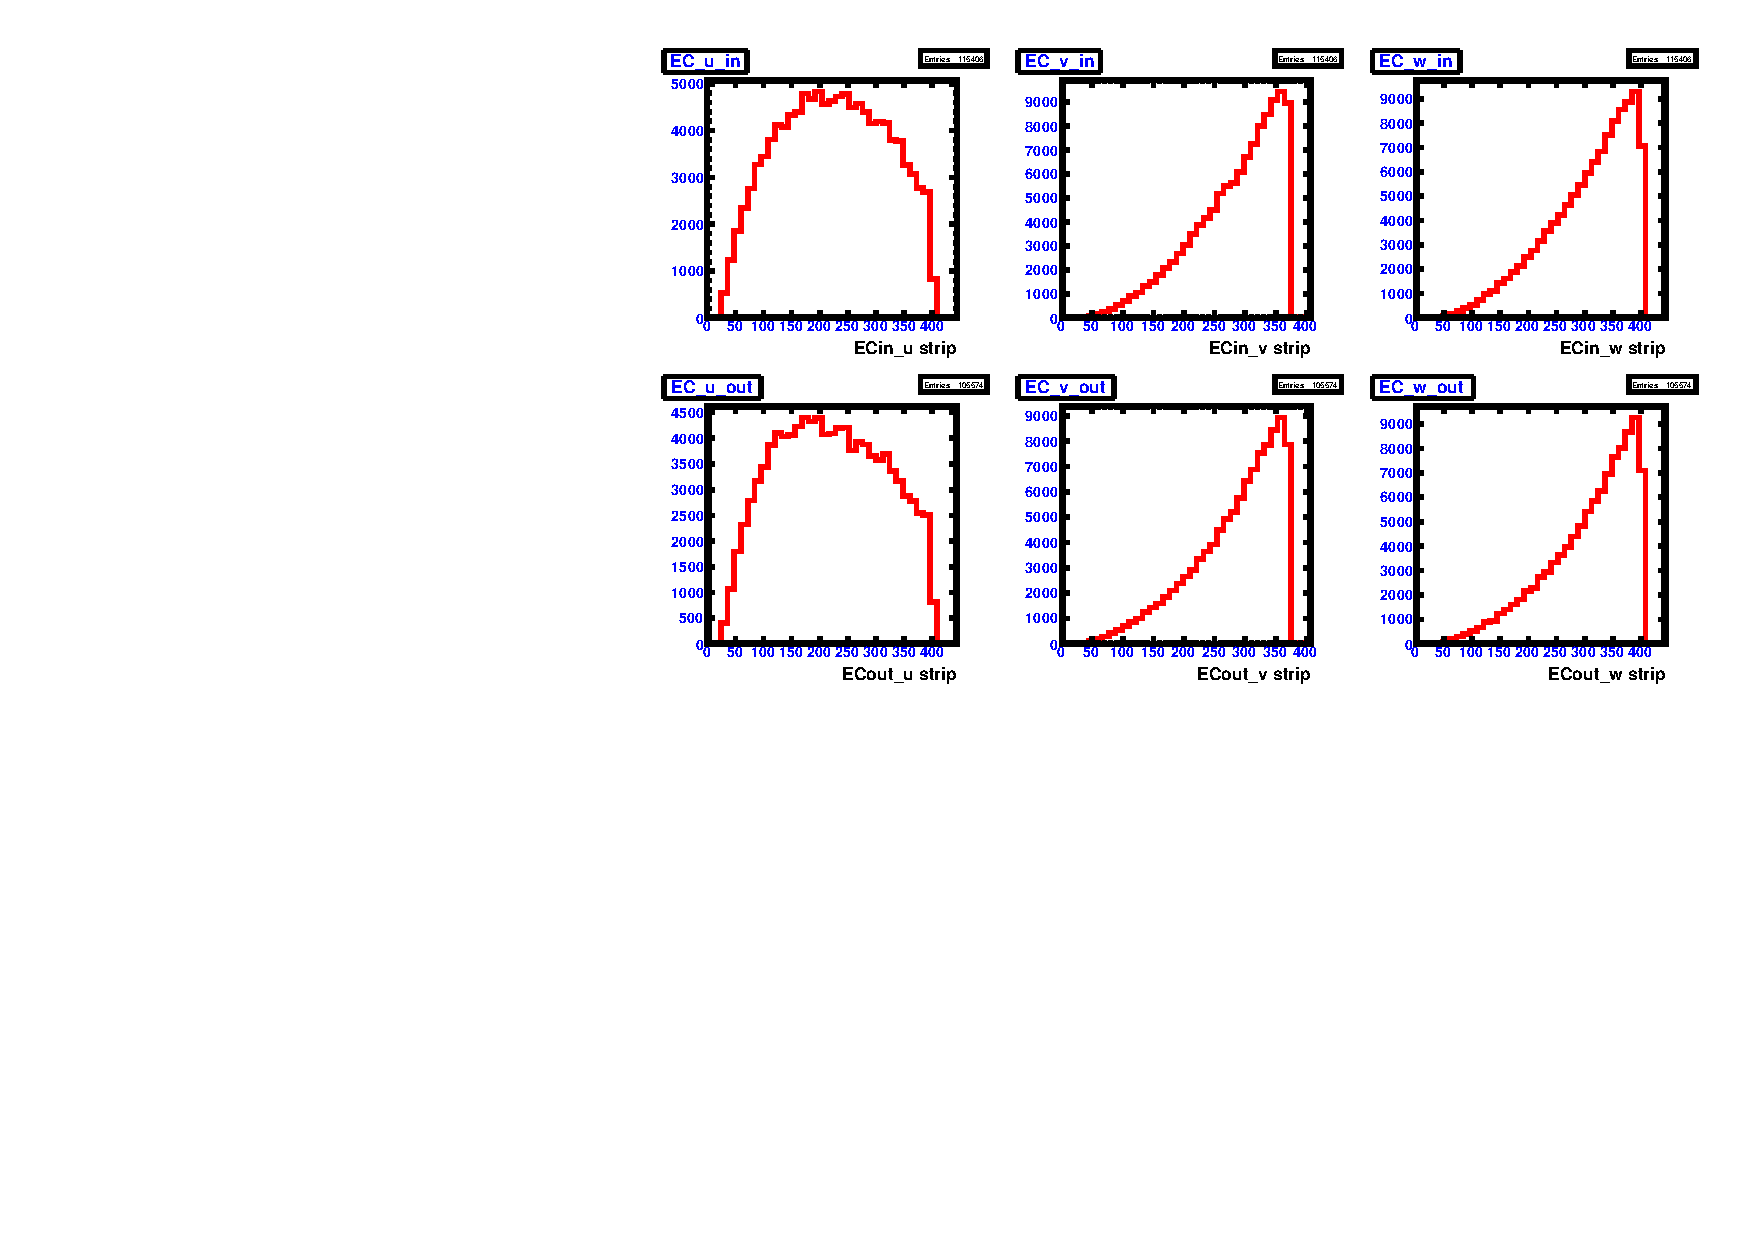
\includegraphics[width=\figwidth, height=3.5in,valign=c]{\grpath/analysis/FIDUCIAL_CUTS/EC/pim_ecuvw_afterGeoFid_sec4.pdf}\label{fig:EC_IV_IV}} \\

      \caption {\abbr{EC} $u$, $v$, $w$ strips vs. $\phi$ for sector 4 with fiducial cuts and inefficient paddle knockouts applied to $e^-$ data~(\ref{fig:EC_III_IV}), notation the same as Fig.~\ref{fig:neg:ec.sec5_cut}. Number of hits vs. \abbr{EC} $u$, $v$, $w$ strips for sector 4 with fiducial cuts and inefficient paddle knockouts applied to $e^-$ data~(\ref{fig:EC_IV_IV}). Notation same as in Fig.~\ref{fig:neg.ecstrip.sec5_cut}.}
        \label{fig:EC_cut_IV}
\end{figure}


% % % %SECTOR 5
\begin{figure}[!ht]
  \centering
  \subfloat[][]{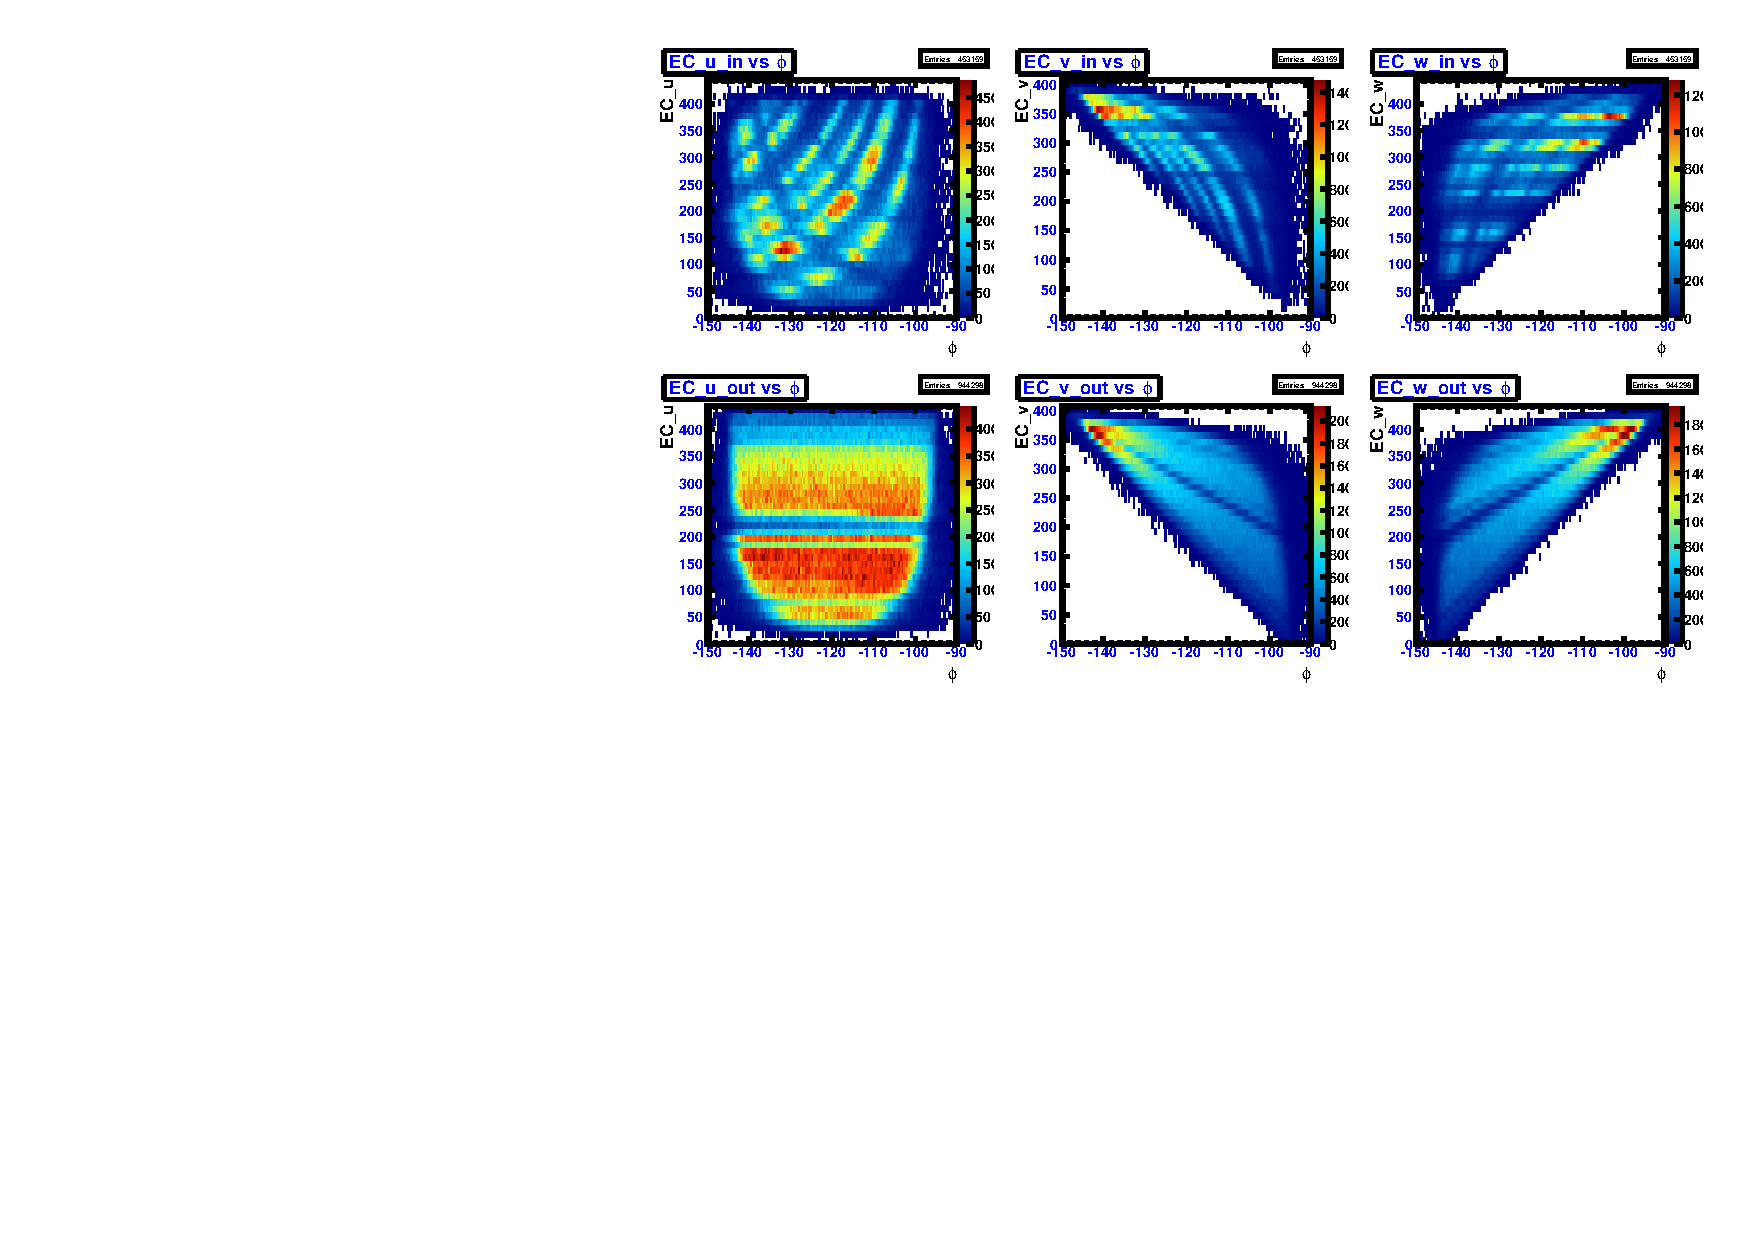
\includegraphics[width=\figwidth, height=3.5in,valign=c]{\grpath/analysis/FIDUCIAL_CUTS/EC/pim_ecuvw_phi_NOKnockout_sec5.pdf}\label{fig:EC_I_V}} \quad
  \\
  \subfloat[][]{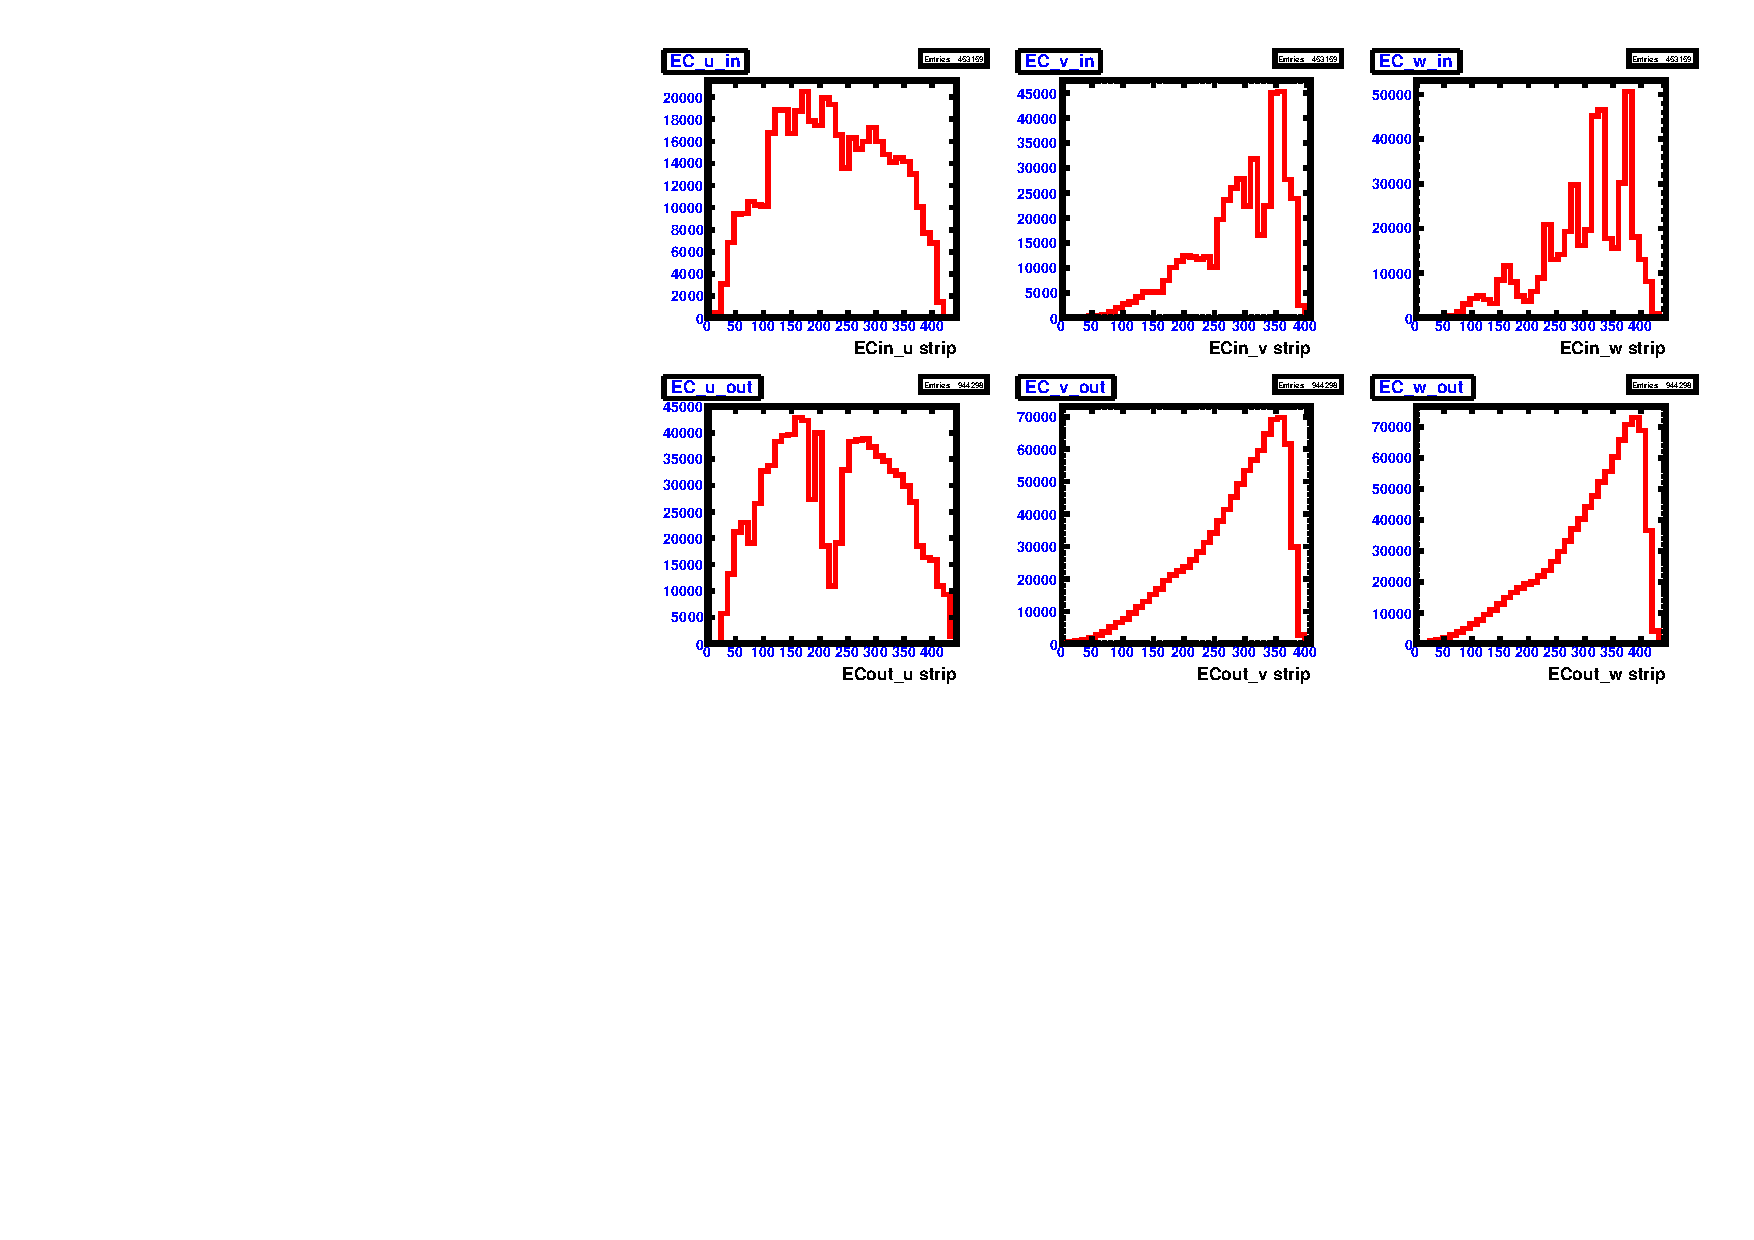
\includegraphics[width=\figwidth, height=3.5in,valign=c]{\grpath/analysis/FIDUCIAL_CUTS/EC/pim_ecuvw_NOKnockout_sec5.pdf}\label{fig:EC_II_V}} \\

      \caption {Inefficient \abbr{EC} $u$, $v$, $w$ strips vs. $\phi$ for sector 5 in \abbr{CLAS} $e^{-} \ $ data~(\ref{fig:EC_I_V}), notation the same as Fig.~\ref{fig:neg:ec.sec5}. Number of hits vs. inefficient \abbr{EC} $u$, $v$, $w$ strips for sector 5 for $e^-$ data~(\ref{fig:EC_II_V}). Notation same as in Fig.~\ref{fig:neg.ecstrip.sec5}.}
        \label{fig:EC_no_V}
\end{figure}



\begin{figure}[!ht]
  \centering
  \subfloat[][]{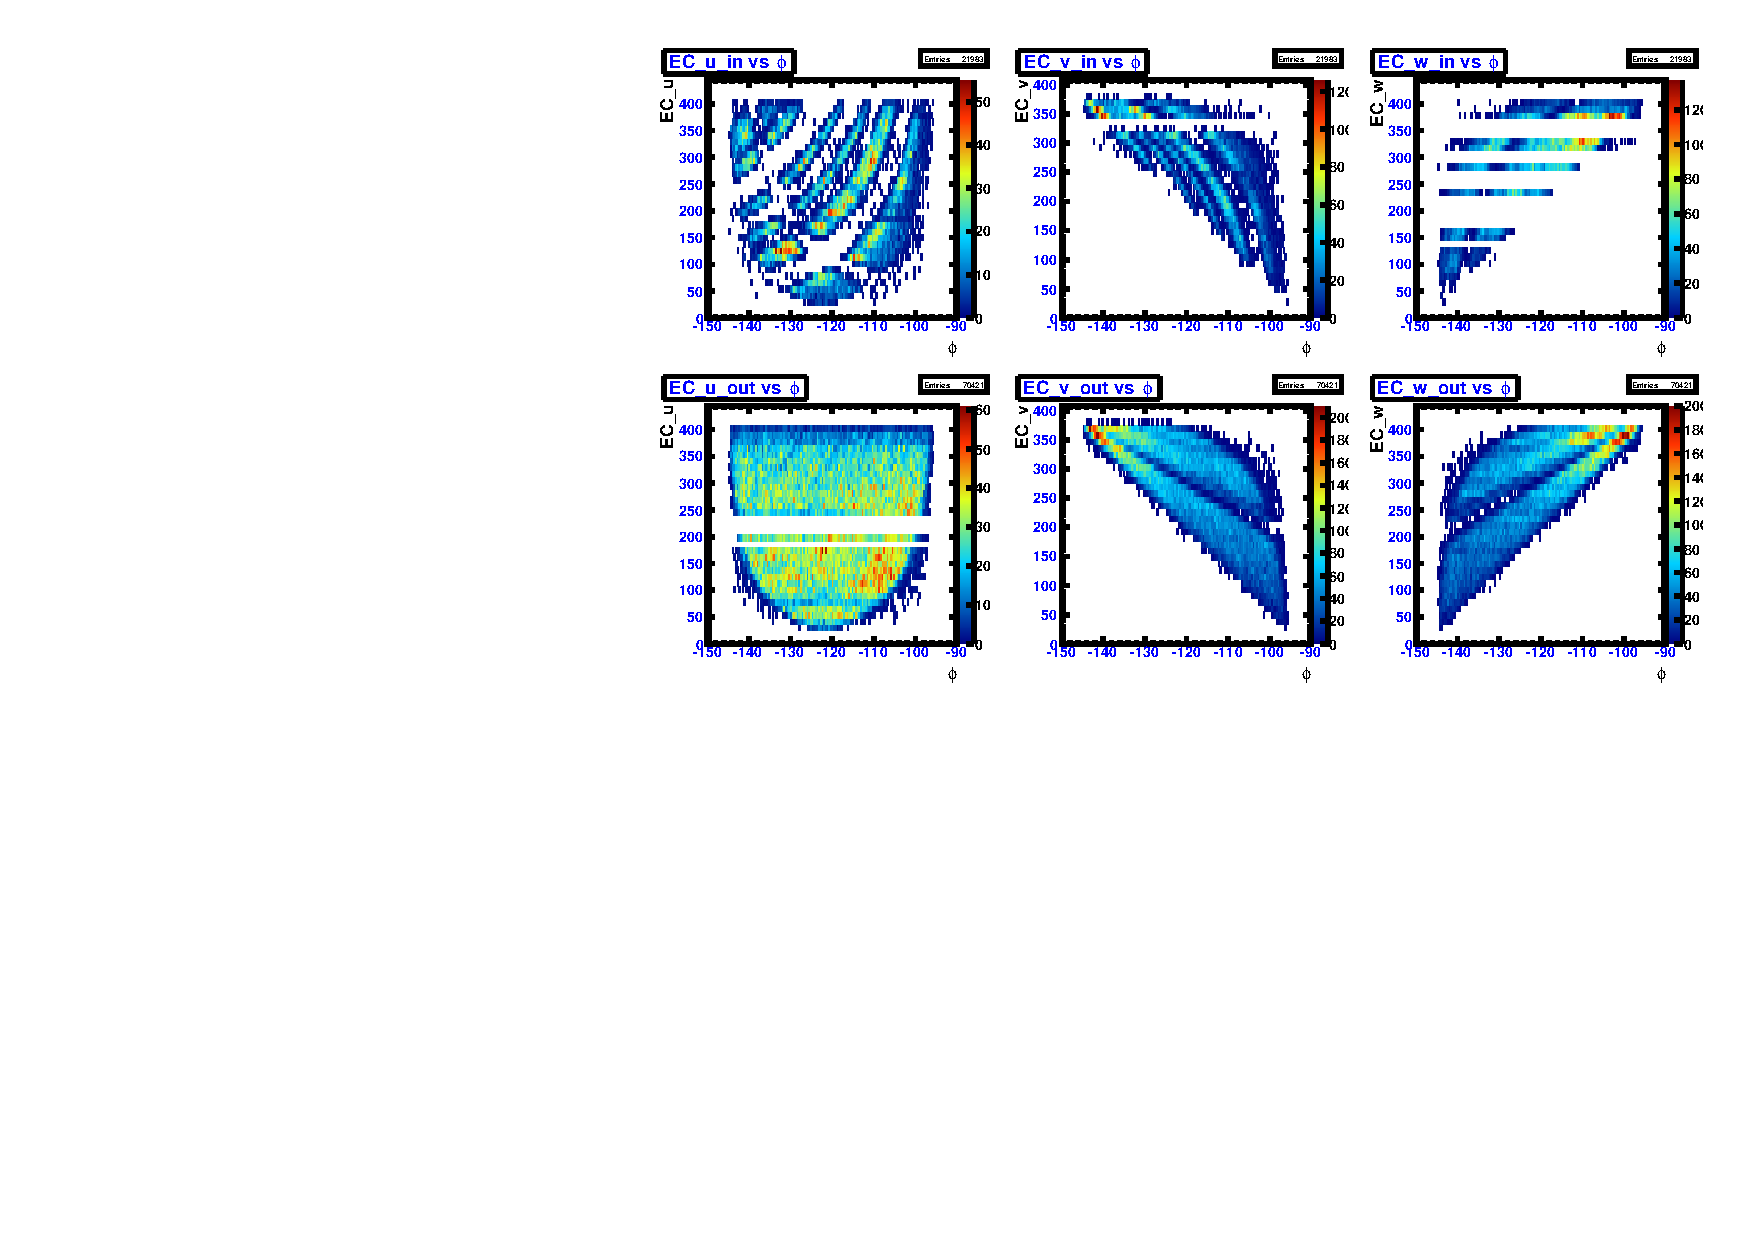
\includegraphics[width=\figwidth, height=3.5in,valign=c]{\grpath/analysis/FIDUCIAL_CUTS/EC/pim_ecuvw_phi_afterGeoFid_sec5.pdf}\label{fig:EC_III_V}} \quad
  \\
  \subfloat[][]{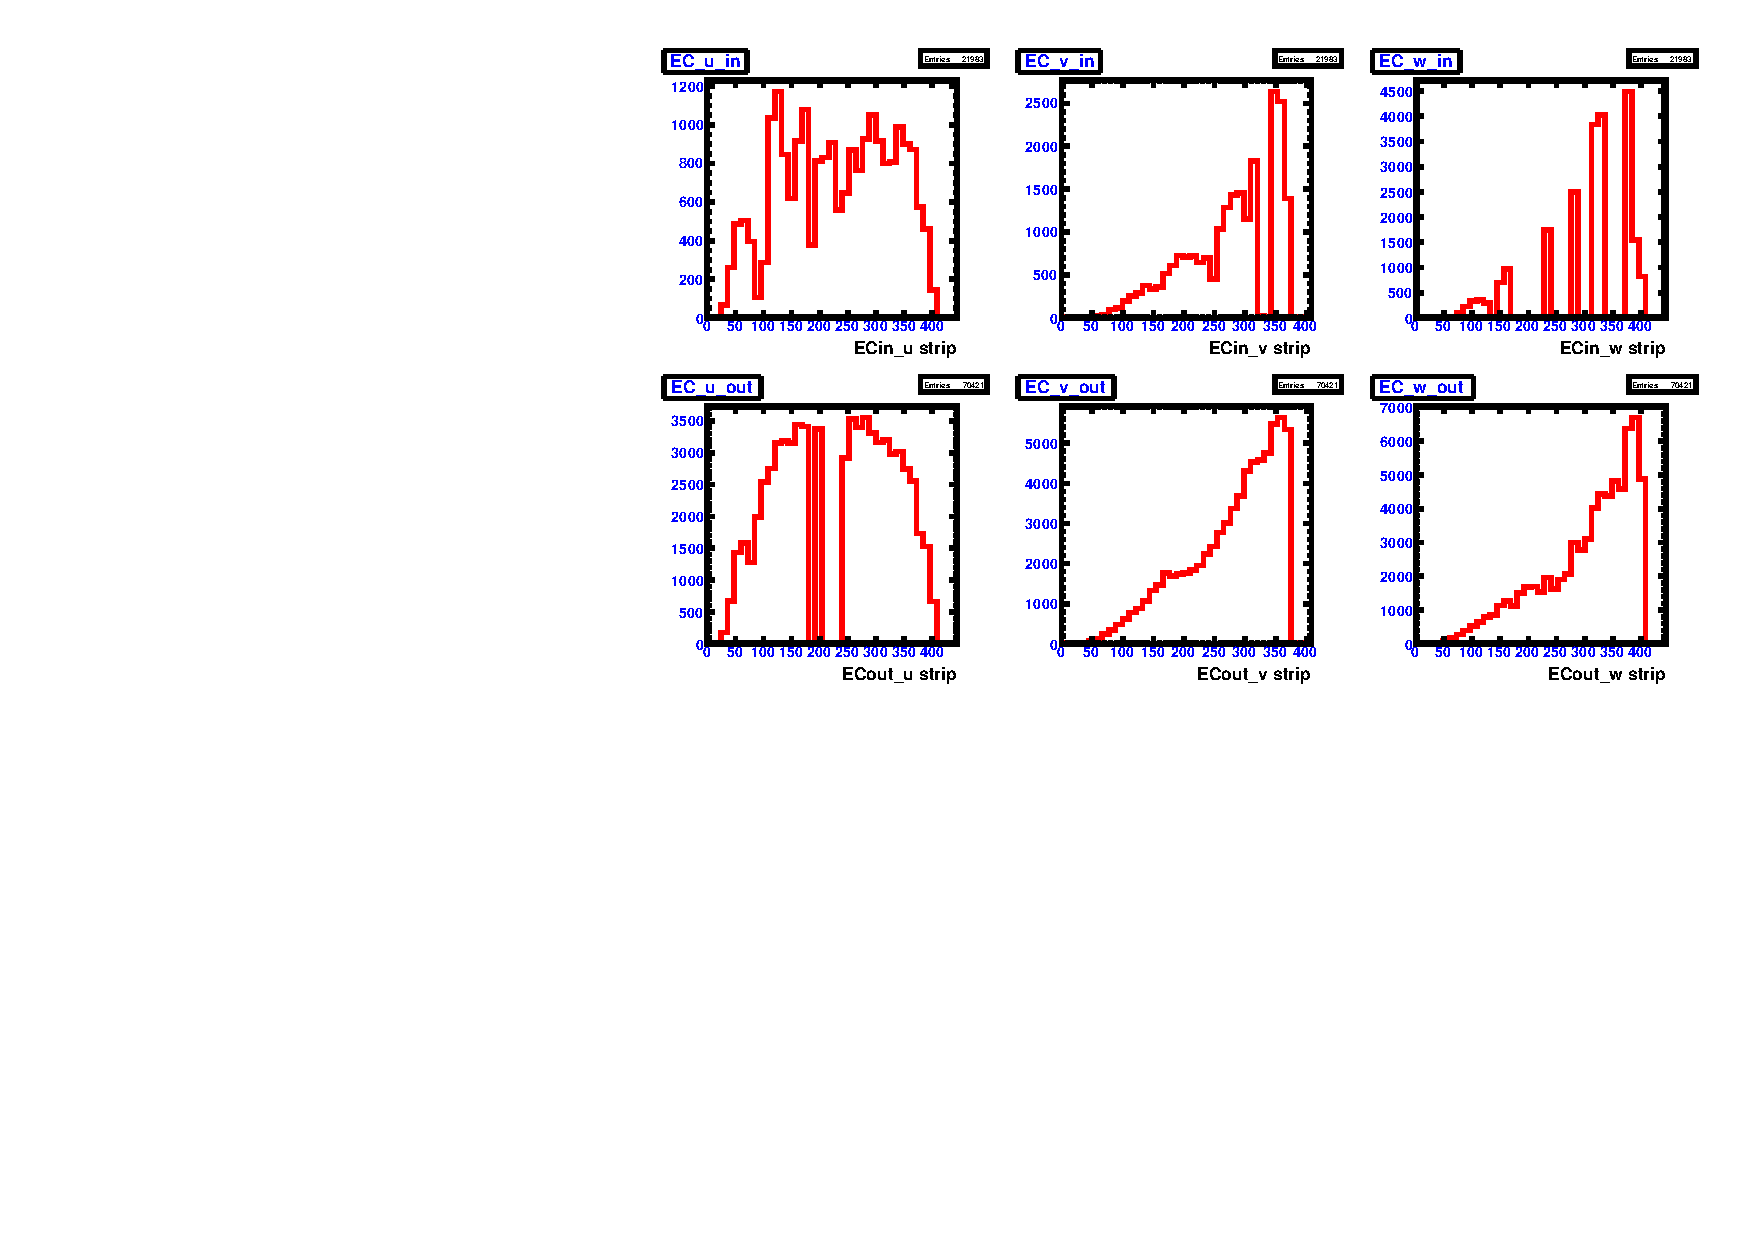
\includegraphics[width=\figwidth, height=3.5in,valign=c]{\grpath/analysis/FIDUCIAL_CUTS/EC/pim_ecuvw_afterGeoFid_sec5.pdf}\label{fig:EC_IV_V}} \\

      \caption {\abbr{EC} $u$, $v$, $w$ strips vs. $\phi$ for sector 5 with fiducial cuts and inefficient paddle knockouts applied to $e^-$ data~(\ref{fig:EC_III_V}), notation the same as Fig.~\ref{fig:neg:ec.sec5_cut}. Number of hits vs. \abbr{EC} $u$, $v$, $w$ strips for sector 5 with fiducial cuts and inefficient paddle knockouts applied to $e^-$ data~(\ref{fig:EC_IV_V}). Notation same as in Fig.~\ref{fig:neg.ecstrip.sec5_cut}.}
        \label{fig:EC_cut_V}
\end{figure}

% % % %SECTOR 6
\begin{figure}[!ht]
  \centering
  \subfloat[][]{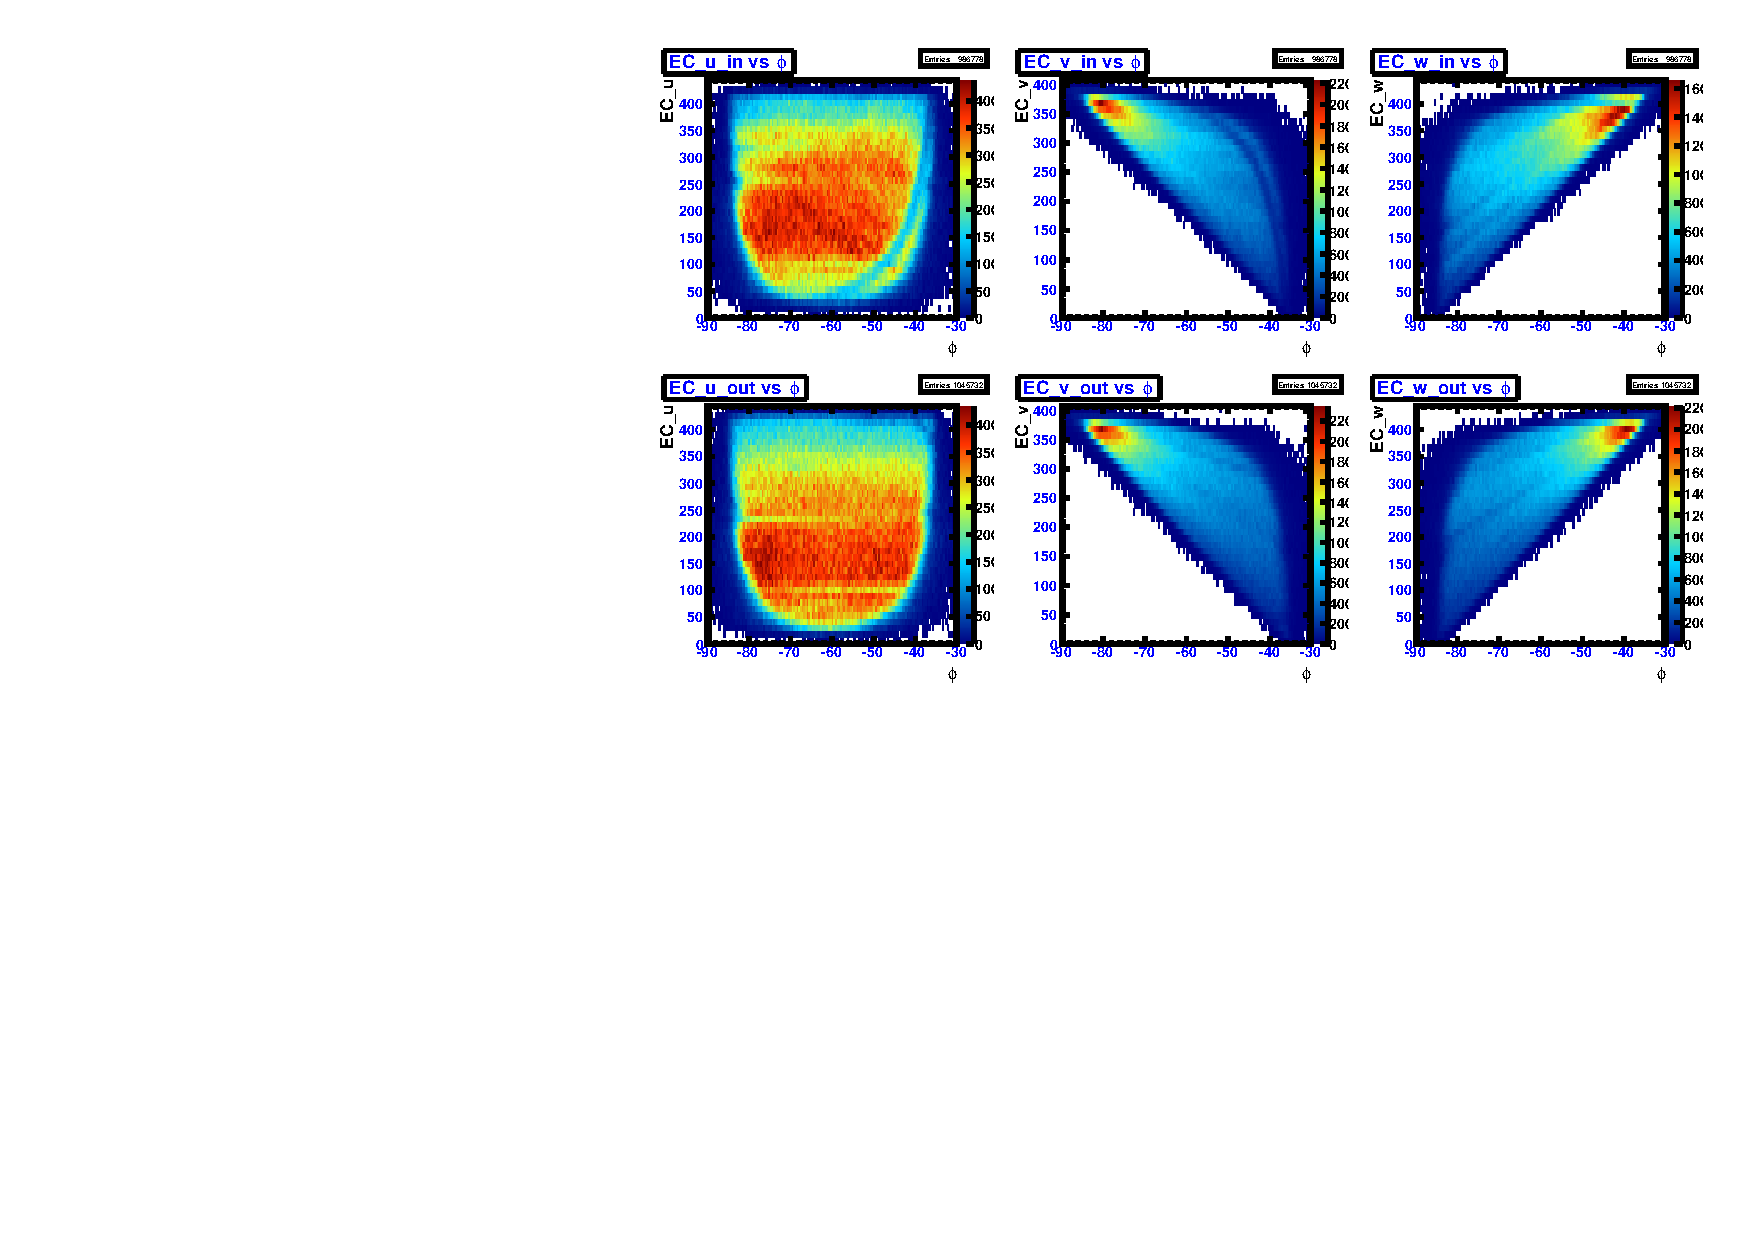
\includegraphics[width=\figwidth, height=3.5in,valign=c]{\grpath/analysis/FIDUCIAL_CUTS/EC/pim_ecuvw_phi_NOKnockout_sec6.pdf}\label{fig:EC_I_VI}} \quad
  \\
  \subfloat[][]{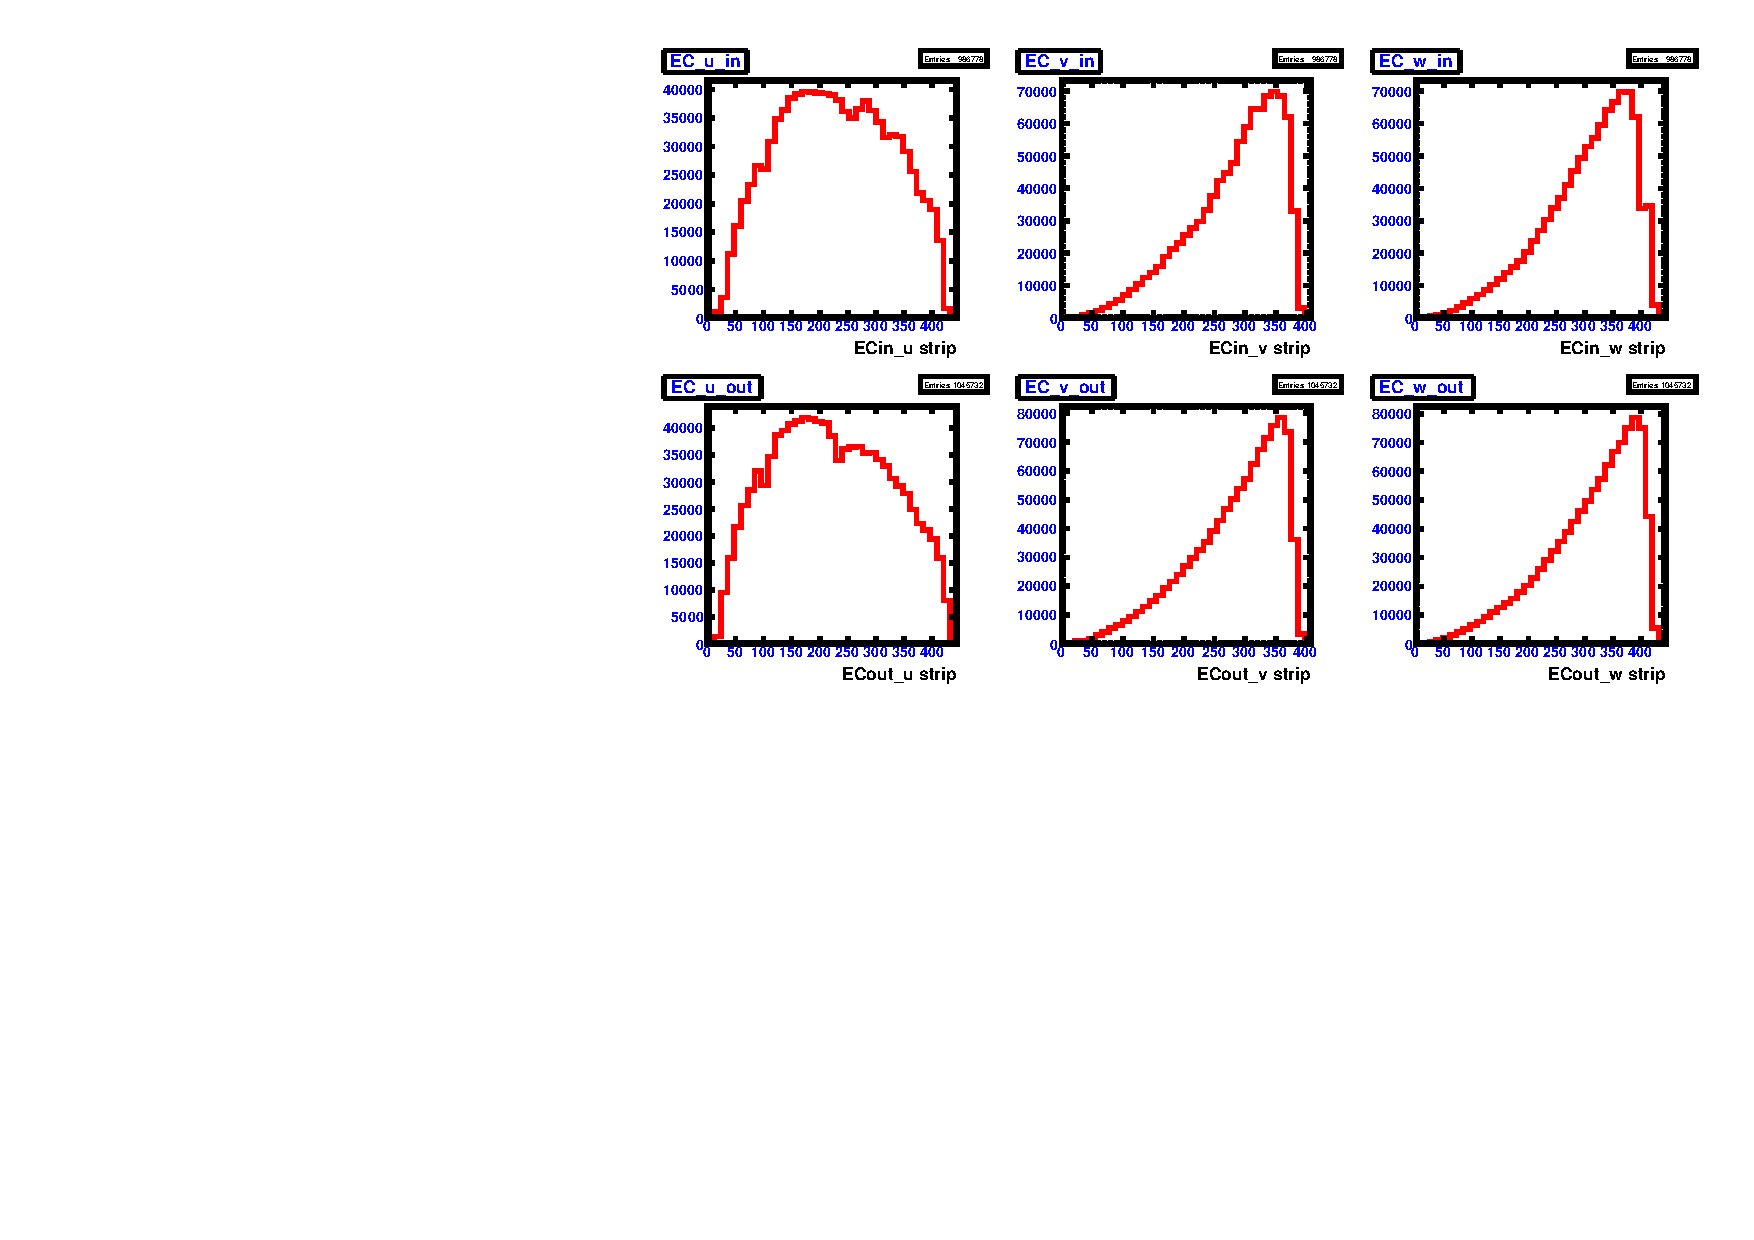
\includegraphics[width=\figwidth, height=3.5in,valign=c]{\grpath/analysis/FIDUCIAL_CUTS/EC/pim_ecuvw_NOKnockout_sec6.pdf}\label{fig:EC_II_VI}} \\

      \caption {Inefficient \abbr{EC} $u$, $v$, $w$ strips vs. $\phi$ for sector 6 in \abbr{CLAS} $e^{-} \ $ data~(\ref{fig:EC_I_VI}), notation the same as Fig.~\ref{fig:neg:ec.sec5}. Number of hits vs. inefficient \abbr{EC} $u$, $v$, $w$ strips for sector 6 for $e^-$ data~(\ref{fig:EC_II_VI}). Notation same as in Fig.~\ref{fig:neg.ecstrip.sec5}.}
        \label{fig:EC_no_VI}
\end{figure}



\begin{figure}[!ht]
  \centering
  \subfloat[][]{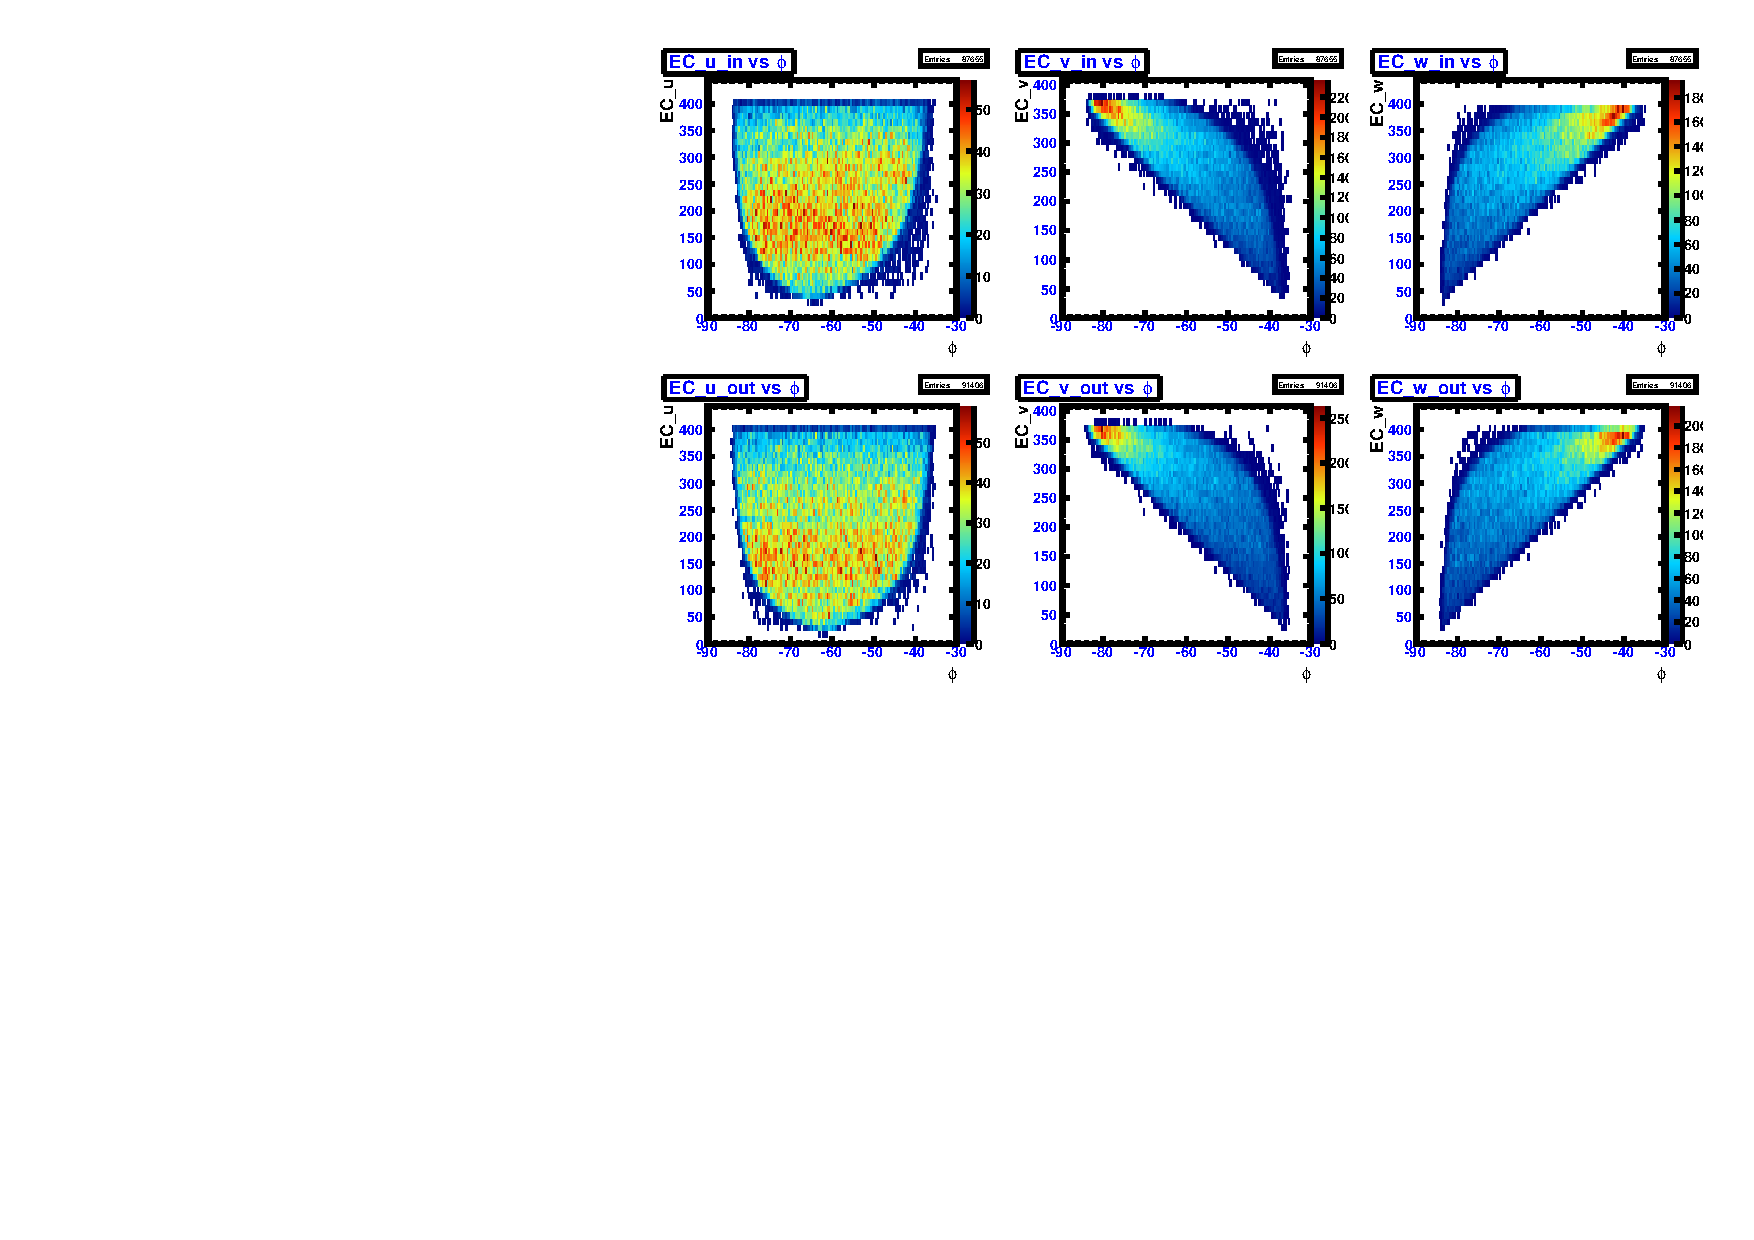
\includegraphics[width=\figwidth, height=3.5in,valign=c]{\grpath/analysis/FIDUCIAL_CUTS/EC/pim_ecuvw_phi_afterGeoFid_sec6.pdf}\label{fig:EC_III_VI}} \quad
  \\
  \subfloat[][]{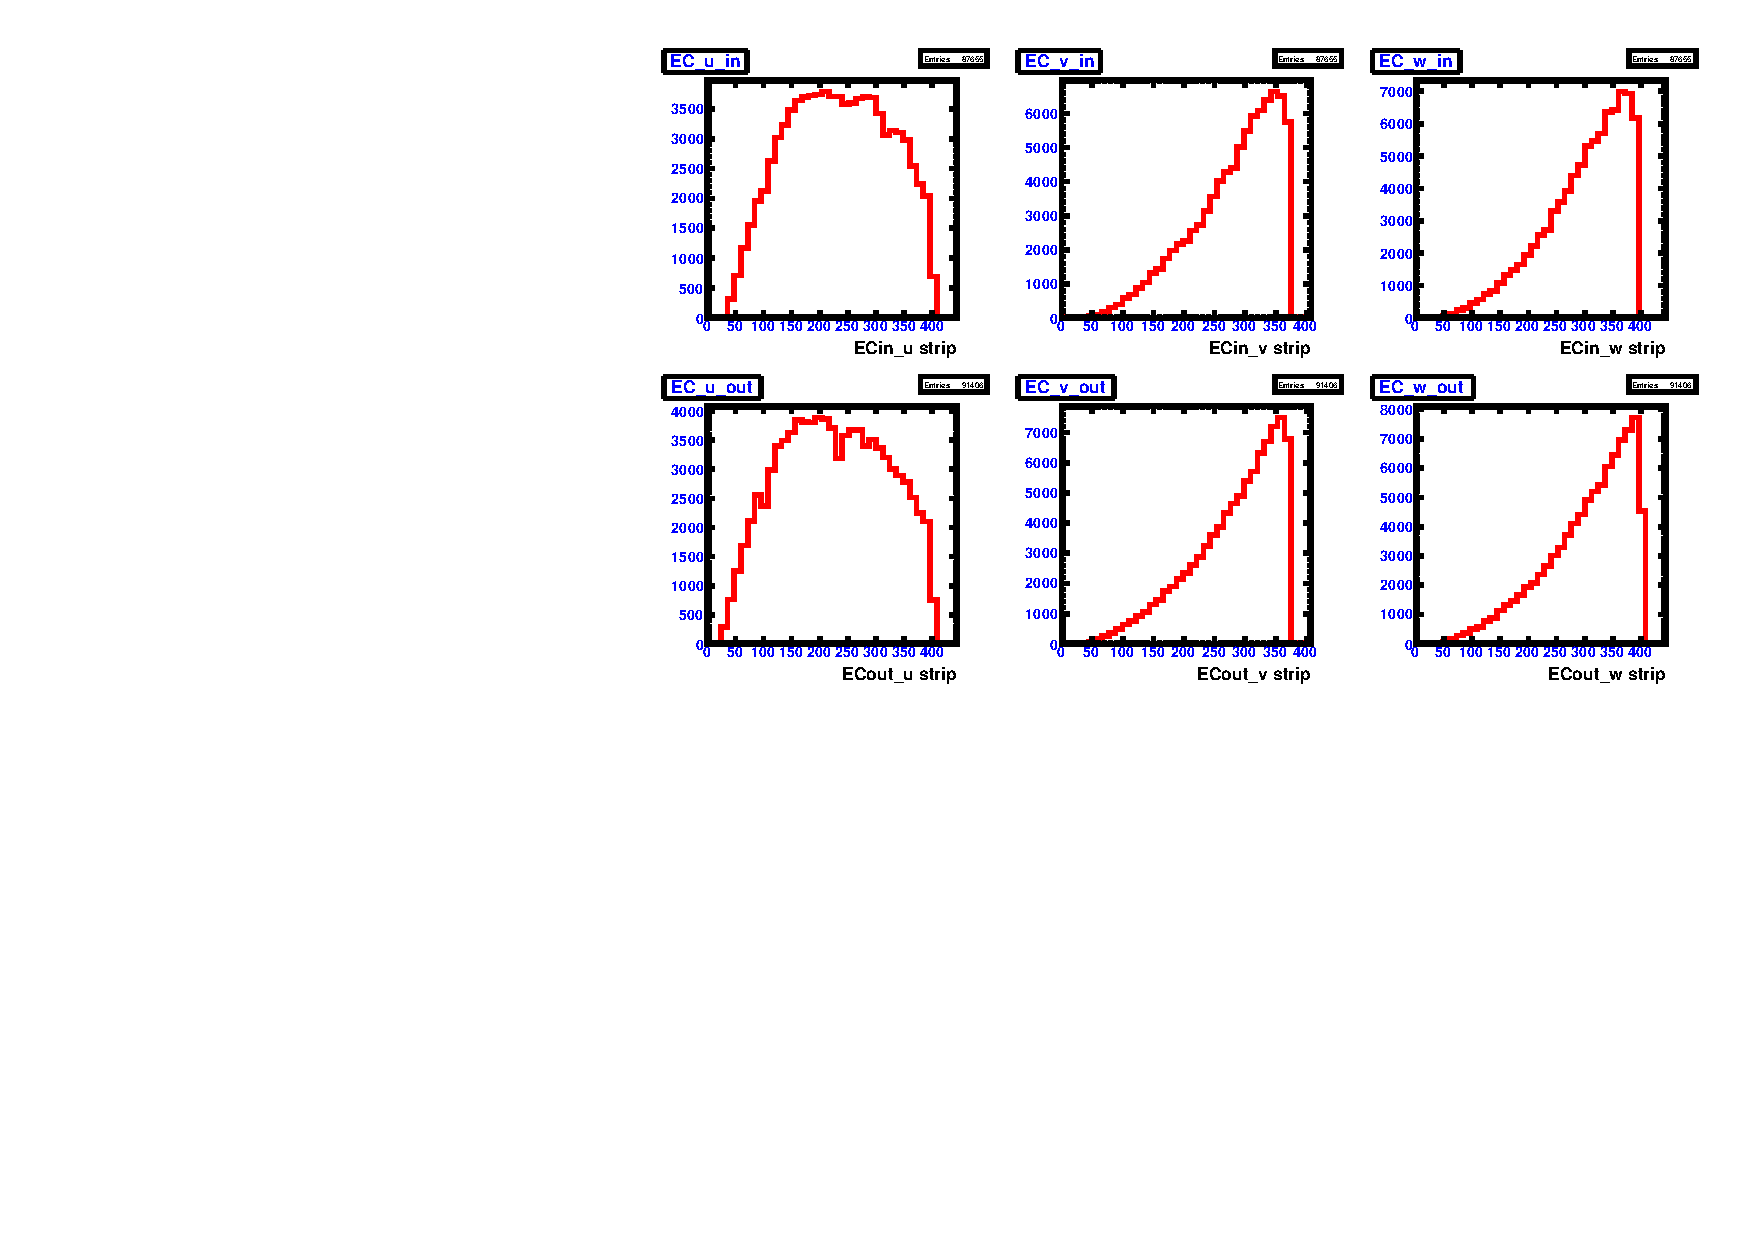
\includegraphics[width=\figwidth, height=3.5in,valign=c]{\grpath/analysis/FIDUCIAL_CUTS/EC/pim_ecuvw_afterGeoFid_sec6.pdf}\label{fig:EC_IV_VI}} \\

      \caption {\abbr{EC} $u$, $v$, $w$ strips vs. $\phi$ for sector 6 with fiducial cuts and inefficient paddle knockouts applied to $e^-$ data~(\ref{fig:EC_III_VI}), notation the same as Fig.~\ref{fig:neg:ec.sec5_cut}. Number of hits vs. \abbr{EC} $u$, $v$, $w$ strips for sector 6 with fiducial cuts and inefficient paddle knockouts applied to $e^-$ data~(\ref{fig:EC_IV_VI}). Notation same as in Fig.~\ref{fig:neg.ecstrip.sec5_cut}.}
        \label{fig:EC_cut_VI}
\end{figure}

\FloatBarrier

